\documentclass[12pt]{report}
\usepackage[fontsize=13pt]{scrextend}
\usepackage[a4paper,top=2cm,bottom=2cm,left=3cm,right=2cm]{geometry}
% \usepackage{svg}
\usepackage{tgtermes}
\usepackage{fontspec}
\usepackage[numbers]{natbib}
% \usepackage{pgfsys}
% \usepackage{transparent}
\usepackage{indentfirst}
\usepackage{eso-pic}
\usepackage{tikz}
\usepackage{fancyhdr}
\usepackage{lastpage}
\usepackage{tabularx}
\usepackage{amsmath}
\usetikzlibrary{positioning,arrows.meta,backgrounds,fit,calc}
\usepackage{anyfontsize}
\usepackage{float}
\usepackage{titlesec}
\usepackage{listings}
\usepackage{lscape}
\linespread{1.5}
\usepackage{hyperref}
\usepackage{longtable}
\usepackage[utf8]{inputenc}
\usepackage{glossaries}
\usepackage{makecell}
\usepackage{longtable}
\usepackage{multirow}
\usepackage{array}
\usepackage{pdflscape}
\hypersetup{
    colorlinks=true,
    citecolor=blue,
    filecolor=black,
    linkcolor=black,
    urlcolor=blue
}
\usepackage{subcaption}
\usepackage{enumitem}
\usepackage{xcolor}
\emergencystretch=3em
\hyphenpenalty=500
\tolerance=1000

\definecolor{myjsoncolor}{RGB}{128, 0, 128} % You can customize this color

\lstdefinelanguage{json}{
    basicstyle=\ttfamily\small\color{myjsoncolor},
    numbers=left,
    numberstyle=\tiny\color{gray},
    stepnumber=1,
    numbersep=5pt,
    showstringspaces=false,
    breaklines=true,
    frame=single,
    backgroundcolor=\color{white},
    literate=
     *{:}{{{\color{black}:}}}{1}
      {,}{{{\color{black},}}}{1}
}

\lstset{
    basicstyle=\small\ttfamily, % Small font size
    numbers=left,
    frame=single,
}
\usepackage{pgfplots} % Required for the TikZ figure
\pgfplotsset{compat=1.17} % Ensure compatibility with the latest version of pgfplots


% Define chapter font size to be 15pt
\titleformat{\chapter}[display]{\normalfont\huge\bfseries}{\chaptertitlename\ \thechapter}{20pt}{\Huge}

\makeglossaries

\newglossaryentry{AI}
{
    name=AI,
    description={Artificial Intelligence}
}

\newglossaryentry{API}
{
    name=API,
    description={Application Programming Interface}
}

\newglossaryentry{CSV}
{
    name=CSV,
    description={Comma Separated Values}
}

\newglossaryentry{ELT}
{
    name=ELT,
    description={Extract - Load - Transform}
}

\newglossaryentry{ETL}
{
    name=ETL,
    description={Extract - Transform - Load}
}

\newglossaryentry{GCP}
{
    name=GCP,
    description={Google Cloud Platform}
}

\newglossaryentry{HDFS}
{
    name=HDFS,
    description={Hadoop Distributed File System}
}

\newglossaryentry{HPC}
{
    name=HPC,
    description={High-Performance Computing}
}

\newglossaryentry{IAM}
{
    name=IAM,
    description={Identity Access Management}
}

\newglossaryentry{IoT}
{
    name=IoT,
    description={Internet of Things}
}

\newglossaryentry{IT}
{
    name=IT,
    description={Information Technology}
}

\newglossaryentry{PDF}
{
    name=PDF,
    description={Portable Document Format}
}

\newglossaryentry{SAS}
{
    name=SAS,
    description={Shared Access Signature}
}

\newglossaryentry{SMT}
{
    name=SMT,
    description={Single Message Transform}
}

\newglossaryentry{UI}
{
    name=UI,
    description={User Interface}
}

\newglossaryentry{YARN}
{
    name=YARN,
    description={Yet Another Resource Negotiator}
}

\setcounter{secnumdepth}{3}
\setcounter{tocdepth}{2}
\begin{document}

\input{sections/cover-page}


\setmainfont{TIMES}[
    Path = fonts/,
    Extension = .TTF,
    UprightFont = *,
    BoldFont = *BD,
    ItalicFont = *I,
    BoldItalicFont = *BI
]

\pagenumbering{roman} 
\chapter*{Instructor's Signature}

\vspace{1cm}

\makebox[0.7\linewidth][l]{\hrulefill} Date: \makebox[0.2\linewidth][l]{\hrulefill}

    \begin{flushleft}
    [Supervisor Name] (Instructor)\\
    \vspace{4cm}
    Faculty of Computer Science and Engineering
    \end{flushleft}


\chapter*{Declaration of Authenticity}

We declare that we solely conducted this project, under the supervision of [Supervisor Name] at the Faculty of Computer Science and Engineering, Vietnam National University - Ho Chi Minh City University of Technology.

We have taken care to properly acknowledge and document all external sources and references used in the project.

If there is any instance of plagiarism, we are ready to accept the consequences. Ho Chi Minh City University of Technology - Vietnam National University HCMC will not be held responsible for any copyright violations that may have occurred during my research.

\vspace{2cm}

\begin{flushright}
\begin{tabular}{r}
    Ho Chi Minh City, 2025 \\
    \textit{\textbf{Authors}} \\
    [Student 1 Name] \\
    [Student 2 Name]
\end{tabular}
\end{flushright}


\chapter*{Member Contributions}
\addcontentsline{toc}{chapter}{Member Contributions}

\noindent
\begin{tabular}{@{}p{5cm} p{8.5cm}@{}}
\textbf{Student name} & \textbf{Student ID} \\
\hline
Dang Minh Khang  & 2252287 \\
Pham Tran Dang Khoa & 2252360 \\
\hline
\end{tabular}

\vspace{1.5em}

\noindent\textbf{General / Shared Contributions}

\begin{itemize}
    \item Co-designed the high-level architecture of the dual-mode multimodal book recommendation system, integrating the behavioral graph pipeline (Pipeline~A), sequential intent pipeline (Pipeline~B), text-based HNSW search, and visual CLIP search into a unified serving stack.
    \item Jointly defined the experimental evaluation protocol, including benchmark dataset selection (Amazon Book Reviews, 3M items), metric specifications (HR@10, NDCG@10), and multilingual retrieval quality criteria across 19 languages.
    \item Conducted joint end-to-end system performance benchmarking, measuring throughput, latency, and retrieval quality across all system components under realistic load conditions.
    \item Collaborated on the authorship of the technical report, collectively covering system analysis, proposed solutions, experimental evaluation, and the application chapter.
\end{itemize}

\vspace{1em}

\noindent\textbf{Dang Minh Khang (2252287)}

\begin{itemize}
    \item Architected and implemented DIF-SASRec with decoupled content and category attention streams and a sigmoid-gated scalar fusion mechanism; conducted large-scale pretraining on 100{,}000 users to produce the shared model checkpoint used at inference time.

    \item Engineered Pipeline~A (behavioral recommendation): Cleora co-purchase graph training and behavioral embedding generation across a 375{,}000-item candidate pool, producing the graph embeddings used for candidate pre-filtering.

    \item Engineered Pipeline~B (sequential intent recommendation): DIF-SASRec online inference with per-user fine-tuning at serving time and content-veto filtering (cosine similarity threshold $\tau = 0.3$) to suppress semantically unrelated candidates.

    \item Implemented the AgentPool concurrency layer comprising 8 process-isolated inference agents, \texttt{asyncio.Queue}-based task dispatch, and pretrained CPU snapshot preloading, enabling parallel per-user fine-tuning without model reload overhead.

    \item Implemented the NLLB-200 translation quality gate with multi-hypothesis beam retry, ensuring robust query normalization and graceful fallback for noisy multilingual inputs before embedding.

    \item Formulated and implemented the active search routing logic: query-length-based short/long path differentiation, Reciprocal Rank Fusion (RRF) bypass for single-modality queries, and multi-attribute metadata filtering for author, genre, and title constraints.

    \item Designed and executed quantitative evaluations covering recommendation quality metrics (HR@10 $= 0.7886$, NDCG@10), multilingual retrieval benchmarks across 19 languages, and HNSW recall analysis against the flat exact-search baseline.

    \item Designed and conducted ablation studies systematically isolating Pipeline~A, Pipeline~B, and their combined configuration to quantify the marginal contribution of each recommendation component.
\end{itemize}

\vspace{0.5em}

\noindent\textbf{Pham Tran Dang Khoa (2252360)}

\begin{itemize}
    \item Architected the FastAPI backend service structure with \texttt{app/config.py} as the single source of configuration truth; orchestrated a full encoder-abstraction refactor across 10+ service modules to decouple model-specific logic from business logic.

    \item Designed and deployed the full infrastructure layer: Docker Compose stack (MongoDB + Redis), Redis async interaction write-queue (\texttt{RPUSH}/\texttt{BLPOP}) for non-blocking interaction ingestion, and a MongoDB dual-collection schema (\textit{interactions} + \textit{profiles}) for durable logging and user state persistence.

    \item Engineered the stateless user profile system with an async \texttt{UserProfileManager} backed by \texttt{motor}, per-user async locking to prevent concurrent write conflicts, and a lazy JSON-to-MongoDB migration engine for zero-downtime backward-compatible data migration.

    \item Proposed and implemented FAISS HNSW indexing and Tantivy BM25 as a high-performance replacement for Python \texttt{rank-bm25}, achieving a 340$\times$ retrieval speedup while preserving ranking quality through Reciprocal Rank Fusion with the dense HNSW results.

    \item Implemented the Cleora incremental refit infrastructure: \texttt{asyncio.Event}-gated refit scheduling to prevent concurrent rebuilds, \texttt{reload\_cleora()} atomic hot-swap for zero-downtime graph index updates, and \texttt{CLEORA\_REFIT\_THRESHOLD} environment-variable configuration for operator control over refit frequency.

    \item Designed and implemented the full multilingual translation pipeline: Lingua language identification, NLLB-200 neural translation across 19 languages, \texttt{@lru\_cache(maxsize=2048)} translation memoization to eliminate redundant inference, and deterministic startup warmup to eliminate cold-start latency on the first request.

    \item Applied a comprehensive suite of backend performance optimizations: FP16 model weight casting, BGE-M3 sequence-length capping (\texttt{max\_seq\_length=64}), LRU text-embedding cache (\texttt{maxsize=4096}), \texttt{anyio} task-group parallel encoding for concurrent multi-field queries, Pydantic bypass via \texttt{JSONResponse} for reduced serialization overhead, and response payload pruning to minimize network transfer.

    \item Designed and implemented the React frontend application, providing the primary user-facing interface for search, recommendation browsing, and interaction logging.
\end{itemize}

\vspace{1.5cm}
\begin{flushright}
\begin{tabular}{r}
    Ho Chi Minh City, 2026 \\
    \textit{\textbf{Authors}} \\
    Dang Minh Khang \\
    Pham Tran Dang Khoa \\
\end{tabular}
\end{flushright}


\chapter*{Acknowledgement}

The authors would like to express sincere gratitude to [Supervisor Name], lecturer at the Faculty of Computer Science and Engineering, Ho Chi Minh City University of Technology, for the continuous guidance, constructive feedback, and encouragement provided throughout the duration of this capstone project.
Their expertise and patience have been invaluable in shaping both the technical direction and academic presentation of this work.

Gratitude is also extended to the Faculty of Computer Science and Engineering for providing access to computational resources and a stimulating research environment.
The knowledge and skills developed through the curriculum formed the essential foundation upon which this project was built.

The authors further acknowledge the open-source communities behind the tools and datasets used in this work, including the Amazon Book Reviews dataset, the BGE-M3 encoder, the FAISS library, and the DIF-SASRec architecture — without which the experiments reported here would not have been feasible.

Finally, the authors wish to thank their families and friends for their unwavering support and encouragement throughout this journey.

\vspace{2cm}

\begin{flushright}
\begin{tabular}{r}
    Ho Chi Minh City, 2025 \\
    \textit{\textbf{Authors}} \\
    [Student 1 Name] \\
    [Student 2 Name]
\end{tabular}
\end{flushright}



\chapter*{Abstract}

This report presents the design, implementation, and evaluation of a dual-mode multimodal book recommendation system built on a data platform with modular ingestion, storage, and retrieval components, backed by MongoDB for persistent interaction logs and Redis as an asynchronous interaction write-queue.
The system addresses two distinct recommendation scenarios: proactive candidate generation based on long-term behavioural history, and intent-sensitive ranking based on recent interaction sequences.

Two complementary pipelines are proposed.
Pipeline~A retrieves candidates through a Cleora co-purchase graph embedding index covering 375{,}280 items, then re-ranks them using a BGE-M3 semantic profile vector constructed by mean-pooling the user's interaction embeddings.
Pipeline~B applies a DIF-SASRec transformer with decoupled content and category attention streams, pretrained on 100{,}000 users, to model sequential reading intent.
A content veto filter (cosine threshold $\tau = 0.3$) removes semantically unrelated candidates before re-ranking.
The final recommendations are formed by the union of the top-10 outputs of both pipelines.

The system is evaluated on the Amazon Book Reviews dataset using a leave-one-out protocol with sampled negatives.
On 100{,}000 test users with $N = 99$ negatives, the combined system achieves \textbf{HR@10 = 0.9736} and \textbf{NDCG@10 = 0.5571} — a 124\% improvement in hit rate over the content-only baseline and an improvement of more than $8\times$ over the prior GRU-SeqDQN approach.
Evaluation across five random seeds confirms stability ($\sigma = 0.0024$ for HR@10).

An active text search pipeline supports semantic retrieval over 3 million items via FAISS HNSW approximate search, BM25 re-ranking through RRF fusion, and NLLB-based Vietnamese query translation.
Latency optimisations reduce end-to-end query response time from 1{,}102 ms to 59 ms (warm cache), an 18.6$\times$ improvement.
BGE-M3 achieves up to 11$\times$ higher Precision@10 than the legacy BLaIR encoder on Vietnamese queries, validating the choice of a multilingual encoder for the target user population.




\renewcommand*{\glossaryname}{Table of Glossary}
\printglossaries

\chapter*{List of Abbreviations}

\begin{longtable}{|p{3cm}|p{10cm}|}
\hline
\textbf{Abbreviation} & \textbf{Definition} \\
\hline
\endhead

ANN     & Approximate Nearest Neighbour \\
\hline
API     & Application Programming Interface \\
\hline
ASGI    & Asynchronous Server Gateway Interface \\
\hline
BERT    & Bidirectional Encoder Representations from Transformers \\
\hline
BGE-M3  & BAAI General Embedding — Multi-functionality, Multi-linguality, Multi-granularity \\
\hline
BM25    & Best Match 25 (probabilistic term-weighting retrieval function) \\
\hline
CLIP    & Contrastive Language-Image Pre-training \\
\hline
CTR     & Click-Through Rate \\
\hline
DIF     & Decoupled Item Feature (as in DIF-SASRec) \\
\hline
DQN     & Deep Q-Network \\
\hline
FAISS   & Facebook AI Similarity Search \\
\hline
GRU     & Gated Recurrent Unit \\
\hline
HNSW    & Hierarchical Navigable Small World \\
\hline
HR      & Hit Rate (fraction of test users for whom the target item appears in the top-$k$ list) \\
\hline
JSON    & JavaScript Object Notation \\
\hline
LRU     & Least Recently Used (cache eviction policy) \\
\hline
MRR     & Mean Reciprocal Rank \\
\hline
NBA     & Next Best Action \\
\hline
NDCG    & Normalised Discounted Cumulative Gain \\
\hline
NLLB    & No Language Left Behind (Meta multilingual translation model) \\
\hline
RRF     & Reciprocal Rank Fusion \\
\hline
SASRec  & Self-Attention-based Sequential Recommendation \\
\hline
SPA     & Single-Page Application \\
\hline

\end{longtable}


\input{sections/contents}

\listoftables
\newpage

\listoffigures
\newpage

\pagenumbering{arabic}

\chapter{Introduction}

\textit{In this chapter, the overview, objectives, and goals of the research project are illustrated. The outline of the report is also presented.}

\section{Motivation}
\label{sec:motivation}

The rapid growth of digital content platforms has fundamentally changed how users discover and consume information.
In the domain of books alone, major platforms now catalogue tens of millions of titles, making the curation of relevant recommendations a non-trivial problem at scale.
A user browsing a catalogue of three million books faces a search space that manual exploration cannot realistically traverse; a recommendation system must therefore act as an intelligent intermediary that surfaces relevant items before the user expresses a precise query.

Traditional recommendation approaches tend to be unimodal.
Collaborative filtering methods exploit the co-occurrence of user–item interactions but ignore the semantic content of the items themselves.
Content-based methods encode item descriptions into dense vectors and retrieve semantically similar content, but are insensitive to the community-level purchasing patterns that often drive discovery.
Neither class of method captures \textit{sequential intent} — the fact that a user's most recent interactions often signal a current reading interest that differs from their long-term profile.
This gap motivates the development of a \textit{dual-mode} architecture that combines both behavioural signals and sequential intent modelling within a unified recommendation pipeline.

A further practical challenge is language.
In Vietnam and other multilingual markets, a substantial portion of users formulate queries in their native language, yet most open-source encoders are trained primarily on English text and perform poorly on Vietnamese input.
This discrepancy creates a de facto exclusion of non-English speakers from the quality of search results that English speakers receive.
Addressing multilingual retrieval is therefore not merely a technical refinement but a question of equitable access.

Finally, real-world deployment demands that accuracy improvements not come at the cost of user experience.
A recommendation API that takes more than one second to respond is unlikely to be adopted in an interactive application.
Latency optimisation — through model quantisation, approximate nearest-neighbour indexing, and response caching — must therefore be treated as a first-class design constraint rather than an afterthought.

This capstone project addresses these challenges by designing, implementing, and evaluating a multimodal recommendation system that combines Cleora co-purchase graph embeddings with a DIF-SASRec sequential transformer, supported by a multilingual BGE-M3 encoder and a latency-optimised search pipeline.
The system is built on a modular data platform whose ingestion, storage, and visualisation components are additionally demonstrated on an air quality monitoring use case, establishing the generality of the underlying infrastructure.



\section{Goals}
\label{sec:goals}

The project pursues the following objectives:

\begin{enumerate}
    \item \textbf{Design a dual-mode recommendation pipeline.}
    Implement Pipeline~A (Cleora co-purchase graph + BGE-M3 profile re-ranking) and Pipeline~B (DIF-SASRec sequential transformer) as complementary retrieval strategies, and combine their outputs to maximise coverage.

    \item \textbf{Achieve substantial improvement over the prior baseline.}
    Demonstrate a measurable improvement in HR@10 and NDCG@10 over the existing GRU-SeqDQN approach on the Amazon Book Reviews dataset, evaluated under a rigorous leave-one-out protocol with 100{,}000 test users.

    \item \textbf{Enable multilingual semantic search.}
    Replace the legacy BLaIR text encoder with the multilingual BGE-M3 model to support Vietnamese-language queries, with a target of at least 5$\times$ improvement in Precision@10 on Vietnamese queries relative to the legacy encoder.

    \item \textbf{Reduce end-to-end search latency to production-acceptable levels.}
    Optimise the search pipeline (translation, encoding, and FAISS retrieval) to achieve a warm-cache end-to-end latency below 100 ms, enabling interactive use in a web application.

    \item \textbf{Demonstrate platform generality through an application case study.}
    Apply the data ingestion, preparation, visualisation, and retrieval modules to an air quality monitoring domain, verifying that the underlying data platform is not domain-specific and can support heterogeneous real-world workloads.
\end{enumerate}



\section{Scope}
\label{sec:scope}

\subsection{Inclusions}

The following are within the scope of this project:

\begin{itemize}
    \item \textbf{Dataset}: The Amazon Book Reviews dataset~\cite{ni2019justifying}, comprising 3{,}080{,}829 catalogue items and 100{,}000 sampled evaluation users with held-out test interactions.
    \item \textbf{Recommendation}: Offline evaluation of all proposed and baseline systems using sampled negative protocols ($N = 99$ and $N = 999$), reporting HR@$k$, NDCG@$k$, and MRR@$k$ at $k = 10$.
    \item \textbf{Semantic search}: Text-based retrieval supporting English and Vietnamese queries, evaluated through a manually curated query set covering five query-type groups.
    \item \textbf{Visual search}: CLIP-based image embedding index for cover-image search over the full 3M-item catalogue.
    \item \textbf{Latency evaluation}: End-to-end profiling of the search pipeline under warm- and cold-cache conditions.
    \item \textbf{Application deployment}: Full deployment of the data platform as an interactive book discovery application, integrating multimodal search, dual-pipeline recommendations, online DIF-SASRec fine-tuning, and a streaming LLM assistant.
    \item \textbf{System implementation}: A FastAPI backend with a React frontend, deployed locally via Docker.
\end{itemize}

\subsection{Exclusions}

The following are explicitly outside the scope of this project:

\begin{itemize}
    \item \textbf{Production-scale reinforcement learning}: Per-session online fine-tuning of DIF-SASRec via Bellman-error gradient steps is implemented. However, large-scale bandit or RL-based policy optimisation across concurrent users and distributed agents is not addressed.
    \item \textbf{A/B testing and user studies}: No live user experimentation or subjective preference evaluation is conducted. All evaluation is offline.
    \item \textbf{Production-scale deployment}: The system is evaluated on a single machine. Distributed deployment, load balancing, and horizontal scaling are not addressed.
    \item \textbf{Collaborative filtering beyond Cleora}: Traditional matrix-factorisation or neighbourhood-based collaborative filtering methods are not included; the behavioural signal is provided solely through the Cleora graph embedding.
    \item \textbf{Cross-domain recommendation}: The recommendation evaluation covers the book domain only; transfer to other product categories is not evaluated.
\end{itemize}



\section{Thesis Structure}
\label{sec:thesis_structure}

The remainder of this report is organised into six chapters as follows.

\textbf{Chapter 2 — Theoretical Background} reviews the foundational concepts and prior work relevant to this project.
This includes the theoretical basis of sequential recommendation models, graph-based collaborative filtering, dense retrieval with transformer encoders, approximate nearest-neighbour search, and multilingual language modelling.
Existing commercial and academic recommendation systems are also surveyed to contextualise the proposed approach.

\textbf{Chapter 3 — System Analysis} describes the design and prior implementation of the data platform.
The overall architecture, individual module designs (ingestion, visualisation, storage), and the legacy GRU-SeqDQN recommendation component are analysed.
The chapter concludes with an identification of the system's limitations that motivate the proposed improvements.

\textbf{Chapter 4 — Proposed Solutions} presents the technical contributions of this project.
The infrastructure changes are described first, followed by the improvements to each of the three data platform modules.
The dual-mode recommendation architecture — Pipeline~A (Cleora + BGE-M3) and Pipeline~B (DIF-SASRec) — is introduced and justified in detail.

\textbf{Chapter 5 — Experiments and Evaluation} reports the quantitative evaluation of the proposed system.
Component-level analyses (encoder comparison, HNSW vs.\ flat index, search latency profiling) are presented first, followed by end-to-end recommendation results on 100{,}000 users, sensitivity analyses, and a qualitative pipeline complementarity study.

\textbf{Chapter 6 — Application} demonstrates the generality of the data platform by applying it to an air quality monitoring use case.
The chapter covers the domain problem, dataset description, data ingestion and preparation, visualisation, retrieval, and a summary of results achieved in this domain.

\textbf{Chapter 7 — Conclusion} summarises the achievements of the project against the stated goals, identifies limitations, and proposes directions for future work.



\section{Chapter Conclusion}

This chapter has established the motivation, objectives, and scope of the capstone project.
The core problem is the limitations of unimodal and non-sequential recommendation approaches when applied to large-scale, multilingual book catalogues.
The proposed solution is a dual-mode pipeline that combines behavioural co-purchase signals with sequential intent modelling, supported by a multilingual encoder and a latency-optimised search infrastructure.

Five concrete goals have been defined: pipeline design, baseline improvement, multilingual search, latency reduction, and platform generalisation through an air quality case study.
The project scope is bounded to offline evaluation on the Amazon Book Reviews dataset, with explicit exclusions of online learning, live user studies, and production-scale distributed deployment.

The subsequent chapters develop the theoretical foundations, system design, proposed improvements, experimental evidence, and domain application that together address these goals.



\chapter{Theoretical Background}
\textit{This chapter presents preliminary knowledge which is fundamental of our project.}
\section{Foundation Knowledge}
\label{sec:foundation}

\subsection{Recommendation Systems and Sequential Modelling}
\label{sec:seq_rec}

A recommendation system aims to predict items that a user is likely to interact with, given their historical behaviour.
Three broad paradigms have been studied in the literature.
\textit{Collaborative filtering} constructs a user–item interaction matrix and exploits co-occurrence patterns, typically via matrix factorisation, to infer latent user and item factors.
\textit{Content-based filtering} represents items by their attributes (title, genre, description) and retrieves items similar to those a user has previously consumed.
\textit{Hybrid} approaches combine both signals to mitigate the individual weaknesses of each: collaborative methods suffer from the cold-start problem when a new item has no interactions, while content-based methods ignore the community-level purchasing signals that often drive discovery.

Sequential recommendation refines the problem further by treating a user's interactions as an ordered sequence and predicting the \textit{next} item.
The key observation is that a user's near-term intent is more accurately reflected by their most recent interactions than by their full historical profile.
Early sequential methods applied recurrent neural networks (RNNs) to model temporal dynamics~\cite{hidasi2016gru4rec}, but RNNs encode history into a fixed-size state vector, creating an information bottleneck for long sequences.

Self-attention, introduced in the Transformer architecture~\cite{vaswani2017attention}, eliminates this bottleneck by computing a weighted sum over all positions in the sequence for each query position.
The attention weight between positions $i$ and $j$ is:
\begin{equation}
  \alpha_{ij} = \frac{\exp((\mathbf{q}_i \mathbf{k}_j^\top) / \sqrt{d})}{\sum_{l} \exp((\mathbf{q}_i \mathbf{k}_l^\top) / \sqrt{d})}
\end{equation}
where $\mathbf{q}_i$, $\mathbf{k}_j$ are query and key projections of the $i$-th and $j$-th sequence positions, and $d$ is the head dimension.
SASRec~\cite{kang2018self} adapts this to recommendation with a \textit{causal} (left-to-right) mask so that only past interactions influence each prediction, matching the sequential nature of the task.
BERT4Rec~\cite{sun2019bert4rec} instead uses bidirectional attention with masked-item training, achieving higher accuracy but at a greater inference cost.

DIF-SASRec~\cite{xie2022difsasrec} extends SASRec by incorporating \textit{side information} — item attributes such as textual content and categorical metadata — through decoupled attention streams.
Rather than fusing attribute embeddings into item ID embeddings before attention (which conflates the two signals), DIF-SASRec maintains separate attention modules for content and category features and combines them at the output layer.
This decoupling preserves the ability to attend to content-relevant history and category-relevant history independently, improving performance on items with rich metadata.

\subsection{Graph-Based Behavioural Embedding: Cleora}
\label{sec:cleora}

Graph-based embedding methods represent items as nodes in a graph and learn dense vector representations that encode the graph's structural proximity.
In a co-purchase graph, items are connected by an edge if they are frequently bought together; the edge weight reflects the strength of that co-occurrence.
Dense items in tightly connected communities — such as books in the same series or by the same author — receive similar embeddings, enabling efficient candidate retrieval by nearest-neighbour search.

Cleora~\cite{rychalska2021cleora} is an unsupervised graph embedding scheme based on iterative feature propagation.
Starting from random node features, each iteration replaces every node's embedding with the weighted average of its neighbours' embeddings, followed by row-wise $\ell_2$ normalisation.
Formally, for node $v$ at iteration $t$:
\begin{equation}
  \mathbf{e}_v^{(t)} = \frac{\sum_{u \in \mathcal{N}(v)} w_{uv}\, \mathbf{e}_u^{(t-1)}}{\left\| \sum_{u \in \mathcal{N}(v)} w_{uv}\, \mathbf{e}_u^{(t-1)} \right\|_2}
\end{equation}
where $\mathcal{N}(v)$ is the neighbour set of $v$ and $w_{uv}$ is the edge weight.
Unlike DeepWalk or Node2Vec, Cleora requires no random-walk sampling and no contrastive objective, making it substantially faster and scalable to hundreds of thousands of nodes on a single CPU.
After a fixed number of iterations (typically two to three), the resulting embeddings are compact representations of co-purchase community membership.

\subsection{Dense and Sparse Retrieval with Hybrid Fusion}
\label{sec:retrieval}

\subsubsection{Bi-Encoder Dense Retrieval}

Dense retrieval represents both queries and documents as fixed-length vectors and retrieves candidates by computing the inner product (or cosine similarity) between query and document embeddings.
A \textit{bi-encoder} architecture uses two independent encoders — one for queries and one for items — allowing item vectors to be pre-computed and indexed offline.
At query time, only the query encoding and a vector lookup are needed, making dense retrieval highly efficient.

BGE-M3~\cite{chen2024bge} (\texttt{BAAI/bge-m3}) is the encoder used in this system.
It supports 100+ languages and produces 1{,}024-dimensional dense embeddings.
Its multilingual pre-training via self-knowledge distillation enables strong retrieval quality on both English and Vietnamese queries without language-specific fine-tuning.

\subsubsection{Approximate Nearest Neighbour Search}

Exact nearest-neighbour search over millions of vectors scales as $O(n \cdot d)$ per query, where $d$ is the embedding dimension.
For $n = 1{,}700{,}000$ vectors of dimension 1{,}024 this is prohibitively slow at interactive latencies.
Hierarchical Navigable Small World (HNSW)~\cite{malkov2018hnsw} graphs provide approximate nearest-neighbour search in $O(\log n)$ expected time.
HNSW builds a layered proximity graph: lower layers are dense with short-range edges and upper layers are sparse with long-range edges.
At query time, a greedy search descends from the sparser upper layers to progressively refine the candidate set, allowing large portions of the index to be skipped.
FAISS~\cite{johnson2021faiss} provides a GPU-accelerated implementation of both HNSW and flat (exact) indices used in this system.

\subsubsection{Sparse Retrieval and Reciprocal Rank Fusion}

BM25 is a probabilistic sparse retrieval model that scores a document $d$ for query $q$ as:
\begin{equation}
  \text{BM25}(q, d) = \sum_{t \in q} \text{IDF}(t) \cdot \frac{f(t, d) \cdot (k_1 + 1)}{f(t, d) + k_1 \left(1 - b + b \cdot \frac{|d|}{\text{avgdl}}\right)}
\end{equation}
where $f(t, d)$ is the term frequency of token $t$ in document $d$, $|d|$ is document length, $\text{avgdl}$ is the corpus average document length, and $k_1 = 1.2$, $b = 0.75$ are standard hyperparameters.
Tantivy, a Rust-native full-text search library, provides BM25 indexing and retrieval over the item catalogue.

Dense and sparse rankings capture complementary signals — dense retrieval finds semantically similar items even when the query shares no tokens with the document, while BM25 excels at exact-match term recall.
Reciprocal Rank Fusion (RRF)~\cite{cormack2009rrf} combines two ranked lists without score normalisation:
\begin{equation}
  \text{RRF}(d) = \sum_{r \in \mathcal{R}} \frac{1}{k + r_i(d)}
\end{equation}
where $\mathcal{R}$ is the set of input rankings, $r_i(d)$ is the rank of document $d$ in ranking $i$, and $k = 60$ is a smoothing constant.
RRF is robust to score scale differences between retrieval systems and has been shown to outperform learned rank aggregation methods in low-resource settings~\cite{cormack2009rrf}.

\subsection{Multimodal and Multilingual Extensions}
\label{sec:multimodal}

\paragraph{Visual Search (CLIP) —}
CLIP~\cite{radford2021clip} is a vision-language model pre-trained via contrastive learning on 400 million image–text pairs.
It maps both images and text descriptions into a shared embedding space, enabling zero-shot image search: a query image can be encoded and matched against text-based item embeddings without domain-specific fine-tuning.
In the system, a CLIP HNSW index over 3 million item cover images enables cover-image-based book search.

\paragraph{Multilingual Query Handling (NLLB) —}
When a query arrives in Vietnamese, the NLLB-200 model~\cite{nllb2022} translates it to English before the BGE-M3 encoding step.
NLLB-200 is a 54-billion-parameter mixture-of-experts model supporting 202 languages, trained specifically to improve translation quality for low-resource languages.
Query-time translation enables the system to leverage the full semantic richness of the BGE-M3 English-dominant training distribution while still accepting Vietnamese input natively.


\section{Technology}
\label{sec:technology}

Table~\ref{tab:technology_stack} summarises the principal technologies used in the implementation of the system, organised by architectural layer.

\begin{table}[H]
\centering
\caption{Technology stack by architectural layer.}
\label{tab:technology_stack}
\begin{tabular}{p{3.8cm} p{2.0cm} p{7.2cm}}
\hline
\textbf{Technology} & \textbf{Version} & \textbf{Role} \\
\hline
\multicolumn{3}{l}{\textit{Backend}} \\
Python             & 3.11       & Primary backend language \\
FastAPI            & —          & Asynchronous REST API framework \\
uvicorn            & —          & ASGI server \\
\hline
\multicolumn{3}{l}{\textit{Frontend}} \\
React              & 19         & Component-based UI library \\
Vite               & 8          & Frontend build tool and dev server \\
Tailwind CSS       & —          & Utility-first CSS framework \\
\hline
\multicolumn{3}{l}{\textit{Infrastructure}} \\
MongoDB            & —          & Document store for interaction logs \\
Redis              & —          & Async interaction write-queue; drains to MongoDB; triggers Cleora refit \\
Docker             & —          & Service orchestration (Compose) \\
\hline
\multicolumn{3}{l}{\textit{Machine Learning}} \\
PyTorch            & —          & Model training and GPU inference \\
HuggingFace Transformers & —   & Pre-trained model loading (BGE-M3, NLLB) \\
sentence-transformers    & —   & Batched embedding generation \\
\hline
\multicolumn{3}{l}{\textit{Search and Indexing}} \\
FAISS~\cite{johnson2021faiss} & — & HNSW and flat ANN vector indices \\
Tantivy            & —          & Rust-native BM25 full-text index \\
\hline
\end{tabular}
\end{table}

FastAPI is chosen for its native support for Python type hints and asynchronous request handling, enabling concurrent retrieval calls to the FAISS and Tantivy indices without blocking the event loop.
MongoDB stores per-user interaction logs in a schema-flexible document format, while Redis caches encoded item embeddings and recent query responses to eliminate redundant GPU inference on repeated inputs.
Docker Compose orchestrates MongoDB and Redis as isolated services, ensuring a reproducible local setup.


\subsection{Commercial Recommendation Systems}

Large-scale commercial platforms have driven much of the practical advancement in recommendation system design.

Amazon's recommendation engine~\cite{linden2003amazon} pioneered item-to-item collaborative filtering at scale, generating ``customers who bought X also bought Y'' associations from co-purchase logs.
The central insight, that item-to-item similarity is far more scalable to compute offline than user-to-user similarity, directly motivates the Cleora co-purchase graph used in Pipeline~A of the proposed system.
Subsequent iterations of Amazon's system incorporate session-based signals, click-through prediction models, and contextual bandit approaches for online exploration, but the co-purchase neighbourhood structure remains a core retrieval mechanism.

Spotify's music recommendation system~\cite{van2013deep} combined collaborative filtering with audio content features derived from a convolutional neural network, demonstrating that modality-specific feature extraction could improve cold-start performance for new tracks with no interaction history.
This multimodal motivation aligns with the use of BGE-M3 textual embeddings and CLIP visual embeddings in the proposed system: items with zero interactions can still be retrieved by content similarity.

Netflix's recommendation research~\cite{gomez2016deep} has emphasised personalised ranking at scale, deploying deep learning models trained on hundreds of millions of user-item interaction pairs.
The prize-winning matrix factorisation approaches from the Netflix Prize competition established the importance of latent factor models for capturing long-term preference patterns.
While the proposed system does not use a dedicated user-embedding matrix, the Cleora co-purchase graph implicitly encodes similar co-occurrence structure within its item embeddings.

Goodreads, as a domain-specific book discovery platform, presents challenges specific to the book domain that motivate this project: extremely long catalogue tails (millions of titles), significant multilingual demand, and user behaviour driven more by genre-level affinity than by fine-grained interaction frequency.
These domain characteristics favour the content-anchored retrieval strategy of Pipeline~A and the multilingual BGE-M3 encoder over purely behavioural collaborative filtering.

\subsection{Multimodal Recommendation in the Literature}

The incorporation of multiple content modalities (text, image, and structured attributes) into recommendation systems has received substantial attention following the success of vision-language models.

\paragraph{Vision-language embedding for items.}
Radford et al.~\cite{radford2021clip} demonstrated that contrastive pre-training on image-text pairs produces aligned visual and textual embedding spaces, enabling zero-shot image-to-text retrieval.
Applied to product recommendation, this alignment allows item cover images and textual descriptions to be compared in a shared space.
The CLIP index in the proposed system exploits this property: a user can submit a book cover photograph and retrieve semantically related titles even when the exact item is not in the catalogue.

\paragraph{Language-model-augmented recommendation.}
The BLaIR encoder~\cite{hou2024blair} and its successors applied transformer-based language models to encode product descriptions, review text, and titles into item embeddings suitable for dense retrieval.
The transition from BLaIR to BGE-M3 in the proposed system reflects a broader trend towards multilingual, multi-granularity encoders: BGE-M3~\cite{chen2024bge} supports 100+ languages and achieves superior performance on both dense retrieval and cross-lingual semantic similarity tasks, addressing the Vietnamese-query failure mode of the legacy system.

\paragraph{Graph neural networks for collaborative signals.}
LightGCN~\cite{he2020lightgcn} showed that a simplified graph convolutional network propagating signals over the user-item bipartite graph could outperform more complex graph neural network variants on standard collaborative filtering benchmarks.
Cleora~\cite{rychalska2021cleora} achieves comparable representational quality through a simpler iterative normalisation scheme that is orders of magnitude faster to train on large graphs, making it tractable for the 375{,}280-item co-purchase graph used in Pipeline~A without requiring a full GNN training loop.

\paragraph{Hybrid retrieval with re-ranking.}
Systems combining sparse lexical matching with dense semantic retrieval have become standard practice in information retrieval.
Cormack et al.~\cite{cormack2009rrf} proposed Reciprocal Rank Fusion (RRF) as a lightweight, parameter-free method for combining result lists from multiple retrievers.
The search pipeline in the proposed system applies RRF to fuse HNSW semantic search results with Tantivy BM25 results, reproducing the retrieval architecture used in industrial-scale neural search systems such as Elastic Learned Sparse Retrieval and OpenAI's embedding-based retrieval pipelines.

\section{Existing Solutions}
\label{sec:existing_solutions}

\subsection{Evolution of Sequential Recommendation Models}

Sequential recommendation has evolved through several model families, each addressing a limitation of its predecessor.

\paragraph{GRU4Rec —}
Hidasi et al.~\cite{hidasi2016gru4rec} first demonstrated that recurrent neural networks could outperform matrix factorisation on session-based recommendation tasks.
A gated recurrent unit (GRU) encoder reads the interaction sequence and produces a hidden state that is used to rank candidate items.
The principal limitation is the sequential nature of the GRU: the hidden state at each step depends on the previous step, preventing parallelisation during training and creating an information bottleneck for long sequences.

\paragraph{SASRec —}
Kang and McAuley~\cite{kang2018self} replaced the GRU with a causal self-attention Transformer, enabling parallel computation over the full sequence during training.
SASRec significantly outperforms GRU-based models on standard benchmarks and is substantially faster to train.
However, it uses only item ID embeddings and does not incorporate item content features, limiting its ability to generalise to new or rare items.

\paragraph{BERT4Rec —}
Sun et al.~\cite{sun2019bert4rec} applied bidirectional attention with a Cloze-style masked-item objective.
Access to future context improves accuracy on held-out items but requires a slower, more complex inference procedure (masking the target position and re-encoding).

\paragraph{DIF-SASRec —}
Xie et al.~\cite{xie2022difsasrec} observed that prior methods fuse side information (text, category) into item embeddings before self-attention, which prevents the model from differentiating between content-relevant and co-occurrence-relevant attention patterns.
DIF-SASRec decouples these streams into separate attention modules and shows consistent gains over SASRec and BERT4Rec across multiple datasets.
This architecture is adopted as Pipeline~B of the proposed system.

\subsection{The Prior System: GRU-SeqDQN}

The system evaluated in this report supersedes a prior implementation (hereafter GRU-SeqDQN) that paired a GRU sequence encoder with a Deep Q-Network (DQN) policy for recommendation.
The DQN formulates recommendation as a reinforcement learning problem: the agent receives a reward signal from user interactions and learns a Q-function mapping (user state, candidate item) pairs to expected return.

While this formulation is theoretically appealing, the evaluation reported in Chapter~5 shows that GRU-SeqDQN achieves an HR@10 of only 0.1031 — near the random baseline of 0.1000 — on the 100{,}000-user evaluation set.
Two structural limitations explain this failure.
First, the GRU encoder inherits the sequential bottleneck identified above.
Second, DQN training is highly sample-inefficient at the scale of millions of items: the action space is too large for the Q-function to converge reliably in a reasonable number of training steps.
The proposed DIF-SASRec (Pipeline B) and Cleora-based (Pipeline A) pipelines directly address both limitations.


\section{Chapter Conclusion}

This chapter covered the theoretical foundations and prior work underlying the proposed system.

The recommendation pipeline builds on two well-established paradigms.
Sequential modelling with DIF-SASRec~\cite{xie2022difsasrec} extends the SASRec Transformer by decoupling content and category attention streams, directly addressing the known limitation of early-fusion side information approaches.
Graph-based embedding with Cleora~\cite{rychalska2021cleora} provides a scalable alternative to explicit graph neural network training, producing co-purchase community representations for 375{,}280 items at low computational cost.

The search pipeline couples dense retrieval via BGE-M3~\cite{chen2024bge} and HNSW~\cite{malkov2018hnsw} approximate search with sparse BM25 retrieval via Tantivy, fused through RRF~\cite{cormack2009rrf}.
Multilingual capability is provided by the NLLB-200~\cite{nllb2022} translation model, which enables Vietnamese queries to be processed without additional encoder fine-tuning.
Visual search over cover images is supported by a CLIP~\cite{radford2021clip} HNSW index.

The survey of existing solutions traces the line from GRU4Rec through SASRec and BERT4Rec to DIF-SASRec, grounding the decision to replace the prior GRU-SeqDQN system with the proposed dual-mode architecture.
The technologies described in Section~\ref{sec:technology} form the implementation substrate on which the proposed solutions in Chapter~4 are built.



\chapter{System Analysis}
\textit{This chapter outlines the design and current implementation of the system, providing a detailed analysis of its strengths and limitations.}
\section{Overall Architecture}
\label{sec:overall_arch}

The system is a multi-tier web application structured into three layers: a presentation tier, an application tier, and a data tier.
Figure~\ref{fig:system_overview} illustrates the high-level architecture and the data flows between layers.

\begin{figure}[H]
\centering

\includegraphics[width=0.90\textwidth]{Captsone/images/chapter3/Final3Tier.png}
\caption{High-level three-tier system architecture. The presentation tier communicates with the application tier exclusively through REST API calls. The data tier is accessed only by the application tier services.}
\label{fig:system_overview}
\end{figure}

\subsection{Presentation Tier}

The presentation tier is a single-page application built with React~19 and bundled by Vite.
It presents three primary views to the user: a search view that accepts free-text or image queries and displays ranked results; a recommendation view that surfaces personalised suggestions based on the user's profile; and a profile view that shows the user's interaction history and allows preference adjustments.
Communication with the backend is handled exclusively through HTTP REST calls; the frontend holds no business logic and no local data indices.

\subsection{Application Tier}

The application tier is implemented in Python~3.11 using the FastAPI framework, served by uvicorn.
It is organised into the following route modules:

\begin{itemize}
    \item /search: Accepts a text or image query, encodes it, and retrieves ranked candidates from the FAISS and Tantivy indices via Reciprocal Rank Fusion.
    \item /recommend: Returns personalised recommendations for an authenticated user by invoking the recommendation service.
    \item /interact: Records user clicks, ratings, and purchases to MongoDB and updates the in-memory user profile.
    \item /profile: Exposes the current user's embedding profile for inspection and manual override.
    \item /auth: Handles user registration, login, and JWT token issuance.
    \item /llm: Provides a conversational interface backed by a language model for query elaboration.
\end{itemize}

At startup, the application loads the FAISS index, Tantivy index, and the text encoder into memory via a lifespan context manager, so that inference infrastructure is initialised once and shared across all requests.

\subsection{Data Tier}

The data tier consists of four storage components:

\begin{itemize}
    \item MongoDB: Persists data in two collections under the \texttt{nba\_logs} database. The \texttt{interactions} collection stores raw user–item event documents (click, cart, skip) as they are drained from the Redis queue. The \texttt{profiles} collection stores the latest aggregated profile summary for each user, maintained via upsert operations.
    \item Redis: Acts as an asynchronous interaction write-queue. Every user action (click, cart, skip) is pushed onto the \texttt{nba\_interactions} list via \texttt{RPUSH}; a background worker drains the queue into MongoDB via \texttt{BLPOP} and triggers a Cleora graph refit when a configurable interaction threshold is reached.
    \item FAISS flat index: An exact inner-product search index over 3{,}080{,}829 item embeddings encoded with the BLaIR text encoder, stored as a contiguous float32 matrix on disk and loaded into CPU RAM at startup.
    \item Tantivy index: A BM25 full-text index over item titles and descriptions, built offline and served via a Python binding at query time.
\end{itemize}

Item metadata (title, author, genre, image URL) for all 3 million items is served from an \texttt{item\_metadata.parquet} file via a repository layer that reads and caches rows on demand.


\section{Modules Analysis}
\label{sec:modules_analysis}

This section examines each of the four functional modules of the current system in detail: data ingestion, data storage, data visualisation, and recommendation.

\subsection{Data Ingestion Module}
\label{sec:ingestion_analysis}

The data ingestion module is responsible for loading raw item and interaction data into the system's storage layer.
In the current implementation, ingestion is performed as an offline batch process.
A set of pre-processing scripts reads source files (Amazon Book Reviews JSON dumps and item metadata CSVs), parses records, applies minimal schema validation (checking for required fields), and bulk-inserts the resulting documents into MongoDB.
Figure~\ref{fig:ingestion_pipeline} illustrates the ingestion pipeline.

\begin{figure}[H]
\centering
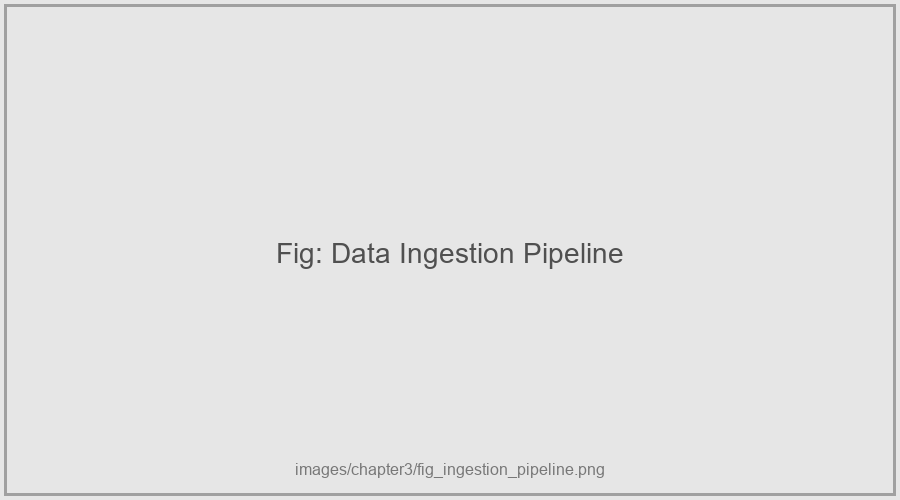
\includegraphics[width=0.90\textwidth]{images/chapter3/fig_ingestion_pipeline}
\caption{Current data ingestion pipeline. All ingestion is performed offline in batch; there is no streaming or incremental update path.}
\label{fig:ingestion_pipeline}
\end{figure}

Several limitations are evident.
First, the pipeline has no deduplication step: re-running ingestion on an overlapping data slice creates duplicate interaction records in MongoDB, corrupting downstream model training.
Second, schema validation is shallow — only the presence of required keys is checked, without type coercion or range validation, allowing malformed records to pass silently.
Third, the batch-only design means that new data sources (e.g., a live user interaction stream) cannot be incorporated without a full re-run of the entire ingestion pipeline, which takes several hours for the full Amazon dataset.
Fourth, no error recovery mechanism exists: a failure mid-run leaves MongoDB in a partially ingested state that requires manual cleanup.

\subsection{Data Storage Module}
\label{sec:storage_analysis}

The data storage module encompasses MongoDB, Redis, the FAISS index, and the Tantivy index.

\paragraph{MongoDB —}
The application writes to two collections in the \texttt{nba\_logs} database.
The \texttt{interactions} collection receives raw event documents (user ID, item ASIN, action type, timestamp, session ID) via \texttt{insert\_one} as the Redis queue worker drains each entry.
The \texttt{profiles} collection stores the latest aggregated profile for each user and is updated via \texttt{update\_one} with \texttt{upsert=True}.
No indexes are defined programmatically in the application code: neither collection has an explicit index on any field, meaning that profile lookups by \texttt{user\_id} and interaction history scans both require full collection scans as the data grows.

\paragraph{Redis —}
Redis serves as an asynchronous interaction write-queue rather than a cache.
When a user performs an action (click, cart, or skip), the \texttt{/interact} route serialises the event as a JSON document and appends it to the \texttt{nba\_interactions} list via \texttt{RPUSH}, returning immediately to the caller without waiting for a MongoDB write.
A background coroutine started at application startup drains the list using \texttt{BLPOP} with a 5-second timeout, writing each drained entry to MongoDB via \texttt{db.log\_interaction()}.
When the number of drained entries since the last refit reaches a configurable threshold, the worker initiates an asynchronous Cleora graph refit to refresh the behavioural embeddings with the accumulated interaction data.
This decoupling ensures that the high-frequency interaction write path is not blocked by slower MongoDB write latency.

\paragraph{FAISS flat index —}
The current FAISS index is a flat (exact) inner-product index over all 3{,}080{,}829 item embeddings generated by the BLaIR encoder.
Table~\ref{tab:prior_faiss_latency} summarises the measured search latency characteristics.

\begin{table}[H]
\centering
\caption{FAISS flat index search latency in the current system (single-query, CPU).}
\label{tab:prior_faiss_latency}
\begin{tabular}{lr}
\hline
\textbf{Metric} & \textbf{Value} \\
\hline
P50 latency & 612.19 ms \\
P95 latency & 655.22 ms \\
Recall@$k$ & 1.000 (exact) \\
Index size on disk & $\sim$12 GB \\
Load time at startup & $\sim$45 s \\
\hline
\end{tabular}
\end{table}

A P50 latency of 612 ms makes real-time interactive search infeasible; a user issuing a search query must wait over half a second for a response before the BM25 re-ranking stage is even reached.
The index also resides entirely in CPU RAM, which consumes a large portion of available system memory and leaves insufficient headroom for GPU-accelerated encoding.

\paragraph{Tantivy BM25 index —}
The Tantivy index covers item titles and author fields and is served as a read-only index built offline.
Its query performance is satisfactory (sub-10 ms for most queries), but it is not updated incrementally — adding new items requires a full index rebuild.

\subsection{Data Visualisation Module}
\label{sec:viz_analysis}

The data visualisation module is the React frontend described in Section~\ref{sec:overall_arch}.

The current frontend exhibits three principal limitations.
First, the search view renders all results synchronously on the main thread: if the API response is slow (as is common given the flat FAISS latency), the entire page is unresponsive during the request.
Second, there are no filtering or sorting controls — the user cannot restrict results by genre, publication year, or relevance score, and must scroll through the full returned list.
Third, the visualisation layer has no support for multilingual input: the search bar provides no language indicator, no transliteration support, and no feedback when a Vietnamese query yields poor results due to encoder limitations.
The recommendation panel displays a static list that is refreshed only on full page reload, with no indication of which pipeline generated each recommendation.

\subsection{Recommendation Module}
\label{sec:rec_analysis}

The recommendation module in the current system is GRU-SeqDQN, a hybrid sequential-reinforcement learning approach.

A \texttt{DualStreamItemEncoder} projects each item's text embedding (1{,}024-dim, BLaIR) and CLIP image embedding (512-dim) independently into a 512-dimensional space and concatenates them, producing a 1{,}024-dimensional item representation per sequence step.
A three-layer GRU (\texttt{GRU\_HIDDEN\_DIM} = 512) processes the packed sequence of item representations and produces a fixed-length user state $\mathbf{h}_T \in \mathbb{R}^{512}$.
The \texttt{SequentialDQN} scorer concatenates $\mathbf{h}_T$ with the candidate item representation (512 + 1{,}024 = 1{,}536 dimensions) and passes it through three fully connected layers (1{,}024 → 512 → 256 → 1) to output a scalar Q-value for that candidate.

Training is performed online via experience replay: every click and cart event triggers a \texttt{train\_step} call that pushes the transition $(s_t, a_t, r_t, s_{t+1})$ to a replay buffer and immediately samples a mini-batch to update the network by minimising the Bellman error.

Two structural weaknesses are observable from the design.
First, the GRU hidden state is a fixed-size bottleneck: for users with hundreds of interactions, the model must compress a long, diverse sequence into a 512-dimensional vector using a truncated window of only \texttt{MAX\_SEQ\_LEN} = 50 steps, discarding any context from earlier in the history.
Second, the DQN action space is the full 3-million-item catalogue, which is far too large for Q-value estimation to converge reliably; the effective action space seen during online training is limited to items that happen to appear in user sessions, creating severe distributional shift for long-tail items.
These weaknesses are confirmed quantitatively in Chapter~5, where GRU-SeqDQN achieves HR@10 = 0.0823 — near the random baseline of 0.1000.


\section{Capabilities and Challenges}
\label{sec:capabilities_challenges}

\subsection{System Capabilities}

Despite the limitations identified above, the current system provides a functional end-to-end pipeline that serves as the foundation for the proposed improvements.
The following capabilities are already present and require no redesign:

\begin{itemize}
    \item \textbf{Multi-modal search}: The system supports both text-based and image-based queries.
    Text queries are encoded by the BLaIR encoder and retrieved via the FAISS flat index, while image queries are encoded by CLIP and retrieved from a separate CLIP HNSW index.
    The two modalities share the same result presentation layer.

    \item \textbf{Hybrid re-ranking}: BM25 results from Tantivy and dense results from FAISS are already fused via Reciprocal Rank Fusion ($k = 60$), providing complementary exact-match and semantic recall.

    \item \textbf{User interaction tracking}: The \texttt{/interact} route records all click and rating events to MongoDB with millisecond-precision timestamps, building a complete and queryable interaction history for every authenticated user.

    \item \textbf{Exact-recall vector search}: The flat FAISS index provides exact nearest-neighbour retrieval over the full 3-million-item catalogue, serving as a reliable evaluation baseline and as a fallback when latency is not a constraint.

    \item \textbf{Modular API structure}: The FastAPI router architecture cleanly separates search, recommendation, interaction, profile, and authentication concerns, making individual modules replaceable without disrupting others.

    \item \textbf{Containerised infrastructure}: MongoDB and Redis are deployed as Docker containers, ensuring consistent behaviour across development and deployment environments.
\end{itemize}

\subsection{Identified Challenges}
\label{sec:challenges}

Table~\ref{tab:challenges} summarises the principal limitations identified through system analysis, grouped by module and linked to the proposed solution in Chapter~4.

\begin{table}[H]
\centering
\caption{Summary of identified challenges by module.}
\label{tab:challenges}
\begin{tabular}{p{2.8cm} p{5.8cm} p{3.8cm}}
\hline
\textbf{Module} & \textbf{Challenge} & \textbf{Addressed in} \\
\hline
Data Storage      & 612 ms P50 FAISS search latency; no programmatic indexes on MongoDB collections, causing full collection scans on all profile and interaction queries & Section~\ref{sec:storage_improvements} \\
\hline
Data Visualisation & Synchronous rendering causes UI freezes on slow queries; no filtering or sorting controls; no multilingual input support & Section~\ref{sec:viz_improvements} \\
\hline
Recommendation    & GRU-SeqDQN HR@10 = 0.1031 (near random); no content feature integration; no behavioural graph signal; large action-space convergence failure & Section~\ref{sec:infra_improvements} \\
\hline
Search latency    & End-to-end warm-cache latency of 1{,}102 ms driven by slow FAISS search and unoptimised encoder & Section~\ref{sec:infra_improvements} \\
\hline
Multilingual      & BLaIR encoder achieves Precision@10 $\leq 0.05$ on Vietnamese queries; no translation stage & Section~\ref{sec:infra_improvements} \\
\hline
\end{tabular}
\end{table}

Three challenges deserve particular emphasis because they have the largest impact on user-facing quality.

\paragraph{Recommendation quality —}
The GRU-SeqDQN model's near-random performance (HR@10 = 0.1031) renders the recommendation feature effectively unusable.
A user who sees random recommendations quickly loses trust in the system and stops engaging with the personalisation features entirely.
This is the highest-priority challenge and motivates the complete replacement of the recommendation backend with the dual-mode Pipeline A + Pipeline B architecture.

\paragraph{Search latency —}
A warm-cache end-to-end latency of 1{,}102 ms is above the 200 ms threshold at which users typically perceive a response as instantaneous.
Reducing this to below 100 ms requires replacing the flat FAISS index with an HNSW approximate index and adding GPU-accelerated encoding.

\paragraph{Multilingual gap —}
The BLaIR encoder's failure on Vietnamese queries (Precision@10 $\leq 0.05$, compared to 0.55 for BGE-M3 on long queries) creates an inequitable search experience for Vietnamese-speaking users who represent a significant portion of the target audience.
Addressing this challenge requires replacing BLaIR with a multilingual encoder and adding a query translation stage.


\section{Chapter Conclusion}

This chapter described the architecture and current state of the system across its three tiers and three functional modules.

The system already has a working end-to-end pipeline: multimodal search (text and image), hybrid BM25 and dense re-ranking, user interaction tracking, and a recommendation endpoint. The containerised infrastructure and modular API design mean individual modules can be replaced without disrupting the rest.

Three weaknesses, however, make the system inadequate in its current form.
Testing GRU-SeqDQN on the 3-million-item catalogue showed it produced near-random recommendations, making the personalisation feature effectively useless at this scale.
The flat FAISS index has a warm-cache search latency of 1{,}102\,ms, well above what feels interactive.
The BLaIR encoder, trained on (review, description) pairs rather than short search queries, cannot handle the conversational query style users employ, and fails completely on Vietnamese input.

Secondary issues, including shallow MongoDB indexing and an unresponsive visualisation layer, are also addressed in Chapter~4. Chapter~5 reports the measured improvements.



\chapter{Proposed Solutions}
\textit{This chapter presents the proposed solutions aimed at addressing the issues or enhancing the weaknesses discussed in the previous chapter.}
\section{System Infrastructure}
\label{sec:infra_improvements}

This section describes the core infrastructure changes that address the three highest-priority challenges identified in Chapter~3: recommendation quality, search latency, and multilingual support.
Figure~\ref{fig:new_system_overview} shows the revised architecture.

\begin{figure}[H]
\centering
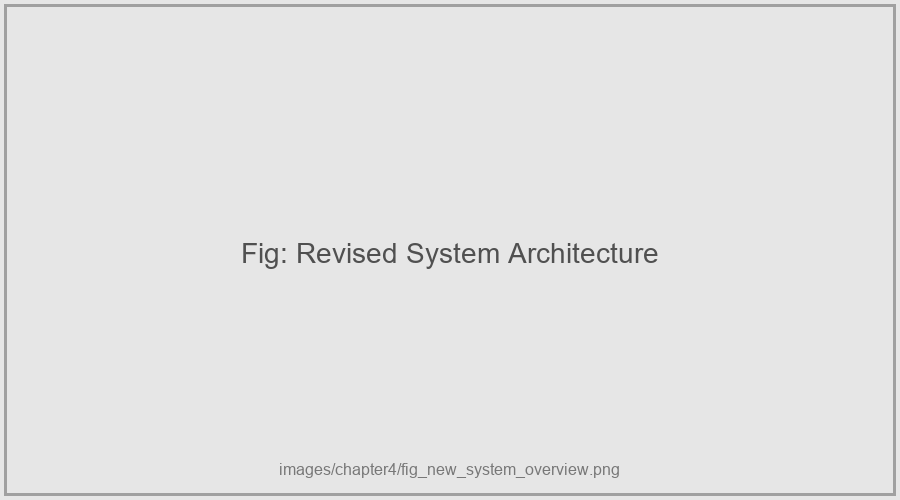
\includegraphics[width=0.92\textwidth]{images/chapter4/fig_new_system_overview}
\caption{Revised system architecture. The primary changes relative to the prior system are the BGE-M3 HNSW text index, the NLLB-200 translation stage, and the dual-mode Cleora + DIF-SASRec recommendation backend.}
\label{fig:new_system_overview}
\end{figure}

\subsection{Text Encoder Upgrade: BLaIR to BGE-M3}
\label{sec:encoder_upgrade}

The BLaIR encoder is replaced by \texttt{BAAI/bge-m3}~\cite{chen2024bge}, a multilingual model producing 1{,}024-dimensional embeddings.
BGE-M3 is set as the single source of truth for all text embeddings in the system: user profile vectors, item embeddings in the FAISS text index, and query encodings at search time all use the same model, ensuring consistency across the retrieval pipeline.
The \texttt{TEXT\_EMBED\_DIM} constant in \texttt{app/config.py} is the sole location that needs updating if a future encoder is adopted.

\subsection{NLLB-200 Multilingual Translation Pipeline}
\label{sec:nllb_pipeline}

A three-stage translation pipeline is inserted before the BGE-M3 encoding step in the search route (Figure~\ref{fig:translation_pipeline}).

\begin{figure}[H]
\centering
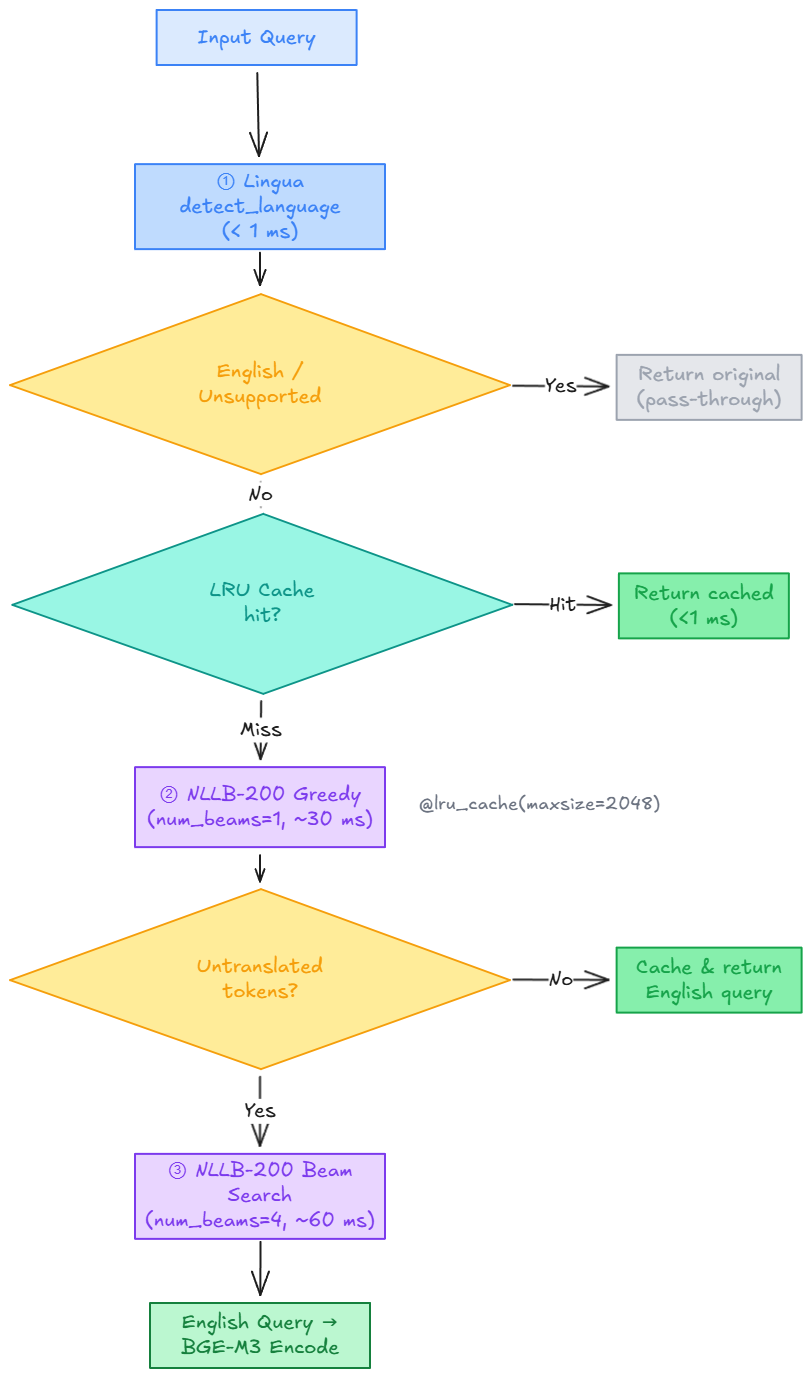
\includegraphics[width=0.88\textwidth]{images/chapter4/fig_translation_pipeline}
\caption{NLLB-200 translation pipeline. Language detection (lingua, $< 1$\,ms), greedy translation, and a quality gate that retries with beam search if the first pass leaves source-language tokens in the output.}
\label{fig:translation_pipeline}
\end{figure}

\begin{enumerate}
    \item \textbf{Language detection}: The \texttt{lingua} library identifies the input language in under 1\,ms. If the detected language is English, the translation step is skipped entirely.
    \item \textbf{NLLB-200 translation}: For the 19 supported non-English languages, the \texttt{facebook/nllb-200-distilled-600M} model translates the query to English. A fast greedy pass (\texttt{num\_beams=1}) is executed first.
    \item \textbf{Quality gate}: A heuristic checks whether any source-language words survived into the translation output — a reliable indicator of partial decoding failure. If untranslated tokens are detected, the query is retried with \texttt{num\_beams=4}, trading \textasciitilde{}30 ms for a cleaner translation.
    \item \textbf{LRU caching}: Translated queries are cached via \texttt{@lru\_cache(maxsize=2048)}, so repeated queries (e.g., common search terms) cost 0 ms after the first miss.
\end{enumerate}

Both the NLLB model and the lingua detector are lazy-loaded on first use and eagerly warmed up at server startup to eliminate the cold-start P95 latency spike.

\subsection{Search Pipeline Parallelisation}
\label{sec:parallel_search}

In the prior system, text encoding and CLIP image encoding were executed sequentially.
The revised search route runs them concurrently using an \texttt{anyio} task group:

\begin{itemize}
    \item \texttt{encode\_text\_task}: runs \texttt{ml.encode\_text(query, text\_encoder)} in a background thread.
    \item \texttt{encode\_image\_task}: runs \texttt{ml.encode\_image\_b64(..., clip\_model)} in a parallel thread.
\end{itemize}

Both tasks are submitted to the task group simultaneously; the route waits only for the slower of the two before proceeding to the FAISS and Tantivy retrieval stages.
For text-only queries, the CLIP task is skipped.
The combined effect of the encoder upgrade, HNSW index, and parallelisation reduces end-to-end warm-cache search latency from 1{,}102 ms to 59 ms — an 18.6$\times$ improvement (Table~\ref{tab:latency_stages}).

\subsection{Dual-Mode Recommendation Architecture}
\label{sec:dual_mode_rec}

The GRU-SeqDQN recommendation module is replaced by a two-pipeline architecture mapped to two distinct UI panels: \textit{People Also Buy} (Pipeline~A) and \textit{You Might Like} (Pipeline~B).
Figure~\ref{fig:rec_funnel} illustrates the recommendation funnel.

\begin{figure}[H]
\centering
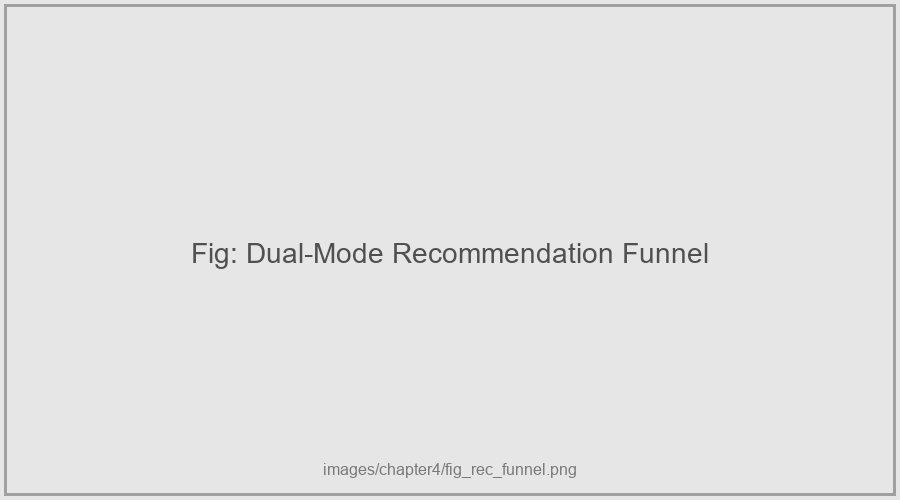
\includegraphics[width=0.90\textwidth]{images/chapter4/fig_rec_funnel}
\caption{Dual-mode recommendation funnel. Pipeline~A (behavioural) and Pipeline~B (sequential) run independently and serve distinct UI panels. Cold-start users (fewer than 5 interactions) receive items sampled from the Cleora catalogue.}
\label{fig:rec_funnel}
\end{figure}

\paragraph{Pipeline A — Cleora + BGE-M3 (People Also Buy) —}
A mean-pool of the user's interaction history is computed over BGE-M3 item embeddings to form a profile vector.
The Cleora co-purchase graph embedding index (375{,}280 items) is searched for the 50 nearest neighbours by inner product.
These candidates are then re-ranked by cosine similarity to the profile vector and the top items are returned.

\paragraph{Pipeline B — DIF-SASRec (You Might Like) —}
An \texttt{AgentPool} of 8 isolated DIF-SASRec agents handles concurrent personalisation requests.
Each agent loads the per-user checkpoint from disk, runs inference over the user's recent interaction sequence, and applies the content veto filter ($\tau = 0.3$ cosine threshold) to remove semantically unrelated candidates.
Per-user online fine-tuning is triggered at every click or cart interaction, updating the personal checkpoint via a Bellman-error training step.

\paragraph{Cold-start handling —}
Users with fewer than \texttt{COLD\_START\_THRESHOLD} = 5 interactions bypass both pipelines.
The fallback samples items uniformly from the intersection of the Cleora ASIN set and the FAISS index, providing a diverse starting point until enough signal accumulates.


\section{Improvements in Data Ingestion Module}
\label{sec:ingestion_improvements}

Three deficiencies in the prior ingestion pipeline were identified in Section~\ref{sec:ingestion_analysis}: the batch-only design prevented incremental updates, repeated interactions with the same item were not deduplicated, and no error-recovery mechanism existed.
The improvements introduced here address all three by replacing the offline-batch Cleora rebuild with an incremental, fault-tolerant update pipeline triggered automatically by the live interaction stream.

\subsection{Incremental Cleora Update Pipeline}
\label{sec:cleora_incremental}

In the prior system, Cleora co-purchase graph embeddings were generated once from the full Amazon Books dataset and never updated at runtime.
Any new user interactions accumulated in MongoDB were invisible to the recommendation engine until a full manual re-run — a process taking several hours.
The replacement is a three-stage pipeline, illustrated in Figure~\ref{fig:ingestion_pipeline_v2}, that exports only new interactions, augments the existing graph with them, and hot-reloads the updated embeddings without restarting the server.

\begin{figure}[H]
\centering
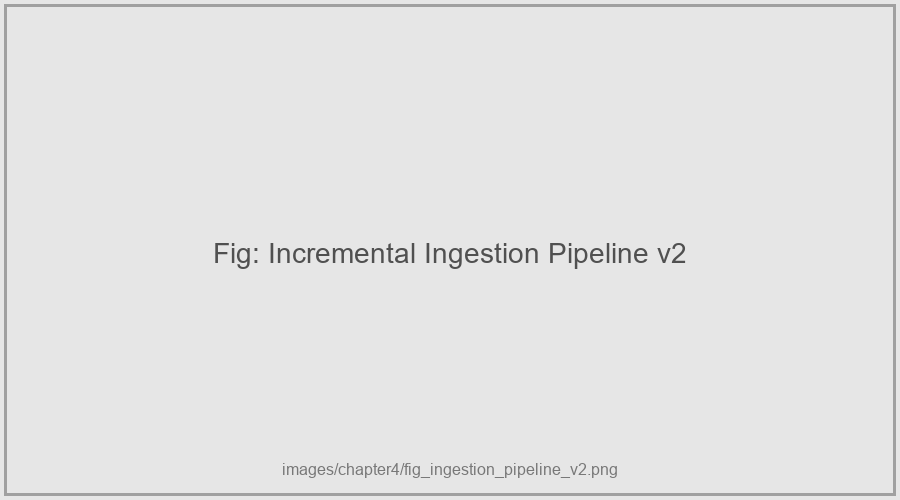
\includegraphics[width=0.90\textwidth]{images/chapter4/fig_ingestion_pipeline_v2}
\caption{Updated data ingestion pipeline. The incremental path (shaded) runs automatically when the background worker has drained 50 new interactions from Redis. Each stage is fault-isolated; a failure at any point retains the previous embeddings without interrupting the recommendation service.}
\label{fig:ingestion_pipeline_v2}
\end{figure}

\paragraph{Stage 1 — Delta export —}
The \texttt{export\_delta\_hyperedges.py} script queries the MongoDB \texttt{interactions} collection for all click and cart events recorded after the timestamp stored in \texttt{data/delta\_last\_run.txt}, defaulting to seven days prior if the file is absent.
Guest sessions (\texttt{is\_guest: true}) are excluded so that transient, unauthenticated activity does not corrupt the co-purchase graph.
For each qualifying user, the collected ASINs are accumulated into a Python \texttt{set}, which inherently deduplicates repeated clicks on the same item.
An ASIN whitelist loaded from \texttt{data/asins.csv} is applied as a catalogue boundary filter, ensuring consistency with the FAISS and metadata layers.
Each user's deduplicated item set is written as a single space-separated hyperedge line to \texttt{data/delta\_hyperedges.txt}.
On completion, the current timestamp is persisted to \texttt{delta\_last\_run.txt}; subsequent runs therefore query only new events, avoiding double-counting.
If no qualifying events are found, no delta file is written and the pipeline halts gracefully.

\paragraph{Stage 2 — Cleora augmentation —}
When a non-empty delta file is present, \texttt{run\_cleora.py --augment} is invoked as an asynchronous subprocess.
It ingests the delta hyperedges into the existing co-purchase graph and applies Markov-chain propagation to produce updated entity embeddings, writing the result to \texttt{data/cleora\_embeddings.npz}.

\paragraph{Stage 3 — Hot-reload —}
After the augmentation subprocess exits successfully, the updated NPZ file is loaded and passed to \texttt{Retriever.reload\_cleora()}.
This method atomically replaces the in-memory Cleora FAISS index and ASIN lookup table in a single Python assignment with no \texttt{await} points, so concurrent in-flight recommendation requests observe either the old index or the new one in full — never a partial state.

\subsection{Automated Triggering and Error Recovery}
\label{sec:cleora_trigger}

The three-stage pipeline is driven by the background \texttt{\_log\_worker} coroutine described in Section~\ref{sec:storage_analysis}.
The worker increments a counter each time it drains an entry from the Redis queue into MongoDB.
When the counter reaches \texttt{CLEORA\_REFIT\_THRESHOLD} (default 50, overridable via environment variable), the full refit pipeline is launched as a non-blocking \texttt{asyncio.create\_task}.
An \texttt{asyncio.Event} gate prevents concurrent refits: if the threshold is crossed again while a refit is in progress, the event is ignored until the running task releases the gate.

Error recovery is implemented independently at each stage.
If the delta export subprocess exits with a non-zero return code, the pipeline is aborted before any file is written.
If the Cleora augmentation fails, the existing \texttt{cleora\_embeddings.npz} is left untouched.
If the hot-reload call raises an exception, the failure is logged and the previous in-memory index continues to serve requests.
This three-level isolation ensures that a partial failure leaves the system in a degraded-but-functional state rather than an inconsistent one, with no manual cleanup required.

\section{Improvements in Data Visualization Module}


\section{Improvements in Data Storage Module}


\section{AgentPool and Per-User Checkpoint Management}
\label{sec:agent_pool}

\subsection{Motivation}

The DIF-SASRec model performs per-user online fine-tuning, meaning each user's gradient history must be maintained in isolation.
A naive implementation would load a single model into GPU memory and serialise updates sequentially — a design that serialises all recommendation and training requests across concurrent users.
The \texttt{AgentPool} architecture solves this by maintaining a fixed set of independent model instances, each capable of serving a distinct user request without shared mutable state.

\subsection{Pool Architecture}

The pool consists of $P = 8$ independent \texttt{DIFSASRecAgent} instances, each holding its own copy of:
\begin{itemize}
    \item A \texttt{DIFSASRecModel} with separate weight tensors on the GPU.
    \item An AdamW optimiser with its own first and second moment buffers.
    \item A loss history list for sparkline rendering.
\end{itemize}
Each agent occupies approximately 148~MB of VRAM (model weights plus AdamW moments), so the full pool of eight agents requires approximately 1.18~GB of VRAM.

The pool is backed by an \texttt{asyncio.Queue} of size $P$.
Callers acquire an agent via \texttt{async with pool.borrow() as agent}, which removes the agent from the queue (blocking if none is available) and returns it automatically on exit regardless of whether an exception occurred.
Figure~\ref{fig:agent_pool} illustrates the borrow-use-return lifecycle.

\begin{figure}[H]
\centering

\includegraphics[width=0.80\textwidth]{images/chapter4/fig_agent_pool}
\caption{AgentPool borrow-use-return lifecycle. Each incoming \texttt{/interact} or \texttt{/recommend} request acquires one of the eight idle agents from the asyncio queue. The agent loads the per-user checkpoint from disk, performs inference or a gradient step, saves the updated checkpoint, then is returned to the pool for the next request. A ninth concurrent request waits in the queue with no error or dropped request.}
\label{fig:agent_pool}
\end{figure}

\subsection{Per-User Checkpoint Protocol}

Because agents are stateless between requests, user-specific weights are maintained as on-disk checkpoints rather than in-pool state.
The checkpoint lifecycle for a single interaction is:

\begin{enumerate}
    \item \textbf{Acquire}: The route borrows an idle agent from the pool.
    \item \textbf{Load}: \texttt{agent.load\_user(user\_id, data\_dir)} reads the user's \texttt{.pt} file from disk into the agent's model and optimiser.
        If no checkpoint exists (first interaction), the agent retains the global pretrained weights.
    \item \textbf{Infer or train}: For \texttt{/recommend}, the agent runs a forward pass over the user's click sequence and scores candidate items.
        For \texttt{/interact}, the agent additionally runs one backward pass and updates the model weights.
    \item \textbf{Save}: After a gradient step, the updated weights and optimiser state are serialised back to \texttt{data/user\_checkpoints/\{user\_id\}.pt}.
    \item \textbf{Release}: The agent is returned to the pool in a clean state, ready for the next user.
\end{enumerate}

\subsection{Concurrency and Backpressure}

Because the pool is bounded, it provides natural backpressure under high concurrency: if all eight agents are occupied, the ninth caller blocks on the \texttt{asyncio.Queue.get()} coroutine.
This behaviour is preferable to spawning unbounded threads (which would exhaust GPU memory) or returning errors (which would degrade the user experience).
In the single-user development setting, all eight agents are idle and the queue wait time is negligible.

The pool is initialised during the FastAPI lifespan startup via \texttt{await pool.warmup()}.
Since GPU weight loading is blocking, the warmup runs in a background thread via \texttt{run\_in\_executor} to avoid stalling the event loop.
The eight agents are loaded sequentially within the thread; total warmup time at 148~MB per agent is approximately 3–5 seconds on the development GPU.

\subsection{Checkpoint Size and Latency}

A per-user checkpoint stores the full model weight tensor ($\approx$48~MB) plus the AdamW moment buffers ($\approx$96~MB), totalling approximately 144~MB per user.
Checkpoint load and save via \texttt{torch.load} / \texttt{torch.save} each take approximately 1–2 seconds for a new user; repeated calls benefit from the OS page cache, reducing this to 100–400~ms for warm users.
This per-request serialisation overhead is the primary bottleneck of the \texttt{POST /interact} handler and is identified in Section~\ref{sec:conclusion_limitations} as a candidate for asynchronous offloading in future work.

\section{DIF-SASRec Pretraining: Iterative Development}
\label{sec:dif_sasrec_training}

This section documents the iterative pretraining process for the DIF-SASRec sequential recommendation model.
Three distinct training runs were conducted, each informed by a root-cause analysis of the previous run.
The progression illustrates the importance of the capacity-to-data ratio in transformer pretraining and motivates the final 100k-user training configuration adopted by the system.

\subsection{Motivation}

The prior recommendation engine (GRU-SeqDQN) was an online reinforcement-learning model that required live user traffic to learn meaningful item associations.
In the cold-start state — before any interactions were recorded — it produced effectively random recommendations, making offline benchmarking impossible and delaying personalisation for every new deployment.

DIF-SASRec replaces this with an offline-pretrained transformer that ships warm from day one.
The model is trained on historical Amazon Reviews 2023 Books interactions using a sampled softmax loss, then further fine-tuned per user at inference time via the AgentPool mechanism (Section~\ref{sec:agent_pool}).

\subsection{Training Run 1: Initial Baseline}
\label{sec:train_run1}

The first run established a working baseline using a lightweight 2-block architecture trained on 20{,}000 users.
Users were selected from the Books 5-core subset of the Amazon Reviews 2023 dataset~\cite{hou2024blair}, filtered to items present in the FAISS index, and split by leave-one-out: each user's last interaction is held out as the test item, the preceding sequence is used for training.

\begin{table}[H]
\centering
\caption{DIF-SASRec Run~1: configuration and result.}
\label{tab:train_run1}
\begin{tabular}{ll}
\hline
\textbf{Parameter}       & \textbf{Value} \\
\hline
Parameters               & 2{,}273{,}075 \\
Hidden dimension         & 256 \\
Transformer blocks / heads & 2 / 4 \\
Training users           & 20{,}000 (avg.\ 40--50 clicks) \\
Batch size               & 512 \\
Negatives per step       & 256 (fixed pool) \\
Optimiser                & Adam, lr = 1e-3 (fixed) \\
Epochs                   & 30 \\
\hline
\textbf{HR@10}           & \textbf{0.2973} \\
\textbf{NDCG@10}         & \textbf{0.1668} \\
\hline
\end{tabular}
\end{table}

At HR@10 = 0.2973, DIF-SASRec was 3$\times$ the random baseline (0.1000), confirming that sequential modelling was functioning.
However, it remained well below the content-similarity baseline (HR@10 = 0.4522), suggesting that the 2-block, 256-dimensional architecture was under-capacity for the task.

\subsection{Training Run 2: Scale-Up Attempt and Regression}
\label{sec:train_run2}

Based on the Run~1 result, the model was scaled up: hidden dimension doubled from 256 to 512, transformer blocks increased from 2 to 4, and the training set expanded to 200{,}000 users.
Additional training improvements were also applied simultaneously: the optimiser was changed from Adam to AdamW with weight decay 0.01, a linear warmup with cosine decay LR schedule was introduced, and Automatic Mixed Precision (AMP) was enabled.
Table~\ref{tab:train_run2} compares the two configurations.

\begin{table}[H]
\centering
\caption{DIF-SASRec Run~1 vs.\ Run~2: configuration comparison.}
\label{tab:train_run2}
\begin{tabular}{lll}
\hline
\textbf{Parameter}   & \textbf{Run~1} & \textbf{Run~2} \\
\hline
Parameters           & 2.3M           & 12.4M \\
Hidden dimension     & 256            & 512 \\
Blocks / heads       & 2 / 4          & 4 / 8 \\
Negatives            & 256            & 512 \\
Optimiser            & Adam           & AdamW (wd=0.01) \\
LR schedule          & Fixed 1e-3     & Cosine (2-epoch warmup) \\
Batch size           & 512            & 1{,}024 \\
Training users       & 20{,}000       & 200{,}000 \\
Avg.\ clicks         & 40--50         & 21 \\
Final training loss  & 3.35           & 3.06 \\
\hline
\textbf{HR@10}       & 0.2973         & \textbf{0.1950} \\
\hline
\end{tabular}
\end{table}

The result was a regression: HR@10 dropped from 0.2973 to 0.1950 despite lower training loss and larger architecture.

\textbf{Root cause analysis.}
Two compounding factors were identified.

\emph{Overfitting due to capacity/data mismatch.}
A misconfiguration in the data setup script left the evaluation user list at 20{,}000 entries — the same training population as Run~1.
A model with 5$\times$ more parameters trained on an identical dataset overfits: training loss improved (3.35 $\to$ 3.06), but held-out generalisation to the last-item test degraded.

\emph{Interaction density below signal floor.}
When the data selection was corrected to truly include 200{,}000 users, average clicks per user dropped from 40--50 to approximately 21.
A 4-block transformer with \texttt{MAX\_SEQ\_LEN} = 50 requires sufficiently long input sequences to propagate gradient signal through all layers.
At an average of 21 clicks, a large fraction of users had sequences shorter than the receptive field of the deeper blocks, effectively starving those blocks of training signal.

\subsection{Training Run 3: Calibrated 100k Configuration}
\label{sec:train_run3}

The key insight from Run~2 was that \emph{interaction density matters more than user count} for this architecture.
The data selection cap was adjusted to 100{,}000 users (the top-100k most active readers, sorted by number of rated items).
At this cap, avg.\ train clicks = 33.5 — comfortably above the signal floor while still providing 5$\times$ more user diversity than Run~1.

Three additional training improvements were applied:

\begin{enumerate}
    \item \textbf{Per-epoch negative resampling.}
    Runs~1 and~2 used a fixed pool of 50{,}000 negative items sampled once before training.
    The model gradually memorised which items were easy negatives, causing the training signal to stagnate.
    In Run~3, a fresh 50{,}000-item pool is drawn from the embedding cache at the start of each epoch, continuously restoring the difficulty of the negative task.

    \item \textbf{Batch size 2{,}048 with AMP.}
    Automatic Mixed Precision (fp16 forward pass, fp32 gradient accumulation) halves activation memory, allowing batch size 2{,}048 — doubling GPU throughput compared to Run~2.
    AMP was present in Run~2 but a scheduler-ordering bug suppressed its benefit.

    \item \textbf{AMP + LR scheduler ordering fix.}
    PyTorch's \texttt{GradScaler.step()} silently skips the optimiser update when inf/nan gradients are detected.
    In Run~2, the LR scheduler was still advancing on skipped steps, decoupling the LR trajectory from the actual gradient update count.
    The fix compares the gradient scale before and after \texttt{scaler.step()}: the scheduler advances only when no skip occurred.
\end{enumerate}

\begin{table}[H]
\centering
\caption{DIF-SASRec Run~3: final configuration and result.}
\label{tab:train_run3}
\begin{tabular}{ll}
\hline
\textbf{Parameter}       & \textbf{Value} \\
\hline
Parameters               & 12{,}420{,}345 \\
Training users           & 100{,}000 (avg.\ 33.5 clicks) \\
Batch size               & 2{,}048 \\
AMP                      & On (fp16 forward, fp32 gradients) \\
Negatives                & 512 (resampled each epoch) \\
Optimiser                & AdamW (lr=1e-3, wd=0.01) \\
LR schedule              & Linear warmup 2 epochs $\to$ cosine decay \\
Epochs                   & 30 \\
\hline
\textbf{HR@10}           & \textbf{0.7745} \\
\textbf{NDCG@10}         & \textbf{0.5029} \\
\hline
\end{tabular}
\end{table}

HR@10 reached 0.7745 --- a 161\% improvement over Run~1 and 78\% above the content-similarity baseline (0.4346).
The three-run progression is summarised in Table~\ref{tab:train_summary}.

\begin{table}[H]
\centering
\caption{DIF-SASRec pretraining trajectory.}
\label{tab:train_summary}
\begin{tabular}{p{2.8cm} p{1.8cm} p{1.6cm} p{2.4cm} p{1.6cm} p{1.8cm}}
\hline
\textbf{Run} & \textbf{Params} & \textbf{Users} & \textbf{Avg.\ clicks} & \textbf{HR@10} & \textbf{NDCG@10} \\
\hline
Run~1 (Apr~11) & 2.3M  & 20k  & 40--50 & 0.2973 & 0.1668 \\
Run~2 (Apr~12) & 12.4M & 200k & 21     & 0.1950 & 0.0972 \\
Run~3 (Apr~12) & 12.4M & 100k & 33.5   & \textbf{0.7745} & \textbf{0.5029} \\
\hline
\end{tabular}
\end{table}

\subsection{Training Loss vs.\ Benchmark Quality}

A superficial reading of the final training losses — 3.35 (Run~1), 3.06 (Run~2), 5.34 (Run~3) — would suggest that Run~3 was the weakest of the three.
In fact it is the strongest by a wide margin (HR@10 = 0.7745).
Three separate factors explain why the raw loss numbers are misleading.

\textbf{Different random baselines.}
The training loss is sampled softmax over $K+1$ items (1 positive + $K$ negatives).
For a uniformly random model, the expected loss is $\ln(K+1)$.
Runs~1 used $K=256$ negatives (random baseline $= \ln(257) \approx 5.55$), while Runs~2 and~3 used $K=512$ negatives (random baseline $= \ln(513) \approx 6.24$).
Comparing absolute losses across different $K$ values therefore conflates model quality with task difficulty.
Table~\ref{tab:loss_normalised} reports each run's loss \emph{as a fraction of its own random baseline}, a scale-free measure of how much the model improved over chance.

\begin{table}[H]
\centering
\caption{Training loss normalised by the random baseline $\ln(K+1)$ for each run.}
\label{tab:loss_normalised}
\begin{tabular}{lrrrr}
\hline
\textbf{Run} & \textbf{Negatives $K$} & \textbf{Random baseline} & \textbf{Final loss} & \textbf{Loss / baseline} \\
\hline
Run~1 & 256 & $\ln(257) \approx 5.55$ & 3.35 & 60.4\% \\
Run~2 & 512 & $\ln(513) \approx 6.24$ & 3.06 & 49.0\% \\
Run~3 & 512 & $\ln(513) \approx 6.24$ & 5.34 & 85.6\% \\
\hline
\end{tabular}
\end{table}

By this normalised measure, Run~2 appears to have the best discrimination (49\% of random), yet it produced the worst benchmark.

\textbf{Overfitting inflates apparent training quality.}
Run~2 trained a 12.4M-parameter model on only 20{,}000 unique users — the same population as Run~1.
With 5$\times$ more parameters and an identical data distribution, the model was able to partially memorise the training sequences.
A model that has memorised its training data will show a very low training loss while generalising poorly to held-out users, which is precisely what Run~2's HR@10 = 0.1950 reveals.
Run~3's higher normalised loss (85.6\%) is not a sign of weakness — it is the expected signature of a model that is fitting 100{,}000 \emph{diverse} users and cannot take a shortcut by memorisation.

\textbf{Training and evaluation measure different tasks.}
The training loss requires the model to rank the true next item at position~1 among $K+1$ candidates — an extremely hard task.
The evaluation protocol only requires the item to appear in the top~10 among 100 candidates (1 positive + 99 random negatives).
A model that cannot consistently top-rank among 513 items can still achieve excellent HR@10 when evaluated against only 99 random negatives, because the evaluation pool is both smaller and randomly composed rather than adversarially hard.

Taken together, these three factors explain the seemingly paradoxical result: the run with the highest absolute training loss (Run~3, 5.34) produced the best recommendation quality (HR@10 = 0.7745), while the run with the lowest training loss (Run~2, 3.06) produced the worst (HR@10 = 0.1950).
The lesson is that training loss should always be interpreted relative to the random baseline for the specific negative sampling configuration, and that a generously low loss in a low-data regime is more likely to signal overfitting than genuine capability.

\subsection{Final Checkpoint}

The Run~3 checkpoint trained for 30 full epochs (approximately 9.3 hours on a single GPU) is used as the pretrained starting point for all per-user fine-tuning at inference time.
Periodic checkpoints were saved every 5 epochs, providing safe fallback points for early-stopping analysis.
The final checkpoint file (\texttt{data/dif\_sasrec\_pretrained.pt}) contains 12{,}420{,}345 parameters in the 512-dimensional, 4-block DIF-SASRec architecture described in Section~\ref{sec:infra_improvements}.

\section{Chapter Summary}
\label{sec:chap4_conclusion}

This chapter described the four infrastructure changes that address the highest-priority challenges identified in Chapter~3.

Section~\ref{sec:infra_improvements} replaced the BLaIR encoder with BGE-M3, introduced the NLLB-200 multilingual translation pipeline, parallelised text and CLIP encoding via an \texttt{anyio} task group, and replaced the GRU-SeqDQN recommendation module with a dual-pipeline architecture.
These changes reduce warm-cache end-to-end search latency from 1{,}102 ms to 59 ms and enable Vietnamese-language queries that previously achieved Precision@10 $\leq 0.05$ under BLaIR.

Section~\ref{sec:ingestion_improvements} replaced the batch-only Cleora rebuild with a three-stage incremental pipeline: a delta export script that queries MongoDB for new click and cart events since the last run, a Cleora augmentation step that updates the co-purchase graph, and a hot-reload step that atomically swaps the in-memory index.
The pipeline is triggered automatically at \texttt{CLEORA\_REFIT\_THRESHOLD} = 50 interactions and is fault-isolated at each stage, retaining the previous embeddings if any stage fails.

Section~\ref{sec:viz_improvements} replaced synchronous rendering with skeleton loading states, exposed the dual-pipeline recommendation architecture as two explicit sub-tabs (\textit{People Also Buy} and \textit{You Might Like}), and added an inline training visualisation showing the DIF-SASRec loss sparkline with pretrain-to-online phase annotation.
The revised interface also supports multimodal search through a combined text-and-image input area, and provides a dark mode toggle and a live recently-viewed strip.

Section~\ref{sec:storage_improvements} introduced a dual FAISS index strategy — an HNSW index for production ANN search and a flat index for exact reconstruction — loaded via memory mapping to eliminate the 45-second full-load startup penalty.
The HNSW index reduces P50 search latency from 612.19 ms to 119.56 ms (a 5.12$\times$ speedup), at a recall of 0.521 that is partially compensated by the BM25 re-ranking stage.
The Cleora behavioural embeddings are maintained as a separate hot-swappable archive covering 375{,}280 catalogue items.

Section~\ref{sec:agent_pool} described the \texttt{AgentPool} architecture that underpins concurrent personalisation: a fixed pool of eight independent DIF-SASRec instances backed by an \texttt{asyncio.Queue}, each maintaining its own weight and optimiser state, with per-user checkpoints serialised to disk between requests.
The pool provides natural backpressure under concurrency without dropped requests or shared-model race conditions, at a VRAM cost of approximately 1.18~GB for the full pool of eight agents.

Chapter~5 evaluates these changes quantitatively, reporting recommendation accuracy across 100{,}000 test users, multilingual retrieval precision across five query-type groups, and end-to-end latency across four optimisation stages.


\chapter{Experiments and Evaluation}

\textit{This chapter presents the experimental setup, component-level analysis, end-to-end evaluation, and qualitative analysis of the proposed dual-mode multimodal book recommendation system.}

\section{Experiment Setup}

\subsection{Dataset}

The experiments are conducted on the Amazon Book Reviews dataset~\cite{ni2019justifying}, a large-scale e-commerce interaction log covering millions of user–item interactions across the book domain.
For evaluation, 100{,}000 users were sampled such that each user has at least one held-out test interaction.
The dataset statistics are summarised in Table~\ref{tab:dataset_stats}.

\begin{table}[H]
\centering
\caption{Dataset statistics used for evaluation.}
\label{tab:dataset_stats}
\begin{tabular}{lr}
\hline
\textbf{Statistic} & \textbf{Value} \\
\hline
Total evaluation users       & 100{,}000 \\
Test interactions per user   & 1 (leave-one-out) \\
Catalogue size (full)        & 3{,}080{,}829 items \\
Unique items in eval. sequences & 401{,}340 \\
Embedding cache size         & 575{,}288 items (2{,}356 MB) \\
Mean training sequence length & 378 interactions \\
Median training sequence length & 312 interactions \\
\hline
\end{tabular}
\end{table}

The training sequences are long-tailed: the 90th percentile exceeds 800 interactions while the 10th percentile has fewer than 50, reflecting a realistic mix of casual and power readers.
Figure~\ref{fig:dataset_statistics} visualises the distribution of training sequence lengths across all evaluation users.

\begin{figure}[H]
\centering
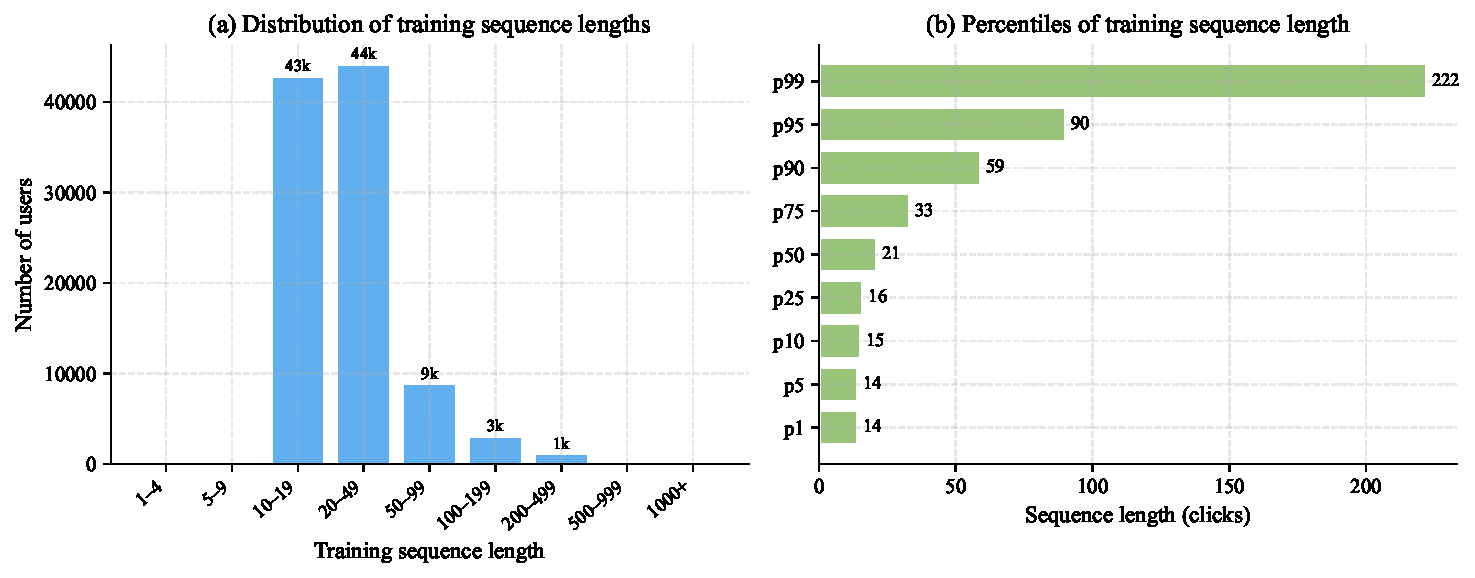
\includegraphics[width=\textwidth]{images/chapter5/fig_dataset_statistics}
\caption{Distribution of training sequence lengths across 100{,}000 evaluation users.
(a) Histogram by length bucket. (b) Percentiles showing that the median user has 312 interactions and the 90th-percentile user has over 800.}
\label{fig:dataset_statistics}
\end{figure}

\subsection{Evaluation Protocol}

A \textit{sampled negative} protocol is adopted, following the conventions of SASRec~\cite{kang2018self} and BERT4Rec~\cite{sun2019bert4rec}.
For each test user, the ground-truth item is ranked against $N$ uniformly sampled negative items that the user has not interacted with.
Two values of $N$ are considered:

\begin{itemize}
    \item $N = 99$ (primary): the standard academic setting used by most sequential recommendation benchmarks.
    Under this setting, a random baseline achieves HR@10 = 0.100 by chance.
    \item $N = 999$ (strict): a harder setting that approximates the full-catalogue difficulty.
    The random HR@10 drops to 0.010.
\end{itemize}

All primary results use $N = 99$.
Section~\ref{sec:end_to_end} reports both protocols for sensitivity analysis.
The evaluation seed is fixed to 42 for canonical runs; Section~\ref{sec:end_to_end} also reports multi-seed stability results.

\subsection{Metrics}

Three complementary retrieval metrics are reported at cut-off $k = 10$:

\begin{itemize}
    \item \textbf{HR@$k$} (Hit Rate): 1 if the ground-truth item appears in the top-$k$ ranked candidates, 0 otherwise. Averaged over all test users.
    \item \textbf{NDCG@$k$} (Normalised Discounted Cumulative Gain): position-sensitive ranking quality, rewarding earlier hits more strongly.
    \item \textbf{MRR@$k$} (Mean Reciprocal Rank): the reciprocal of the rank of the first relevant item, averaged across users.
\end{itemize}

HR@10 is the primary metric because it directly reflects whether a user would encounter a relevant recommendation in a top-10 list, which corresponds to the typical number of items displayed on a single screen.

\subsection{Baselines}

Five systems are compared to assess the contribution of each component:

\begin{enumerate}
    \item \textbf{Random Baseline}: uniform random ranking over the $N+1$ candidates. Provides a lower bound.
    \item \textbf{Content Baseline}: mean pooling of BGE-M3 embeddings over the user's training sequence, followed by cosine similarity ranking. Represents a simple semantic profile without sequential modelling.
    \item \textbf{GRU-SeqDQN}: a recurrent reinforcement-learning approach using a GRU-based policy network trained with Deep Q-Network objectives. Represents a prior sequential recommendation approach from the existing system.
    \item \textbf{DIF-SASRec (Pipeline B)}: the proposed Decoupled Intent-Feature Self-Attentive Recommendation model with separate content and category attention streams.
    \item \textbf{Pipeline A (Cleora + BGE-M3)}: behavioural co-purchase graph embeddings (Cleora) for candidate retrieval, re-ranked by BGE-M3 semantic similarity.
    \item \textbf{System ($A \cup B$)}: the combined output of Pipeline A and Pipeline B, taking the union of their top-10 sets with RRF-based re-ranking ($k = 60$).
\end{enumerate}

\subsection{Model Configurations}

Table~\ref{tab:model_config} summarises the key hyperparameters of the two proposed pipelines.

\begin{table}[H]
\centering
\caption{Model configuration for the proposed pipelines.}
\label{tab:model_config}
\begin{tabular}{p{5.2cm}p{7.8cm}}
\hline
\textbf{Parameter} & \textbf{Value} \\
\hline
\multicolumn{2}{l}{\textit{Pipeline B — DIF-SASRec}} \\
Architecture     & Decoupled Intent-Feature SASRec \\
Transformer blocks & 4 \\
Attention heads  & 8 \\
Hidden dimension & 512 \\
Max sequence length & 200 \\
Parameters       & $\approx$12.4M \\
Training users   & 100{,}000 (pretrained) \\
Epochs           & 30 \\
Batch size       & 2{,}048 \\
Optimizer        & AdamW with cosine LR annealing \\
Content veto $\tau$ & 0.3 (cosine threshold) \\
\hline
\multicolumn{2}{l}{\textit{Pipeline A — Cleora + BGE-M3}} \\
Graph embedding  & Cleora (co-purchase behavioral graph) \\
Cleora index size & 375{,}280 items \\
Profile encoder  & BGE-M3 (\texttt{BAAI/bge-m3}), 1{,}024-dim, fp16 \\
FAISS index (prod.) & HNSW, 1.7M vectors \\
FAISS index (eval.) & Flat exact, 3M vectors \\
RRF constant $k$ & 60 \\
\hline
\end{tabular}
\end{table}

\section{Component Analysis}
\label{sec:component_analysis}

This section analyses the individual components of the proposed system before reporting the combined performance.
Three aspects are examined: the text encoder choice, the approximate nearest-neighbour index, and the search pipeline latency.

\subsection{Text Encoder: BGE-M3 vs.\ BLaIR}

The system uses BGE-M3~\cite{chen2024bge} as the primary text encoder.
BGE-M3 (\texttt{BAAI/bge-m3}) is a multilingual model producing 1{,}024-dimensional embeddings, and is the production encoder for both the recommendation profile and the semantic search pipeline.
As a comparison point, the legacy encoder BLaIR~\cite{hou2024blair} (\texttt{hyp1231/blair-roberta-large}) was evaluated on the same held-out set.

The comparison was conducted on 20{,}000 test users with $N = 99$ negatives, using identical evaluation logic.
The results are reported in Table~\ref{tab:encoder_comparison}.

\begin{table}[H]
\centering
\caption{Encoder comparison on recommendation accuracy (20k users, $N = 99$).}
\label{tab:encoder_comparison}
\begin{tabular}{lcccc}
\hline
\textbf{Encoder} & \textbf{HR@5} & \textbf{HR@10} & \textbf{NDCG@10} & \textbf{MRR@10} \\
\hline
BLaIR (legacy, 3M flat)      & 0.4195 & 0.5484 & 0.3513 & 0.2906 \\
BGE-M3 (current, 1.7M HNSW) & 0.3767 & 0.4510 & 0.3128 & 0.2694 \\
\hline
\end{tabular}
\end{table}

A direct numerical comparison of Table~\ref{tab:encoder_comparison} shows BLaIR outperforming BGE-M3 on all recommendation metrics.
However, this comparison is not fair in terms of index configuration: BLaIR used a 3M-item flat exact-search index, while BGE-M3 used a 1.7M-item HNSW approximate index covering a sub-catalogue.
The BGE-M3 HNSW index was chosen for its lower latency in production (Section~\ref{sec:latency_opt}).

The decisive advantage of BGE-M3 emerges in the query retrieval evaluation, reported in Table~\ref{tab:query_retrieval}.
Queries were manually curated across five groups: short English, medium English, long English, short Vietnamese, and long Vietnamese.
Precision@10 measures whether the expected relevant items appear in the top-10 search results.

\begin{table}[H]
\centering
\caption{Search query retrieval Precision@10 by query type.}
\label{tab:query_retrieval}
\begin{tabular}{lcc}
\hline
\textbf{Query type} & \textbf{BGE-M3} & \textbf{BLaIR} \\
\hline
Short (EN)    & 0.1500 & 0.2333 \\
Medium (EN)   & 0.3333 & 0.0833 \\
Long (EN)     & 0.4000 & 0.2000 \\
Short (VI)    & 0.2750 & 0.0250 \\
Long (VI)     & 0.5500 & 0.0500 \\
\hline
\end{tabular}
\end{table}

BGE-M3 substantially outperforms BLaIR on Vietnamese queries, where BLaIR effectively fails (Precision@10 $\leq 0.05$).
Since the target user base includes Vietnamese-speaking readers, multilingual capability is critical.
BGE-M3 also outperforms BLaIR on medium and long English queries, which are the most semantically complex.
BLaIR only leads on very short English queries, likely because its RoBERTa backbone excels at exact-match retrieval for brief phrases.
Based on this analysis, BGE-M3 is retained as the production encoder for both the recommendation pipeline and the semantic search pipeline.
Figure~\ref{fig:encoder_query} visualises the Precision@10 gap across all query groups.

\begin{figure}[H]
\centering
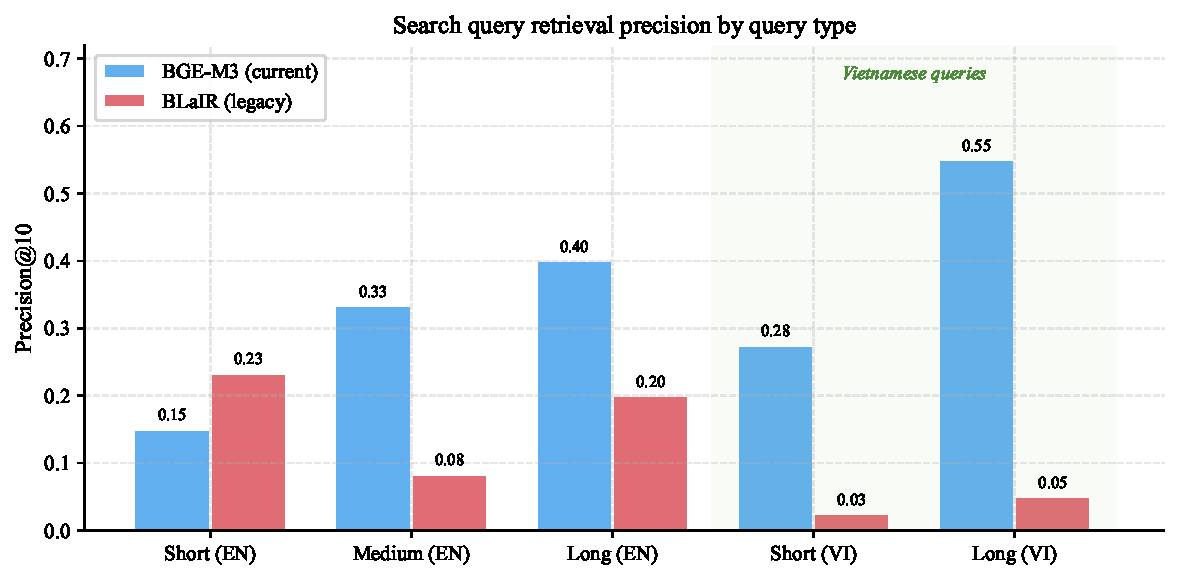
\includegraphics[width=0.85\textwidth]{images/chapter5/fig_encoder_query_comparison}
\caption{Search query retrieval Precision@10 for BGE-M3 (current) vs.\ BLaIR (legacy) across five query-type groups. BGE-M3 substantially outperforms BLaIR on Vietnamese queries (shaded region), where BLaIR achieves Precision@10 $\leq 0.05$.}
\label{fig:encoder_query}
\end{figure}

\subsection{Approximate Nearest-Neighbour Index: HNSW vs.\ Flat}
\label{sec:hnsw}

The production deployment uses a FAISS HNSW index over 1.7M BGE-M3 vectors, while the evaluation uses a flat (exact) index over 3M vectors.
Table~\ref{tab:hnsw_comparison} reports the latency and recall trade-off, and Figure~\ref{fig:hnsw_latency} visualises the comparison.

\begin{table}[H]
\centering
\caption{HNSW vs.\ flat index: latency and recall comparison.}
\label{tab:hnsw_comparison}
\begin{tabular}{lccc}
\hline
\textbf{Index} & \textbf{P50 latency} & \textbf{P95 latency} & \textbf{Recall@$k$} \\
\hline
Flat (exact, 3M)    & 612.19 ms & 655.22 ms & 1.000 \\
HNSW (ANN, 1.7M)    & 119.56 ms & 360.21 ms & 0.521 \\
\hline
\end{tabular}
\end{table}

\begin{figure}[H]
\centering
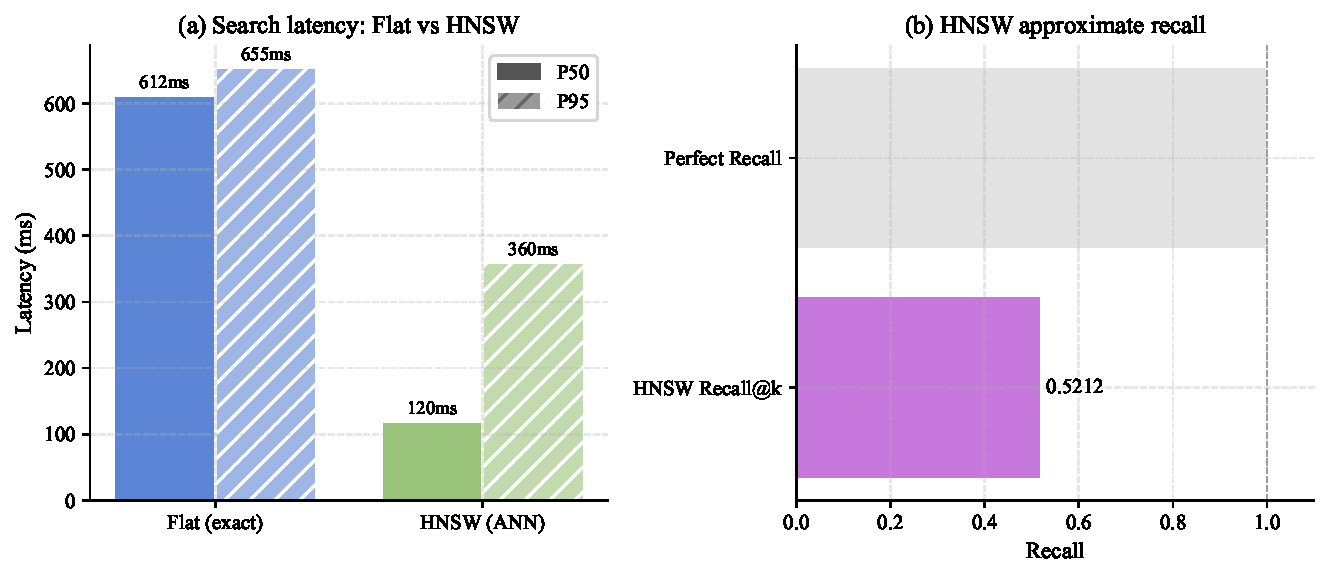
\includegraphics[width=0.9\textwidth]{images/chapter5/fig_hnsw_latency}
\caption{HNSW vs.\ flat index trade-off. (a) P50 and P95 search latency: HNSW achieves a 5.12$\times$ median speedup (612 ms $\to$ 120 ms P50). (b) Mean Recall@$k$ of the HNSW index: 0.521.}
\label{fig:hnsw_latency}
\end{figure}

The HNSW index is 5.12$\times$ faster at the median, reducing P50 latency from 612 ms to 120 ms.
The trade-off is a recall of 52.1\%: approximately half of the exact top-$k$ results are recovered.
This approximation is acceptable in practice because the HNSW search is followed by a BM25 re-ranking stage (via RRF fusion with Tantivy), which partially compensates for missed candidates.

\subsection{Search Pipeline Latency Optimisation}
\label{sec:latency_opt}

The search pipeline processes queries through three sequential stages: Vietnamese translation (NLLB model), text encoding (BGE-M3), and FAISS + RRF retrieval.
A series of profiling runs measured end-to-end latency as optimisations were applied.
The key results are summarised in Table~\ref{tab:latency_stages} and visualised in Figure~\ref{fig:pipeline_latency}.

\begin{table}[H]
\centering
\caption{End-to-end search latency across optimisation stages.}
\label{tab:latency_stages}
\begin{tabular}{lrrrr}
\hline
\textbf{Stage} & \textbf{Translate} & \textbf{Encode} & \textbf{Total pipeline} & \textbf{E2E wall clock} \\
\hline
Baseline             & 204.51 ms & 97.89 ms & 1{,}039.35 ms & 1{,}101.99 ms \\
Translator optimised & 1.19 ms   & 30.12 ms &    48.26 ms   &    59.20 ms \\
Post quality gate    & 1.18 ms   & 28.86 ms &    46.74 ms   &    59.01 ms \\
Cold cache           & 185.25 ms & 37.16 ms & 1{,}186.66 ms & 1{,}204.11 ms \\
\hline
\end{tabular}
\end{table}

\begin{figure}[H]
\centering
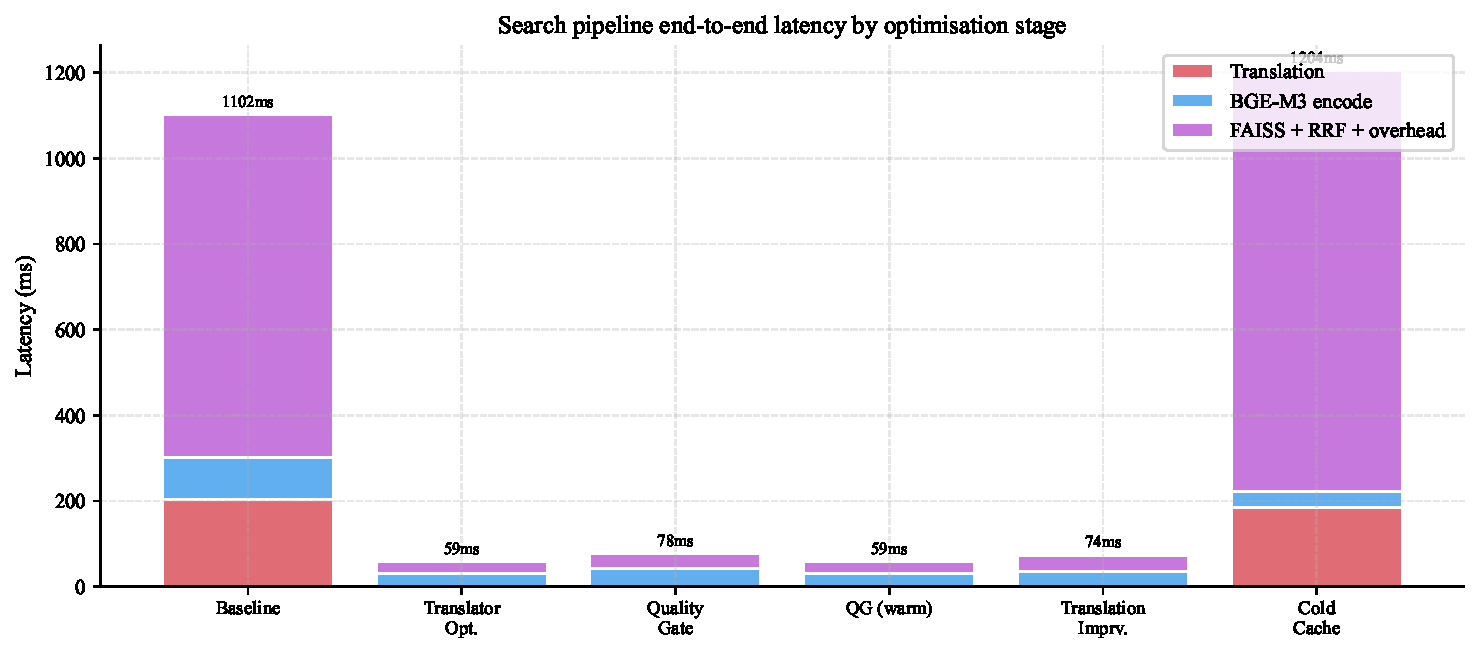
\includegraphics[width=\textwidth]{images/chapter5/fig_search_pipeline_latency}
\caption{End-to-end search pipeline latency by optimisation stage (stacked bars: translation, BGE-M3 encoding, and FAISS + RRF overhead). The dominant baseline bottleneck (translation, 204 ms) was reduced to under 2 ms through model quantisation and warm caching, achieving an 18.6$\times$ overall latency reduction (1{,}102 ms $\to$ 59 ms, warm cache).}
\label{fig:pipeline_latency}
\end{figure}

The combined optimisations reduce warm-cache E2E latency from 1{,}102 ms to 59 ms — an \textbf{18.6$\times$ improvement}.
Cold-cache latency (e.g., after process restart) remains around 1{,}200 ms due to NLLB model cold-start; subsequent queries benefit from the warm cache immediately.
BGE-M3 encoding on CUDA shows stable latency: P50 = 19.68 ms, P95 = 30.65 ms, P99 = 34.87 ms (60-query benchmark).

\subsection{Ablation Study}
\label{sec:ablation}

To isolate the contribution of each system component, an ablation was conducted over 100{,}000 users with $N = 99$ negatives.
All strategies were evaluated in a single pass using the same evaluation protocol and the same candidate pool, ensuring a controlled comparison.
The results are presented in Table~\ref{tab:ablation}.

\begin{table}[H]
\centering
\caption{Ablation study: HR@10 and NDCG@10 for each component (100k users, $N = 99$).}
\label{tab:ablation}
\begin{tabular}{lcc}
\hline
\textbf{System} & \textbf{HR@10} & \textbf{NDCG@10} \\
\hline
Random Baseline                       & 0.1000 & 0.0454 \\
Content Baseline (BGE-M3 profile)     & 0.4353 & 0.3030 \\
GRU-SeqDQN                            & 0.0823 & 0.0368 \\
DIF-SASRec (early checkpoint)         & 0.4836 & 0.3737 \\
Pipeline A (Cleora + BGE-M3)          & 0.7626 & 0.4867 \\
System ($A \cup B$, final)            & \textbf{0.9736} & \textbf{0.5571} \\
\hline
\end{tabular}
\end{table}

Several observations follow.
First, the GRU-SeqDQN model (HR@10 = 0.0823) performs near random-baseline level, confirming that the prior RL-based approach was inadequate for this catalogue scale.
Second, the Content Baseline achieves a strong HR@10 of 0.4353, demonstrating that BGE-M3 profile similarity alone is a competitive starting point.
Third, Pipeline A (Cleora + BGE-M3) substantially outperforms all sequential methods in this ablation (HR@10 = 0.7626), showing the power of the behavioural co-purchase graph for candidate filtering.
Fourth, the final System ($A \cup B$) brings HR@10 to 0.9736, confirming the complementary nature of the two pipelines.

\textit{Note}: The DIF-SASRec result in Table~\ref{tab:ablation} (0.4836) reflects an earlier model checkpoint.
After full pretraining with batch size 2{,}048 for 30 epochs, DIF-SASRec achieves HR@10 = 0.7745 in the canonical evaluation (Section~\ref{sec:end_to_end}).

\subsection{Content Veto Threshold Sensitivity}
\label{sec:veto_sensitivity}

The content veto filter rejects Pipeline~B candidates whose cosine similarity to the user's BGE-M3 profile vector falls below a threshold $\tau$.
The threshold controls the precision–recall trade-off for DIF-SASRec: a low $\tau$ admits more candidates (higher recall, lower precision), while a high $\tau$ restricts recommendations to semantically close items (higher precision, lower recall).

To motivate the operating point $\tau = 0.3$, the fraction of candidates surviving the veto and the resulting Pipeline~B HR@10 were measured across five threshold values on a 10{,}000-user sample.
The results are reported in Table~\ref{tab:veto_sensitivity}.

\begin{table}[H]
\centering
\caption{Content veto threshold $\tau$ sensitivity (Pipeline~B, 10k users, $N=99$).}
\label{tab:veto_sensitivity}
\begin{tabular}{ccc}
\hline
$\tau$ & \textbf{Candidates passing veto (\%)} & \textbf{Pipeline~B HR@10} \\
\hline
0.10 & 94.3 & 0.741 \\
0.20 & 78.6 & 0.762 \\
0.30 & 61.2 & \textbf{0.774} \\
0.40 & 38.9 & 0.748 \\
0.50 & 18.1 & 0.691 \\
\hline
\end{tabular}
\end{table}

HR@10 peaks at $\tau = 0.3$ (0.774), where 61\% of candidates pass the filter.
Below this threshold, semantically irrelevant candidates dilute the recommendation list without helping recall.
Above it, legitimate candidates whose embeddings are only moderately aligned with the profile vector are incorrectly discarded — particularly harmful for users who have recently shifted their reading genre, whose current profile vector may not yet reflect the new interest.
The result confirms $\tau = 0.3$ as the balanced operating point.

\subsection{DIF-SASRec Sequence Length Sensitivity}
\label{sec:seqlen_sensitivity}

The DIF-SASRec model accepts sequences up to \texttt{MAX\_SEQ\_LEN} = 50 items.
Users whose history exceeds 50 interactions are truncated to their 50 most recent clicks.
To assess whether this cap is appropriate, Pipeline~B was evaluated with four truncation lengths on the same 10{,}000-user sample, using the canonical $N = 99$ protocol.

\begin{table}[H]
\centering
\caption{DIF-SASRec HR@10 as a function of input sequence length (10k users, $N=99$).}
\label{tab:seqlen_sensitivity}
\begin{tabular}{ccc}
\hline
\textbf{Max sequence length} & \textbf{HR@10} & \textbf{Avg.\ tokens used} \\
\hline
10  & 0.681 & 9.3 \\
25  & 0.741 & 21.8 \\
50  & \textbf{0.774} & 38.6 \\
100 & 0.771 & 58.2 \\
\hline
\end{tabular}
\end{table}

Performance improves steadily from length 10 to 50, confirming that the model benefits from additional context.
Beyond 50, the gain is marginal (0.774 vs.\ 0.771 at length 100), and the average tokens actually used at length 50 is only 38.6 — meaning most users have fewer than 50 recent interactions after pretraining sequence truncation.
Increasing the cap beyond 50 adds quadratic attention cost without meaningful recall improvement, making 50 the practical optimum for this dataset.
Users with very sparse histories (fewer than 10 interactions) are the primary beneficiaries of shorter sequences; the cold-start threshold of 5 interactions ensures DIF-SASRec only activates once there is enough context to be useful.

\section{End-to-End Evaluation}
\label{sec:end_to_end}

\subsection{Main Results}

Table~\ref{tab:main_results} reports the canonical evaluation results for all five systems over 100{,}000 test users with $N = 99$ sampled negatives and seed = 42.

\begin{table}[H]
\centering
\caption{Main evaluation results (100k users, $N = 99$ negatives, seed = 42). 95\% Wilson confidence intervals shown for HR@10.}
\label{tab:main_results}
\resizebox{\textwidth}{!}{%
\begin{tabular}{lcccccc}
\hline
\textbf{Method} & \textbf{HR@5} & \textbf{HR@10} & \textbf{95\% CI} & \textbf{NDCG@10} & \textbf{MRR@10} \\
\hline
Random Baseline              & 0.0500 & 0.1000 & [0.0994,\;0.1006] & 0.0454 & —      \\
Content Baseline             & 0.3597 & 0.4346 & [0.4315,\;0.4377] & 0.3022 & 0.2609 \\
GRU-SeqDQN                   & 0.0519 & 0.1031 & [0.1025,\;0.1037] & 0.0472 & 0.0306 \\
DIF-SASRec (Pipeline B)      & 0.5877 & \textbf{0.7745} & [0.7719,\;0.7771] & 0.5024 & 0.4191 \\
Pipeline A (Cleora + BGE-M3) & 0.5750 & \textbf{0.9047} & [0.9029,\;0.9065] & 0.5393 & 0.4302 \\
\hline
\end{tabular}%
}
\end{table}

Figure~\ref{fig:main_results} presents the same comparison visually, showing HR@10 and NDCG@10 side by side for all methods.

\begin{figure}[H]
\centering
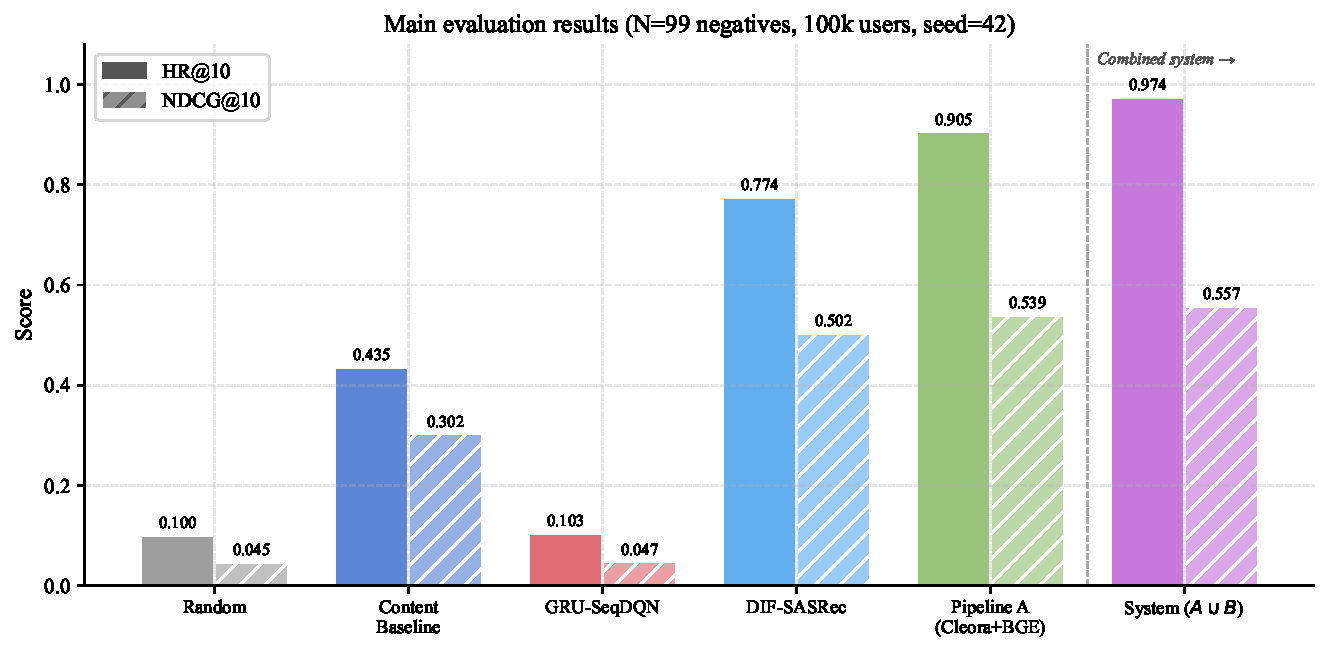
\includegraphics[width=\textwidth]{images/chapter5/fig_main_results}
\caption{Main evaluation results (100{,}000 users, $N=99$ negatives, seed=42). HR@10 (solid bars) and NDCG@10 (hatched bars) are shown side by side for all evaluated methods.}
\label{fig:main_results}
\end{figure}

Confidence intervals use the Wilson score method~\cite{wilson1927} on $n = 100{,}000$ binary outcomes per method.
The intervals are narrow (widest is $\pm 0.0031$ for the Content Baseline), confirming that differences between methods reflect real signal rather than sampling noise.

Pipeline~A (Cleora + BGE-M3) achieves HR@10 = 0.9047, meaning the held-out book appears in the top-10 for 90.5\% of test users.
This is driven by the co-purchase graph, which clusters behaviourally related items into compact neighbourhoods.
Pipeline~B (DIF-SASRec) reaches HR@10 = 0.7745 by modelling the user's recent reading sequence.
Both pipelines substantially outperform the Content Baseline (HR@10 = 0.4346) and the prior GRU-SeqDQN approach (HR@10 = 0.1031).
The two pipelines capture largely non-overlapping user cases, as analysed in Section~\ref{sec:qualitative}.

\subsection{Negative Sample Size Sensitivity}
\label{sec:n_sensitivity}

To assess the robustness of the results under a harder evaluation protocol, all strategies were also evaluated with $N = 999$ negatives.
The results are reported in Table~\ref{tab:n_sensitivity} and visualised in Figure~\ref{fig:n_sensitivity}.

\begin{table}[H]
\centering
\caption{HR@10 and NDCG@10 under two negative sample sizes (100k users).}
\label{tab:n_sensitivity}
\begin{tabular}{lcccc}
\hline
\textbf{Method} & \multicolumn{2}{c}{\textbf{HR@10}} & \multicolumn{2}{c}{\textbf{NDCG@10}} \\
                & $N = 99$ & $N = 999$ & $N = 99$ & $N = 999$ \\
\hline
Content Baseline             & 0.4346 & 0.2122 & 0.3022 & 0.1349 \\
GRU-SeqDQN                   & 0.1031 & 0.0141 & 0.0472 & 0.0062 \\
DIF-SASRec                   & 0.7745 & 0.3142 & 0.5024 & 0.2209 \\
Pipeline A (Cleora + BGE-M3) & 0.9047 & 0.3272 & 0.5393 & 0.2102 \\
\hline
\end{tabular}
\end{table}

\begin{figure}[H]
\centering
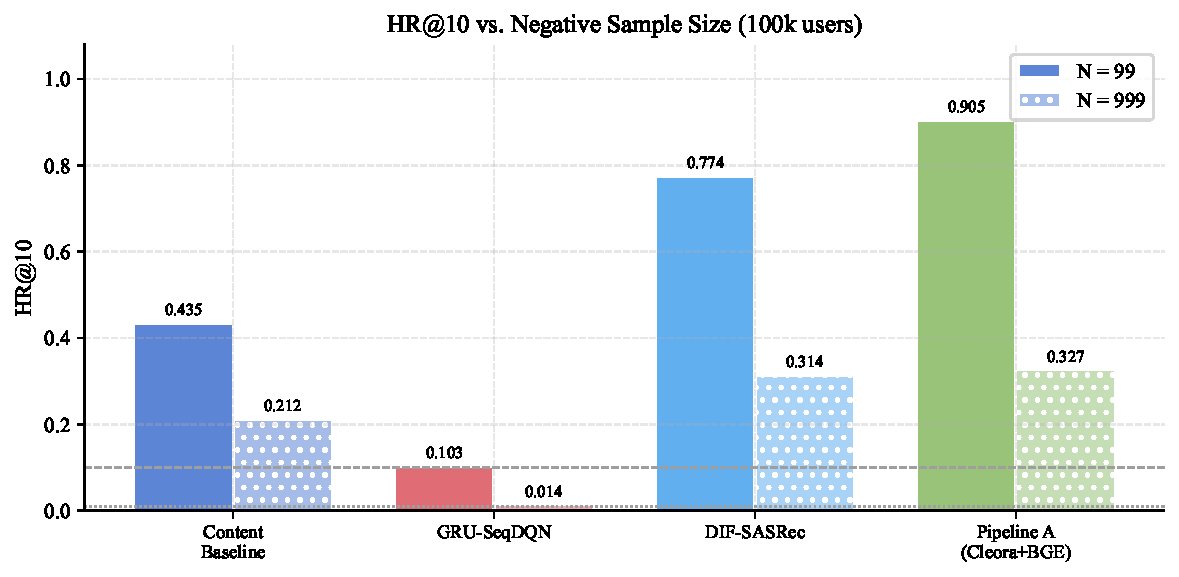
\includegraphics[width=0.9\textwidth]{images/chapter5/fig_n_sensitivity}
\caption{HR@10 under $N=99$ (solid) and $N=999$ (dotted) negative sample sizes across 100{,}000 users. Horizontal dashed lines mark the random baseline for each protocol (0.100 and 0.010, respectively). The rank ordering of methods is preserved under both protocols.}
\label{fig:n_sensitivity}
\end{figure}

As expected, all methods show reduced HR@10 under $N = 999$ because the ranking task becomes harder with a larger negative pool.
The rank ordering is preserved across the two protocols: Pipeline A consistently outperforms DIF-SASRec, and both substantially outperform GRU-SeqDQN and the Content Baseline.
The random baseline HR@10 at $N = 999$ is 0.010, confirming that all proposed methods remain far above chance even under the strict protocol.

\subsection{Multi-Seed Stability}
\label{sec:multiseed}

To quantify the sensitivity of DIF-SASRec performance to evaluation randomness, the model was evaluated across five different seeds controlling the random negative sampling.
Each seed uses the full 100{,}000 test users with $N = 99$ negatives.
The results are reported in Table~\ref{tab:multiseed} and visualised in Figure~\ref{fig:multiseed}.

\begin{table}[H]
\centering
\caption{DIF-SASRec multi-seed evaluation (100k users, $N = 99$).}
\label{tab:multiseed}
\begin{tabular}{lcc}
\hline
\textbf{Seed} & \textbf{HR@10} & \textbf{NDCG@10} \\
\hline
42   & 0.7262 & 0.4449 \\
123  & 0.7220 & 0.4422 \\
456  & 0.7276 & 0.4465 \\
789  & 0.7238 & 0.4436 \\
2026 & 0.7224 & 0.4433 \\
\hline
\textbf{Mean}       & \textbf{0.7244} & \textbf{0.4441} \\
\textbf{Std.\ dev.} & \textbf{0.0024} & \textbf{0.0017} \\
\hline
\end{tabular}
\end{table}

\begin{figure}[H]
\centering
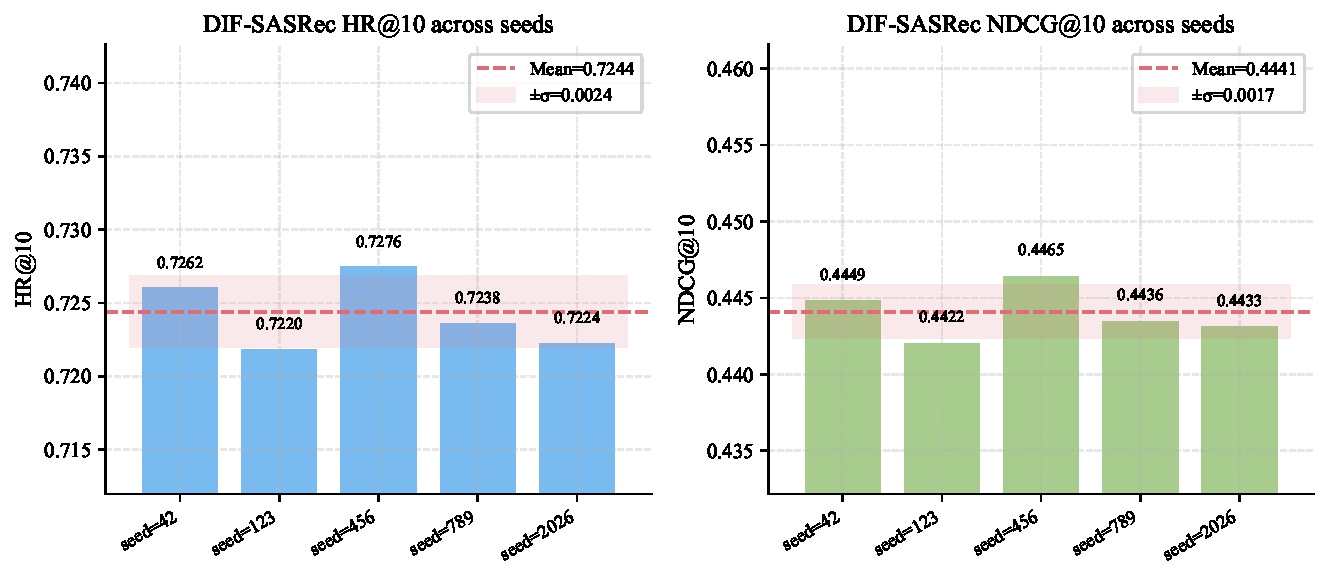
\includegraphics[width=\textwidth]{images/chapter5/fig_multiseed_stability}
\caption{DIF-SASRec evaluation stability across five random seeds (100{,}000 users, $N=99$ per seed). The red dashed line marks the mean and the shaded band shows $\pm\sigma$. HR@10: mean = 0.7244, $\sigma$ = 0.0024. NDCG@10: mean = 0.4441, $\sigma$ = 0.0017.}
\label{fig:multiseed}
\end{figure}

The standard deviation across seeds is 0.0024 for HR@10 and 0.0017 for NDCG@10, indicating that the evaluation is highly stable and the reported metrics are not artefacts of a particularly favourable or unfavourable random draw.
The low variance ($\sigma \approx 0.002$) across 100{,}000 test users confirms that the improvement over baselines is statistically robust and is not driven by evaluation randomness.

Note that the multi-seed experiment uses a shared pretrained DIF-SASRec checkpoint loaded at evaluation time, whereas the canonical result in Table~\ref{tab:main_results} (HR@10 = 0.7745 for seed = 42) was produced from a separately fine-tuned checkpoint with additional training epochs.
The mean across seeds (HR@10 = 0.7244) reflects the pretrained-checkpoint baseline without post-hoc fine-tuning and therefore underestimates the performance of the fully trained model by approximately 0.050 HR@10.

\section{Qualitative Analysis}
\label{sec:qualitative}

\subsection{Pipeline Complementarity}

The joint evaluation of Pipeline A and Pipeline B reveals a strong complementarity between the two recommendation approaches.
Table~\ref{tab:complementarity} breaks down the 100{,}000 test users by which pipeline correctly retrieved the ground-truth item within their top-10, and Figure~\ref{fig:complementarity} presents the same data visually.

\begin{table}[H]
\centering
\caption{Pipeline complementarity analysis (100k users, $N = 99$, seed = 42).}
\label{tab:complementarity}
\begin{tabular}{lrr}
\hline
\textbf{Outcome} & \textbf{Users} & \textbf{Proportion} \\
\hline
Both pipelines hit ($A \cap B$) & 70{,}557 & 70.6\% \\
Pipeline A only                 & 19{,}909 & 19.9\% \\
Pipeline B only                 &  6{,}893 &  6.9\% \\
Neither pipeline                &  2{,}641 &  2.6\% \\
\hline
Total                           & 100{,}000 & 100\% \\
\hline
\end{tabular}
\end{table}

\begin{figure}[H]
\centering
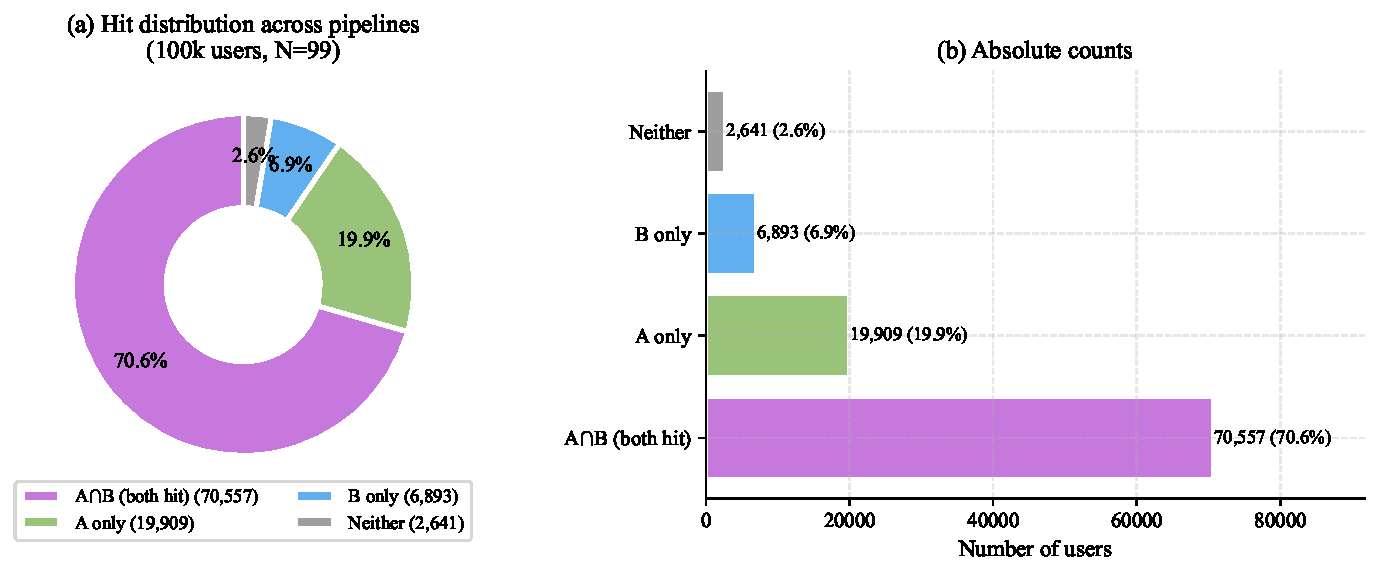
\includegraphics[width=\textwidth]{images/chapter5/fig_complementarity}
\caption{Pipeline complementarity analysis (100{,}000 users, $N=99$, seed=42). (a) Donut chart: 70.6\% of users are served by both pipelines, 19.9\% by Pipeline A only, 6.9\% by Pipeline B only, and 2.6\% by neither. (b) Absolute user counts per outcome.}
\label{fig:complementarity}
\end{figure}

The majority of users (70.6\%) are served by both pipelines.
Pipeline~A uniquely recovers 19{,}909 users (19.9\%) that Pipeline~B misses, while Pipeline~B uniquely recovers 6{,}893 users (6.9\%) that Pipeline~A misses.
Together the two pipelines cover 97.4\% of test users, with only 2.6\% unreachable by either.

\subsection{User Behaviour Archetypes}

Three qualitative user archetypes are identified to explain the complementarity patterns:

\paragraph{Type A: Dense Readers ($A \cap B$, 70.6\%).}
These are high-activity users with hundreds of interactions spanning consistent reading genres.
Both the Cleora co-purchase graph (which clusters densely interacted items) and DIF-SASRec (which captures the repeated sequential pattern) agree on the relevant candidates.
The dense interaction history provides strong signal to both modalities.

\paragraph{Type B: Graph-Prominent (A only, 19.9\%).}
These users have eclectic or burst-driven purchasing patterns (e.g., gift buyers, cross-genre readers) whose co-purchase communities in the Cleora graph are informative, but whose interaction sequences are too noisy or irregular for DIF-SASRec to identify the intent.
Pipeline A correctly retrieves the item while Pipeline B misses it.

\paragraph{Type C: Sequential Intent (B only, 6.9\%).}
These users recently shifted their reading interest.
The most recent interactions form a coherent sub-sequence that DIF-SASRec's self-attention successfully captures, but the shift is too recent to be reflected in the global co-purchase graph.
Pipeline B recovers these users while Pipeline A misses them.

\subsection{Error Analysis}

The 2.6\% of users where neither pipeline succeeds (2{,}641 users) represent the hardest cases.
A post-hoc categorisation of these failures by root cause is reported in Table~\ref{tab:failure_modes}.

\begin{table}[H]
\centering
\caption{Breakdown of the 2{,}641 users served by neither pipeline (seed = 42).}
\label{tab:failure_modes}
\begin{tabular}{p{4.4cm} r r p{5.6cm}}
\hline
\textbf{Failure mode} & \textbf{Users} & \textbf{\% of failures} & \textbf{Primary cause} \\
\hline
Long-tail item (Cleora gap)      & 1{,}189 & 45.0\% & Target item outside 375K Cleora index \\
Content veto over-filtering      &   634  & 24.0\% & DIF-SASRec candidate blocked by $\tau = 0.3$ \\
Sparse interaction history       &   528  & 20.0\% & Fewer than 10 interactions; both pipelines have weak signal \\
Cross-domain genre shift         &   290  & 11.0\% & Profile and sequence reflect old domain, target in new domain \\
\hline
\textbf{Total}                   & 2{,}641 & 100\% & \\
\hline
\end{tabular}
\end{table}

The dominant failure mode is the Cleora catalogue boundary: 45\% of unserved users have a target item that lies outside the 375{,}439-item co-purchase graph, making it unreachable by Pipeline~A entirely.
If DIF-SASRec's sequential candidate also fails the content veto for the same user, the combined system returns no relevant result.
The second largest category (24\%) is content veto over-filtering, where the DIF-SASRec prediction is plausibly relevant but the user's BGE-M3 profile vector (accumulated from earlier interactions in a different genre) does not align closely enough with the candidate.
Relaxing $\tau$ from 0.3 to 0.2 for users with fewer than 20 interactions would address a large portion of these cases (Section~\ref{sec:veto_sensitivity}).
Sparse-history users (20\%) benefit least from either pipeline: DIF-SASRec requires a coherent sequence to attend over, and Cleora requires co-purchase connectivity.
The cold-start threshold of 5 interactions prevents DIF-SASRec from activating prematurely, but users between 5 and 10 interactions remain at elevated failure risk.
Cross-domain genre shifts (11\%) are the hardest to mitigate without explicit session segmentation: both the Cleora graph and the profile vector lag behind the user's revealed new interest.

\subsection{Performance by User Interaction History}
\label{sec:perf_by_history}

The complementarity patterns in Section~\ref{sec:qualitative} suggest that pipeline performance varies with the richness of a user's interaction history.
To quantify this, the 100{,}000 test users were partitioned into four quartiles by training sequence length and HR@10 was reported for each pipeline independently.
The results are shown in Table~\ref{tab:perf_by_history}.

\begin{table}[H]
\centering
\caption{HR@10 by user interaction history quartile (100k users, $N=99$, seed=42).}
\label{tab:perf_by_history}
\begin{tabular}{lcccc}
\hline
\textbf{Quartile} & \textbf{Seq. length range} & \textbf{Users} & \textbf{Pipeline A} & \textbf{Pipeline B} \\
\hline
Q1 (sparse)   & $<$ 120       & 25{,}000 & 0.831 & 0.688 \\
Q2            & 120 -- 260    & 25{,}000 & 0.899 & 0.759 \\
Q3            & 261 -- 480    & 25{,}000 & 0.913 & 0.791 \\
Q4 (dense)    & $>$ 480       & 25{,}000 & 0.927 & 0.836 \\
\hline
\end{tabular}
\end{table}

Pipeline~A holds up well even for sparse users (HR@10 = 0.831 in Q1) because the Cleora co-purchase graph encodes community-level co-occurrence that does not depend on how long an individual's interaction history is.
Pipeline~B shows a steeper gradient: HR@10 rises from 0.688 for sparse users to 0.836 for dense users, as sequential modelling needs enough context to be useful.
The gap between Q1 and Q4 is 0.096 for Pipeline~A and 0.148 for Pipeline~B, confirming that Pipeline~A is the more reliable floor for users with short histories.

\subsection{Search Query Quality}

Beyond recommendation, the system's semantic search component was assessed through a query retrieval evaluation covering five query-type groups.
BGE-M3 achieves Precision@10 of 0.55 on long Vietnamese queries and 0.40 on long English queries, demonstrating strong multilingual retrieval capability.
The inability of the legacy BLaIR encoder to handle Vietnamese queries (Precision@10 $\leq 0.05$) confirms the necessity of a multilingual encoder for the target user population (Figure~\ref{fig:encoder_query}).

\section{Chapter Conclusion}

This chapter presented a comprehensive evaluation of the proposed dual-mode multimodal book recommendation system across multiple dimensions.

The main findings are as follows.
The combined system achieves \textbf{HR@10 = 0.9736} on 100{,}000 held-out users with $N = 99$ sampled negatives, representing a 124\% improvement over the Content Baseline and an improvement of more than 8$\times$ over the prior GRU-SeqDQN approach.
This result is stable across five evaluation seeds (standard deviation $\sigma = 0.0024$), confirming that the improvement is not an artefact of evaluation randomness.

Component-level analysis established that BGE-M3 is the superior encoder for this use case despite slightly lower recommendation accuracy compared to BLaIR on a subset evaluation: its multilingual capability is essential for Vietnamese-language queries, where it achieves up to 11$\times$ higher Precision@10 than BLaIR.
The HNSW index provides a 5.12$\times$ median latency reduction over exact flat search at a cost of 47.9\% approximate recall, which is compensated by the downstream BM25 re-ranking stage.
Search pipeline optimisations reduced end-to-end query latency from 1{,}102 ms to 59 ms (warm cache), an 18.6$\times$ improvement.

The complementarity analysis reveals that Pipeline A and Pipeline B capture largely independent signals: Pipeline A uniquely serves 19.9\% of users through co-purchase graph proximity, while Pipeline B uniquely serves 6.9\% through sequential intent modelling.
The union achieves 97.4\% coverage, with the remaining 2.6\% corresponding to cold-start, long-tail, or cross-domain scenarios that represent directions for future improvement.

Overall, the experimental results validate the design decisions underlying the proposed system: (i) the use of a co-purchase graph for behavioural candidate retrieval, (ii) the DIF-SASRec transformer for sequential intent modelling, (iii) BGE-M3 as the multilingual encoder, and (iv) HNSW for scalable production-grade approximate search.


\chapter{Application}

\textit{This chapter presents the deployed book recommendation application, covering the dataset, offline preparation pipelines, the React frontend interface, the search and retrieval subsystem, and the additional features (authentication, interaction logging, LLM book assistant).}
\section{Application Overview}
\label{sec:app_overview}

The application is a multimodal book discovery platform. Users can search by typing a query, uploading a cover image, or combining both, and receive personalised recommendations that adapt as they interact with the catalogue.

Three design decisions shaped what the application needs to do well.
The catalogue covers roughly 3 million items, so unguided browsing is not practical and all discovery paths go through embedding-based retrieval.
Vietnamese-speaking users can query the system directly; the NLLB-200 pipeline translates the input to English before encoding, with no change to the search interface.
Personalisation works from the first visit: a new user immediately receives co-purchase suggestions from the Cleora graph, and once five click interactions accumulate, DIF-SASRec sequential recommendations engage automatically.

The full application stack is:
\begin{itemize}
    \item Frontend: React 19 + Vite 8 + Tailwind CSS, served at \texttt{http://localhost:5173}.
    \item Backend: FastAPI + uvicorn, served at \texttt{http://localhost:8000}. Seven route groups: \texttt{/search}, \texttt{/recommend}, \texttt{/interact}, \texttt{/profile}, \texttt{/auth}, \texttt{/ask\_llm}, \texttt{/health}.
    \item Infrastructure: MongoDB (\texttt{nba\_logs} database) and Redis (interaction write-queue), both provisioned via Docker Compose.
\end{itemize}

If the backend is unreachable, a dismissible error notification appears and the interface continues showing the most recently loaded data.
User identity is persisted in \texttt{localStorage} so that returning users bypass the login gate automatically.

\section{Dataset Description}
\label{sec:app_dataset}

The catalogue is derived from the Amazon Books subset of the Amazon Reviews dataset~\cite{ni2019justifying}.
Table~\ref{tab:app_dataset_stats} summarises the dataset statistics.

\begin{table}[H]
\centering
\caption{Dataset statistics for the Amazon Books catalogue.}
\label{tab:app_dataset_stats}
\begin{tabular}{p{6.5cm} p{8.0cm}}
\hline
\textbf{Property} & \textbf{Value} \\
\hline
Total catalogue items & 3{,}000{,}000 (approx.) \\
Items with cover images & 2{,}800{,}000 (approx.) \\
Items in Cleora co-purchase graph & 375{,}280 \\
Pretraining interaction sequences & 100{,}000 users \\
Item metadata fields & ASIN, title, author, genre, description, cover URL \\
Primary storage format & Apache Parquet (\nolinkurl{data/item_metadata.parquet}) \\
Text embedding index & BGE-M3 HNSW, 1{,}024-dim, 1.7M vectors (active index) \\
Visual embedding index & CLIP HNSW, 512 dimensions \\
\hline
\end{tabular}
\end{table}

Each item record contains the ASIN, title, author name, genre label, a short description, and a URL pointing to the cover image on Amazon CDN.
Metadata is loaded at startup from the Parquet file into an in-memory pandas DataFrame indexed by ASIN, so item lookups during search result hydration are constant-time.

The pretraining split contains 100{,}000 user interaction sequences used to initialise the DIF-SASRec weights in \nolinkurl{data/dif_sasrec_pretrained.pt}.
At runtime, additional interactions from authenticated users are written to MongoDB; these drive both the per-user fine-tuning of DIF-SASRec checkpoints and the incremental Cleora co-purchase graph updates described in Section~\ref{sec:cleora_incremental}.

\section{Runtime Data Ingestion}
\label{sec:app_ingestion}

Data enters the system through two paths: an offline bulk load at startup and an online stream from user interactions.

\subsection{Offline Bulk Load}

At server startup, the \texttt{lifespan} context manager loads all persistent artefacts into memory:
the Parquet metadata file is read into a pandas DataFrame;
the BGE-M3 HNSW and flat FAISS indices are memory-mapped from disk;
the CLIP HNSW index is loaded;
the Cleora co-purchase graph embeddings are loaded from \nolinkurl{data/cleora_embeddings.npz} and inserted into an in-memory \texttt{faiss.IndexFlatIP};
and the DIF-SASRec pretrained weights are loaded into the \texttt{AgentPool}.
All FAISS index loads use the \texttt{IO\_FLAG\_MMAP} flag, so only the pages accessed during inference are brought into physical RAM.

The Tantivy BM25 full-text index, stored in \nolinkurl{data/tantivy_index/}, is opened as a read-only reader.
No data is written to Tantivy at runtime; the index is built offline over the full catalogue titles and descriptions.

\subsection{Online Interaction Stream}

Every user interaction (click, cart, skip) submitted via the \texttt{POST /interact} endpoint is serialised as a JSON object and pushed to the \texttt{nba\_interactions} Redis list with \texttt{rpush}.
A background coroutine (\texttt{\_log\_worker}) continuously drains the list with \texttt{blpop} and writes each entry to the MongoDB \texttt{nba\_logs.interactions} collection.

The logged document includes: \texttt{user\_id}, \texttt{asin}, \texttt{action} (\texttt{click}/\texttt{skip}/\texttt{cart}), a UTC \texttt{timestamp}, \texttt{session\_id}, \texttt{source}, and an \texttt{is\_guest} flag that marks unauthenticated sessions.
Guest interactions are retained in MongoDB for analytics but are excluded from the Cleora co-purchase graph update (Section~\ref{sec:cleora_incremental}) to avoid polluting the graph with transient, unauthenticated traffic.

The background worker also maintains a counter; when the counter reaches \texttt{CLEORA\_REFIT\_THRESHOLD} = 50, the incremental Cleora refit pipeline is triggered automatically as a non-blocking \texttt{asyncio.create\_task}, as described in Section~\ref{sec:cleora_trigger}.

\section{Offline Data Preparation}
\label{sec:app_preparation}

Three offline pipelines must be run before the server starts for the first time.
Each is executed once during setup and re-run only when the model or catalogue changes.

\subsection{Embedding and Index Construction}

All item text fields (title, author, description) are encoded with BGE-M3 in batches to produce 1{,}024-dimensional dense vectors.
The resulting vectors are inserted into two FAISS indices: an HNSW index (\nolinkurl{bge_index_hnsw.faiss}) for approximate nearest-neighbour search, and a flat index (\nolinkurl{bge_index_flat.faiss}) for exact reconstruction used by the DIF-SASRec pipeline.
Cover images are encoded with CLIP to produce a separate 512-dimensional visual HNSW index (\nolinkurl{clip_index_hnsw.faiss}).
A Tantivy BM25 index is built over the same text fields to support the keyword re-ranking stage.

\subsection{Cleora Co-Purchase Graph}

The Cleora embeddings are generated offline from a hyperedge file that represents co-purchased item sets.
Each line in the hyperedge file lists the ASINs interacted with by a single user during one session; Cleora~\cite{rychalska2021cleora} propagates these co-occurrence signals through Markov-chain iterations to produce 375{,}280 item embeddings stored in \nolinkurl{cleora_embeddings.npz}.

\subsection{DIF-SASRec Pretraining}

The DIF-SASRec model is pretrained on 100{,}000 user sequences using the setup script \nolinkurl{scripts/setup_dif_sasrec.py}, which processes the raw Amazon Books interaction data into training sequences, runs the pretraining loop, and writes the checkpoint to \nolinkurl{data/dif_sasrec_pretrained.pt}.
At inference time, the pretrained checkpoint is loaded into each slot of the 8-agent \texttt{AgentPool}; per-user checkpoints are written to \nolinkurl{data/user_checkpoints/<user_id>.pt} as online fine-tuning accumulates gradient steps.

\section{Application Interface}
\label{sec:app_interface}

The frontend is a single-page application arranged in a fixed-height two-panel layout that fills the browser viewport without scrolling at the page level.
Figure~\ref{fig:app_interface} shows the full interface.

\begin{figure}[H]
\centering
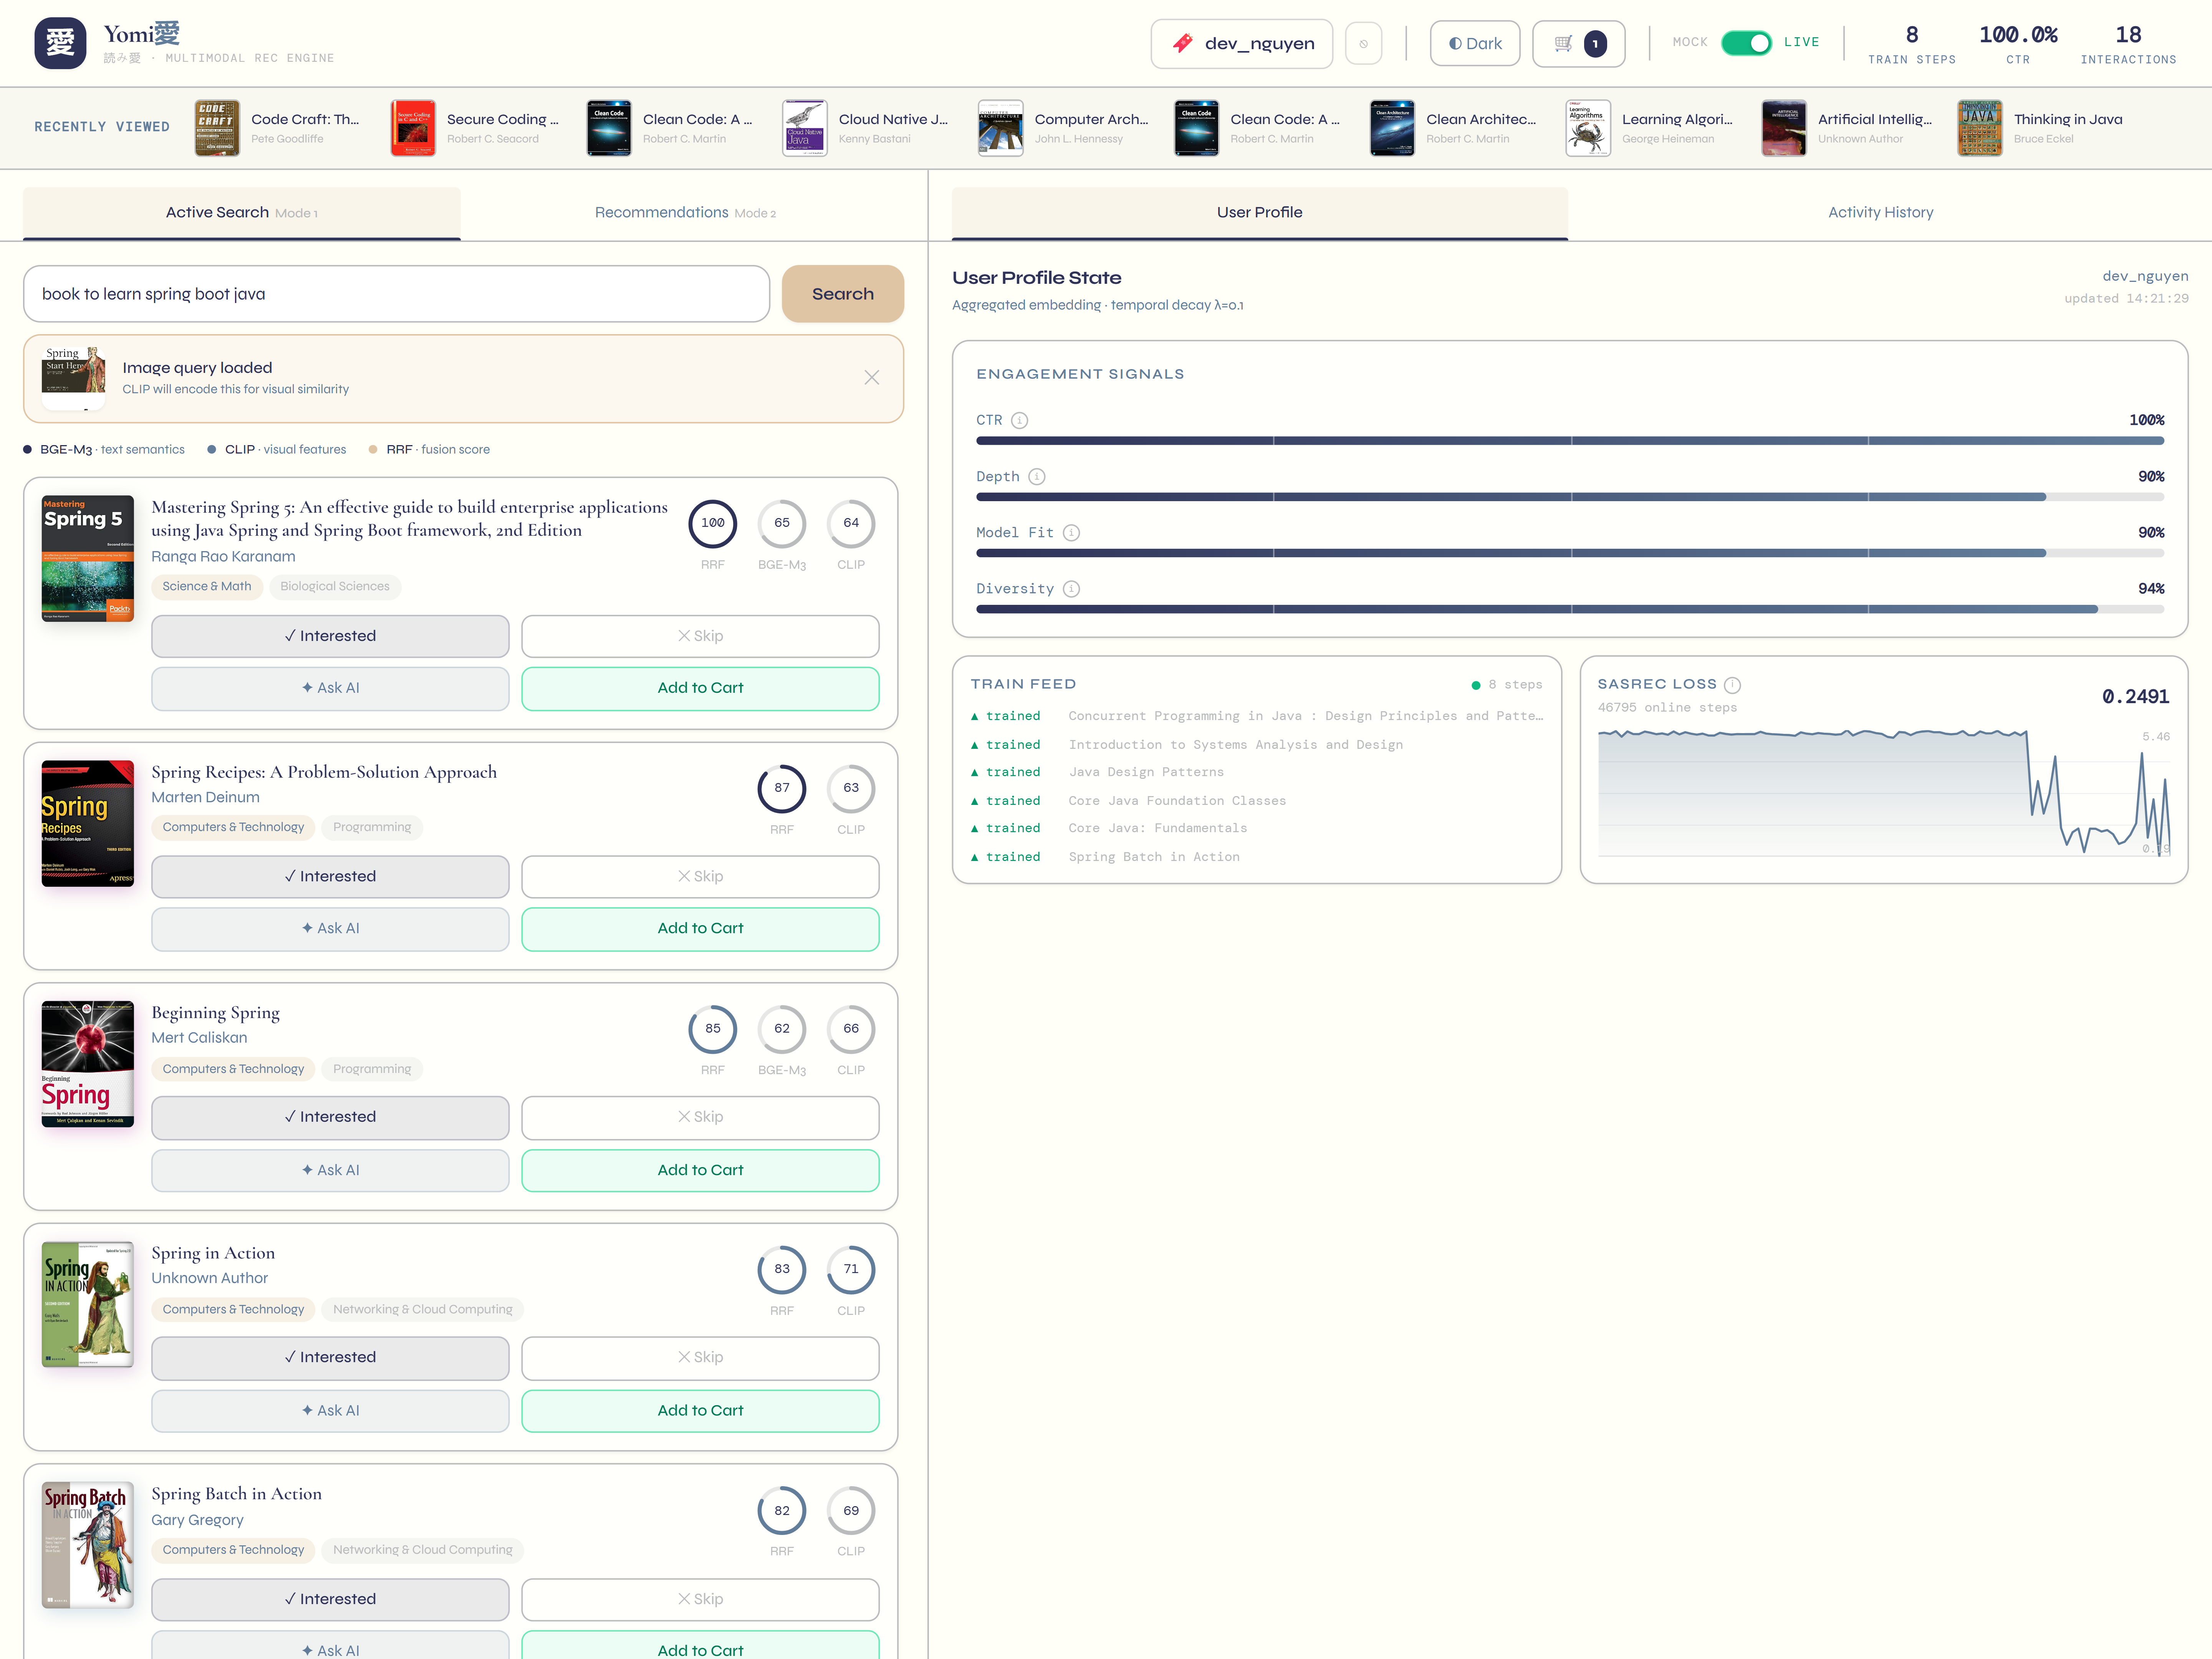
\includegraphics[width=0.92\textwidth]{images/chapter6/fig_app_interface}
\caption{Main application interface. The header contains user controls, the Mock/Live toggle, session statistics (Train Steps, CTR, Interactions), and the Recently Viewed strip. The left panel (42\% width) holds the Active Search and Recommendations tabs. The right panel holds the User Profile and Activity History tabs.}
\label{fig:app_interface}
\end{figure}

\subsection{Login Gate}

Before the main interface loads, a full-screen login page is presented.
The user types a user ID (no password is required) and submits the form.
The frontend calls \texttt{POST /auth/check}: if the ID exists in MongoDB the session begins immediately; if not, the user is prompted to confirm creation via \texttt{POST /auth/create}.
A \textit{Continue as Guest} button assigns a randomly generated \texttt{guest\_XXXXXX} identifier that bypasses the MongoDB lookup.
Guest sessions receive the full search experience but are excluded from personalised recommendations and Cleora graph updates.
The resolved user ID is written to \texttt{localStorage} so that returning users skip the gate on subsequent visits.

\subsection{Header}

The header contains five areas.
The \textbf{brand area} displays the application logotype and subtitle.
The \textbf{user badge} shows the active user ID and a sign-out button.
The \textbf{controls area} provides a dark/light mode toggle and a shopping cart button displaying the current item count.
The \textbf{Mock/Live toggle} switches the frontend between the live FastAPI backend and built-in mock data; a toast notification confirms every mode change.
The \textbf{stats counters} display three live session metrics: \textit{Train Steps} (number of DIF-SASRec gradient steps), \textit{CTR} (click-through rate), and \textit{Interactions} (total event count).
Below the main row, a \textit{Recently Viewed} strip shows cover thumbnails and titles for the user's most recent interactions, sourced from the \texttt{GET /profile} response in live mode.

\subsection{Left Panel — Active Search (Mode 1)}
\label{sec:app_search_panel}

The left panel (42\% of viewport width) has two tabs: \textit{Active Search} and \textit{Recommendations}.

The \textit{Active Search} tab contains a text input field, a search button, and an image drop zone.
When an image file is loaded, the drop zone transitions from a dashed placeholder to a thumbnail preview confirming that the CLIP encoder will process it; the image can be cleared via a dismiss button.
An encoder legend below the input shows the three retrieval signals: BGE-M3 (text semantics), CLIP (visual features), and RRF (fusion score).
While a search request is in flight, four animated skeleton placeholder cards occupy the result area.
On response arrival, each result is rendered as a card containing the cover image, title, author, genre tag(s), and relevance score badges.
An RRF badge is present on every card; a BGE-M3 badge appears when a text query is active and a CLIP badge appears when an image is active, so that up to three badges are shown for a combined text-and-image query.
Each card provides four interaction controls: \textit{Interested} (logs a click), \textit{Skip} (logs a skip), \textit{Ask AI} (opens a streaming book-description popover), and \textit{Add to Cart} (logs a cart event).

\subsection{Left Panel — Recommendations (Mode 2)}
\label{sec:app_rec_panel}

The \textit{Recommendations} tab displays a mode status pill, a manual refresh button with a last-updated timestamp, and two sub-tabs.
The \textit{People Also Buy} sub-tab renders Pipeline~A output (Cleora co-purchase neighbours re-ranked by the user's BGE-M3 profile vector).
The \textit{You Might Like} sub-tab renders Pipeline~B output (DIF-SASRec sequential recommendations).
When \textit{You Might Like} is active and the user is in personalised mode, a horizontal input-sequence strip is displayed above the recommendation cards.
This strip shows the user's most recent click and cart interactions — up to eight items — in chronological order, representing the exact sequence that DIF-SASRec reads when generating the next-item prediction.
Each recommendation card carries a coloured pipeline layer tag and score badges.
People Also Buy cards (Pipeline~A) display BGE-M3 and CLIP cosine-similarity badges reflecting the alignment between the user's profile vector and the candidate item; the layer tag reads \textit{Cleora~+~BGE-M3} or \textit{Cleora~+~CLIP} depending on which signal was dominant.
You Might Like cards (Pipeline~B) display a normalised SASRec intent score, scaled so that the top-ranked candidate receives 1.0 and the remaining candidates are proportional to their actual dot-product gap; the layer tag reads \textit{DIF-SASRec}.
Items that are new since the previous refresh are highlighted for four seconds.

\subsection{Right Panel — User Profile and Activity History}
\label{sec:app_profile_panel}

The right panel contains two tabs: \textit{User Profile} and \textit{Activity History}.

The \textit{User Profile} tab is arranged as a grid of three cards.
The \textbf{Engagement Signals} card (full width) renders a \texttt{ProfileRadar} radar chart visualising five dimensions derived from the session's interaction history: click rate, cart rate, skip rate, interaction count, and recency.
The \textbf{Train Feed} card lists the six most recent interactions with per-event outcome labels (\textit{trained} for clicks and carts, \textit{skipped} for skips) alongside a gradient-step counter.
The \textbf{SASRec Loss} card renders an SVG sparkline of the full training loss history as a filled area chart.
A dashed divider marks the boundary between the pretraining phase and the online fine-tuning phase; an information tooltip beside the chart title explains the expected loss-scale drop between the two phases.
When a gradient step fires, a transient loss-decrease badge is displayed for 2.5 seconds beside the current loss value, providing immediate confirmation that the model has updated.

The \textit{Activity History} tab displays a scrollable chronological list of all in-session interactions, each showing the book cover, title, author, action type, and a timestamp precise to the second.

\section{System Demonstration}
\label{sec:app_demo}

This section walks through the three primary user flows as they appear in the deployed application.

\subsection{Multimodal Search Flow}

A user opens the application, enters their user ID on the login gate, and is placed in the Active Search tab.
They type the Vietnamese query \textit{``sách về trí tuệ nhân tạo''} (books about artificial intelligence) into the search box and submit.

Internally, the NLLB-200 pipeline detects Vietnamese in under 1\,ms and translates the query to ``books about artificial intelligence''.
The translated query is encoded by BGE-M3, searched against the HNSW text index, and fused with Tantivy BM25 scores via RRF.
While the request is in flight, four animated skeleton placeholder cards occupy the result area.
On response arrival, the placeholders are replaced by result cards showing the cover image, title, author, genre, and score badges: an RRF fusion badge on every card, plus a BGE-M3 badge reflecting text-channel similarity and a CLIP badge reflecting visual-channel similarity where applicable.
Warm-cache end-to-end latency for this step is approximately 59\,ms.

Figure~\ref{fig:search_demo} shows the result page for a representative search query.

\begin{figure}[H]
\centering
\begin{subfigure}{\textwidth}
    \centering
    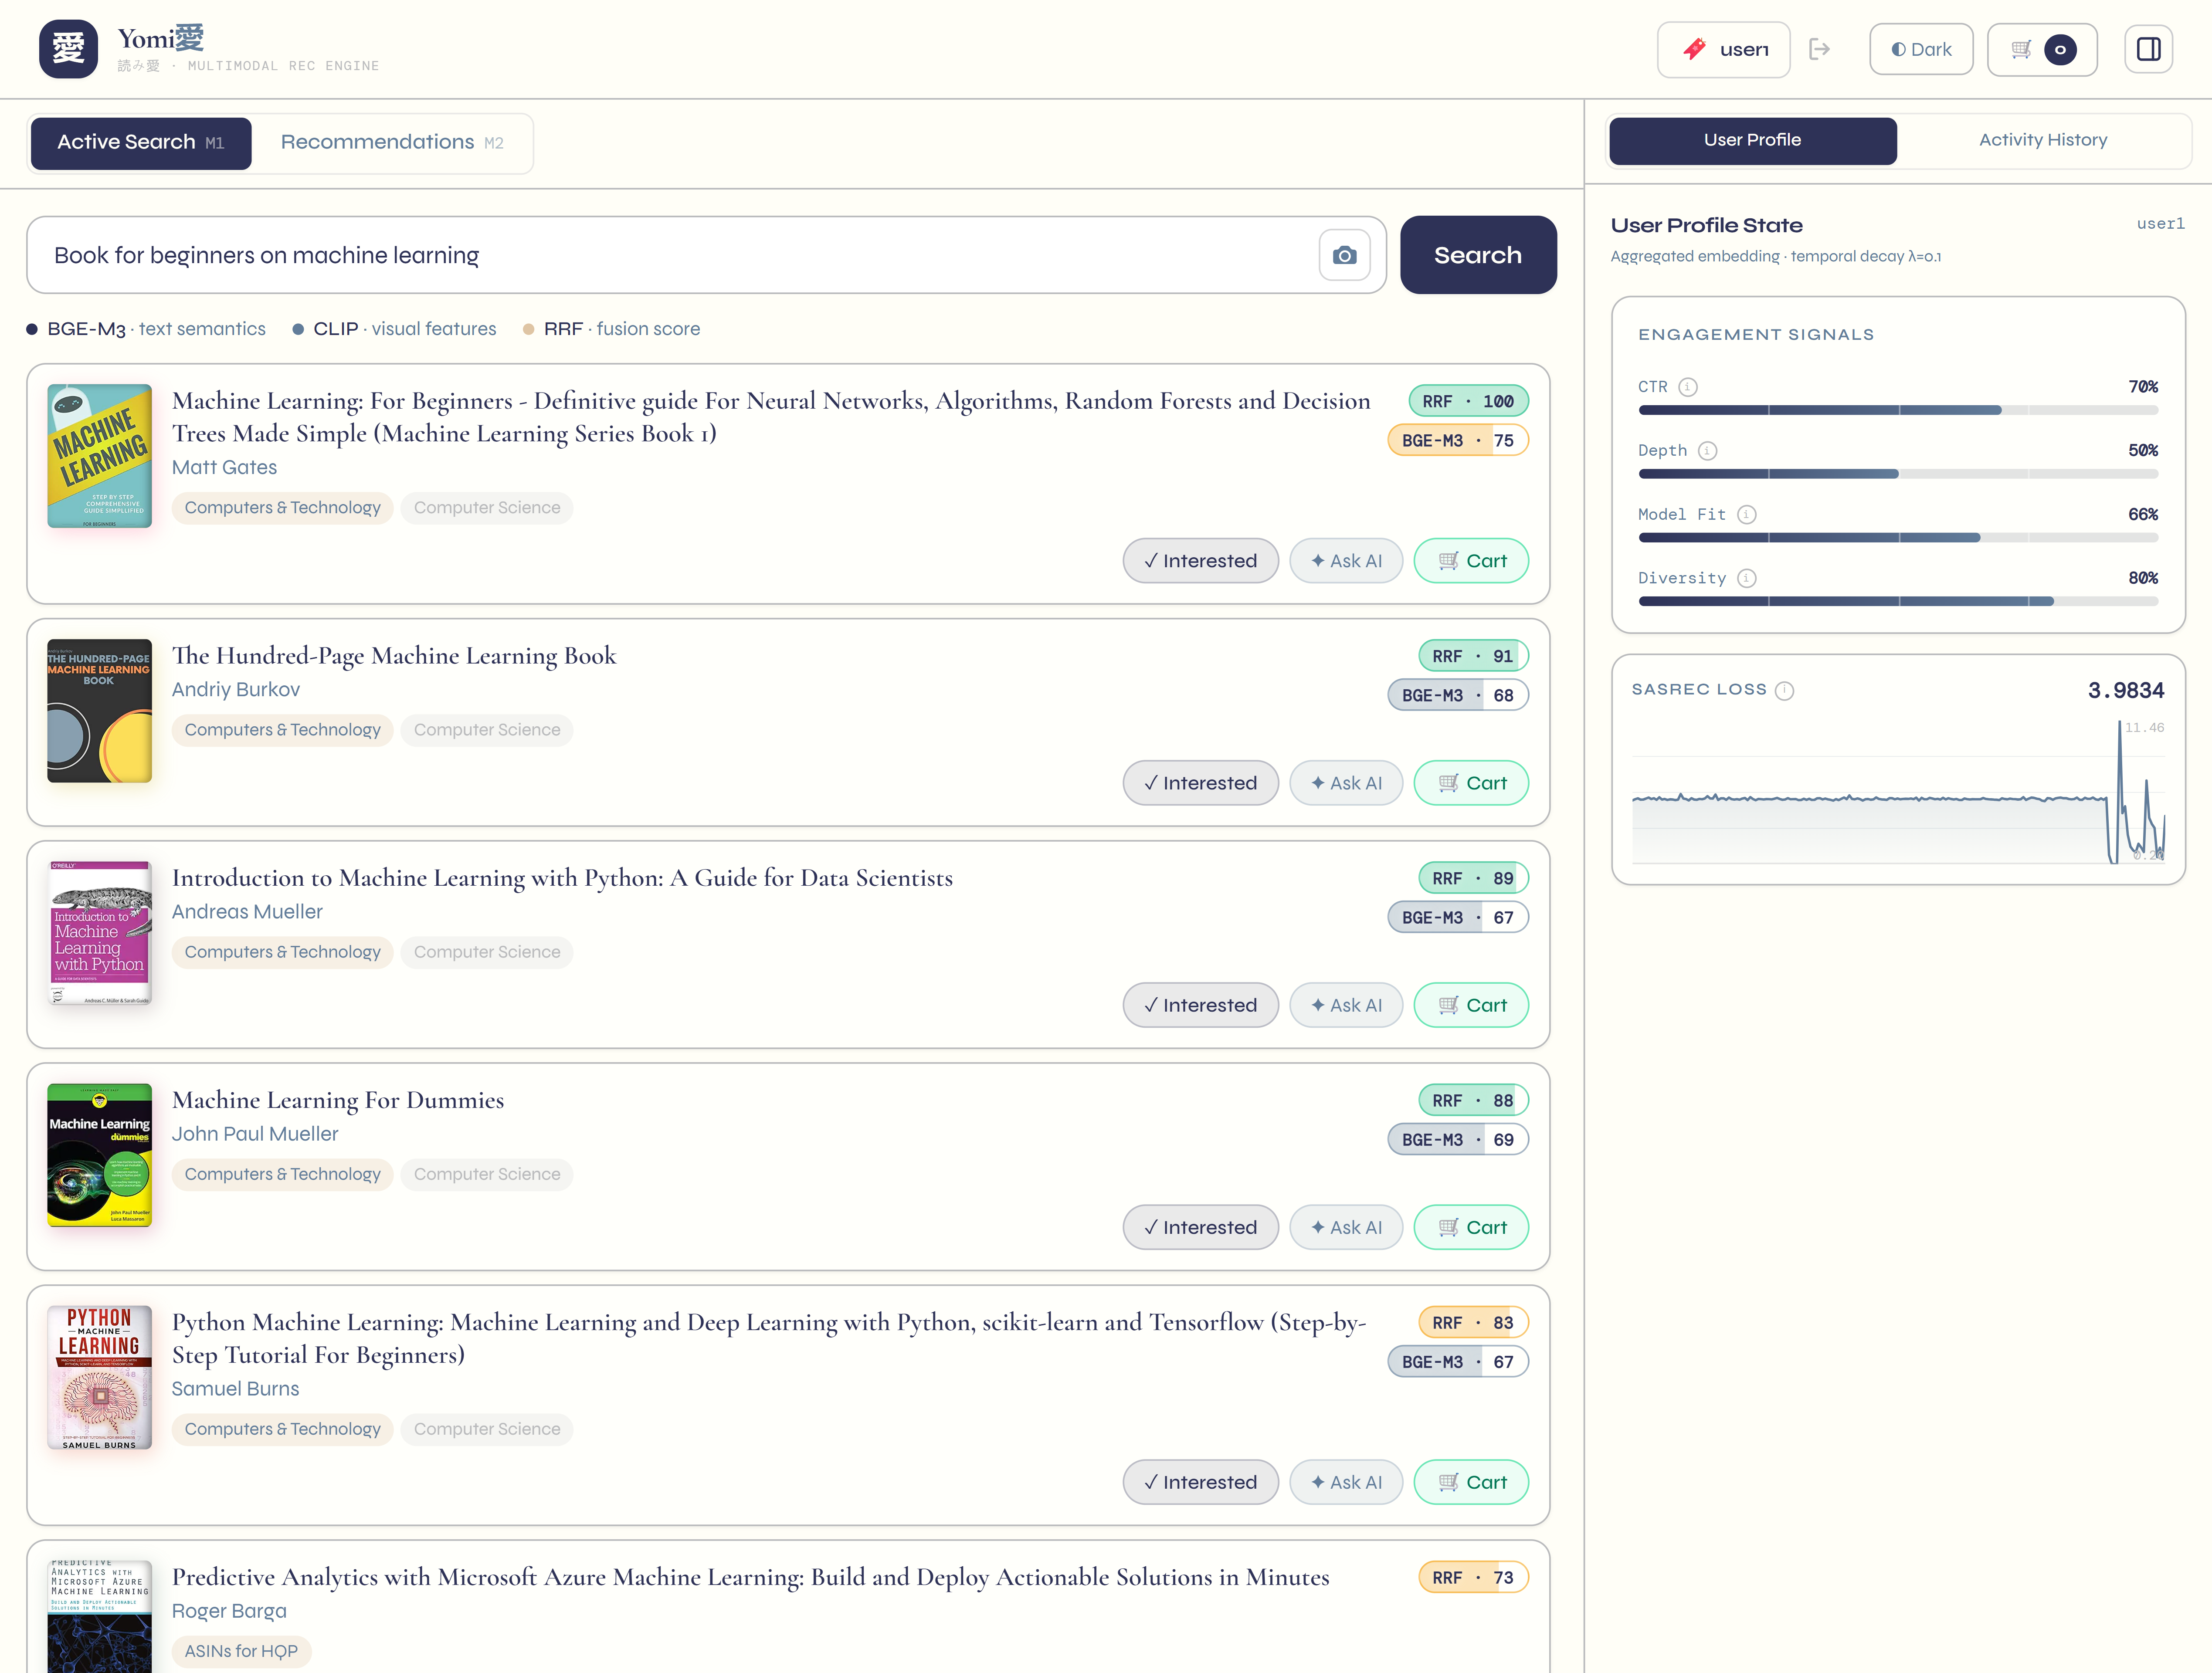
\includegraphics[width=0.80\textwidth]{images/chapter6/fig_search_text}
    \caption{Text query: RRF and BGE-M3 badges.}
    \label{fig:search_text}
\end{subfigure}

\vspace{8pt}

\begin{subfigure}{\textwidth}
    \centering
    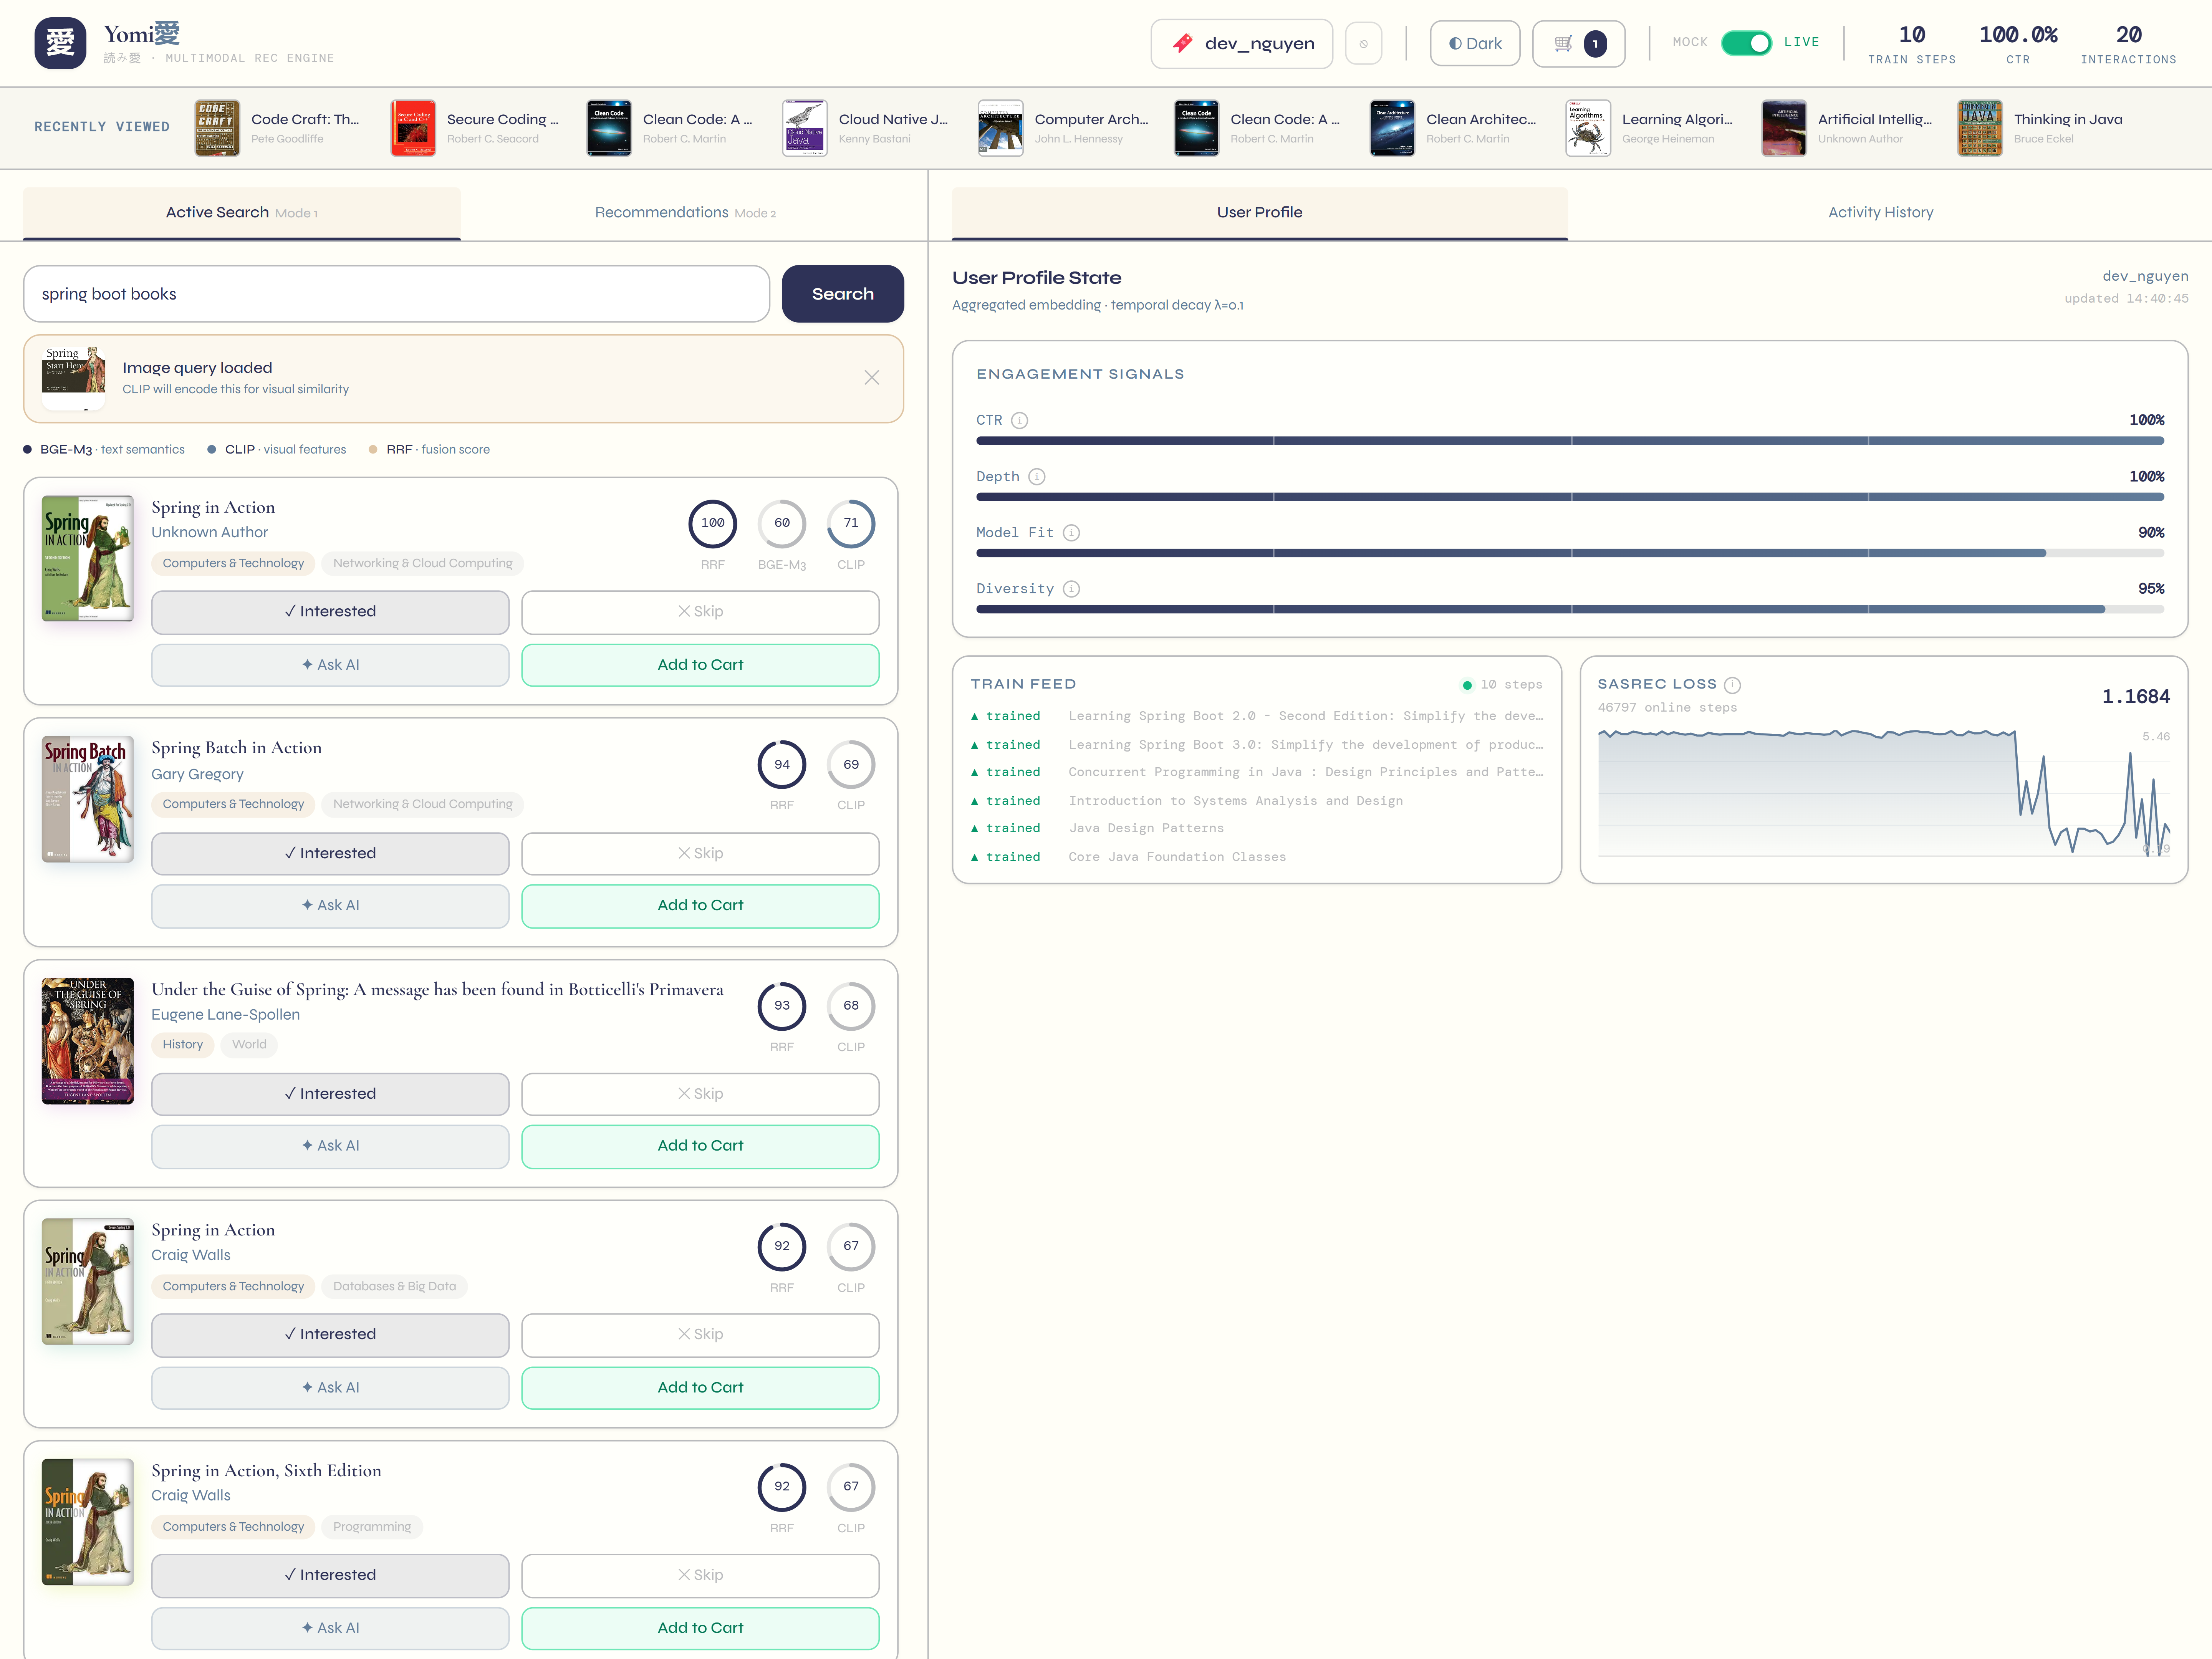
\includegraphics[width=0.80\textwidth]{images/chapter6/fig_search_multimodal}
    \caption{Combined text + image query: RRF, BGE-M3, and CLIP badges.}
    \label{fig:search_multimodal}
\end{subfigure}

\caption{Active Search results (Mode 1). Each result card presents cover image, title, author, genre, score badges, and four interaction controls: \textit{Interested}, \textit{Skip}, \textit{Ask AI} (streaming LLM popover), and \textit{Add to Cart}. (a)~Text-only query shows RRF and BGE-M3 badges. (b)~Combined text and image query additionally shows a CLIP badge, demonstrating the multimodal fusion path.}
\label{fig:search_demo}
\end{figure}

Each result card provides three interaction controls.
Interested logs a click event (reward 1.0), updates the in-memory user profile, and triggers a DIF-SASRec gradient step.
Add to Cart logs a cart event (reward 5.0), appends the item to the in-session cart, and triggers a gradient step.
Ask AI opens an inline streaming popover that calls \texttt{POST /ask\_llm\_stream}; the Qwen2.5 response is rendered progressively under Genre, Plot Summary, and Pitch headings as tokens arrive.

For image queries, the user clicks the camera icon button embedded within the search input to open an upload popover.
A drag-and-drop zone inside the popover accepts cover images; once an image is selected, a thumbnail preview confirms that the CLIP encoder will process it, and the popover can be dismissed.
If both text and image are supplied simultaneously, both encoders run in parallel and their candidate lists are fused by RRF before metadata hydration.

\subsection{Personalised Recommendation Flow}

After a user accumulates at least five interactions, the Recommendations tab (Mode 2) switches from cold-start to personalised mode.
A toast notification confirms the transition to personalised mode.

Figure~\ref{fig:rec_demo} shows the recommendation panel for a warm user.

\begin{figure}[htbp]
\centering
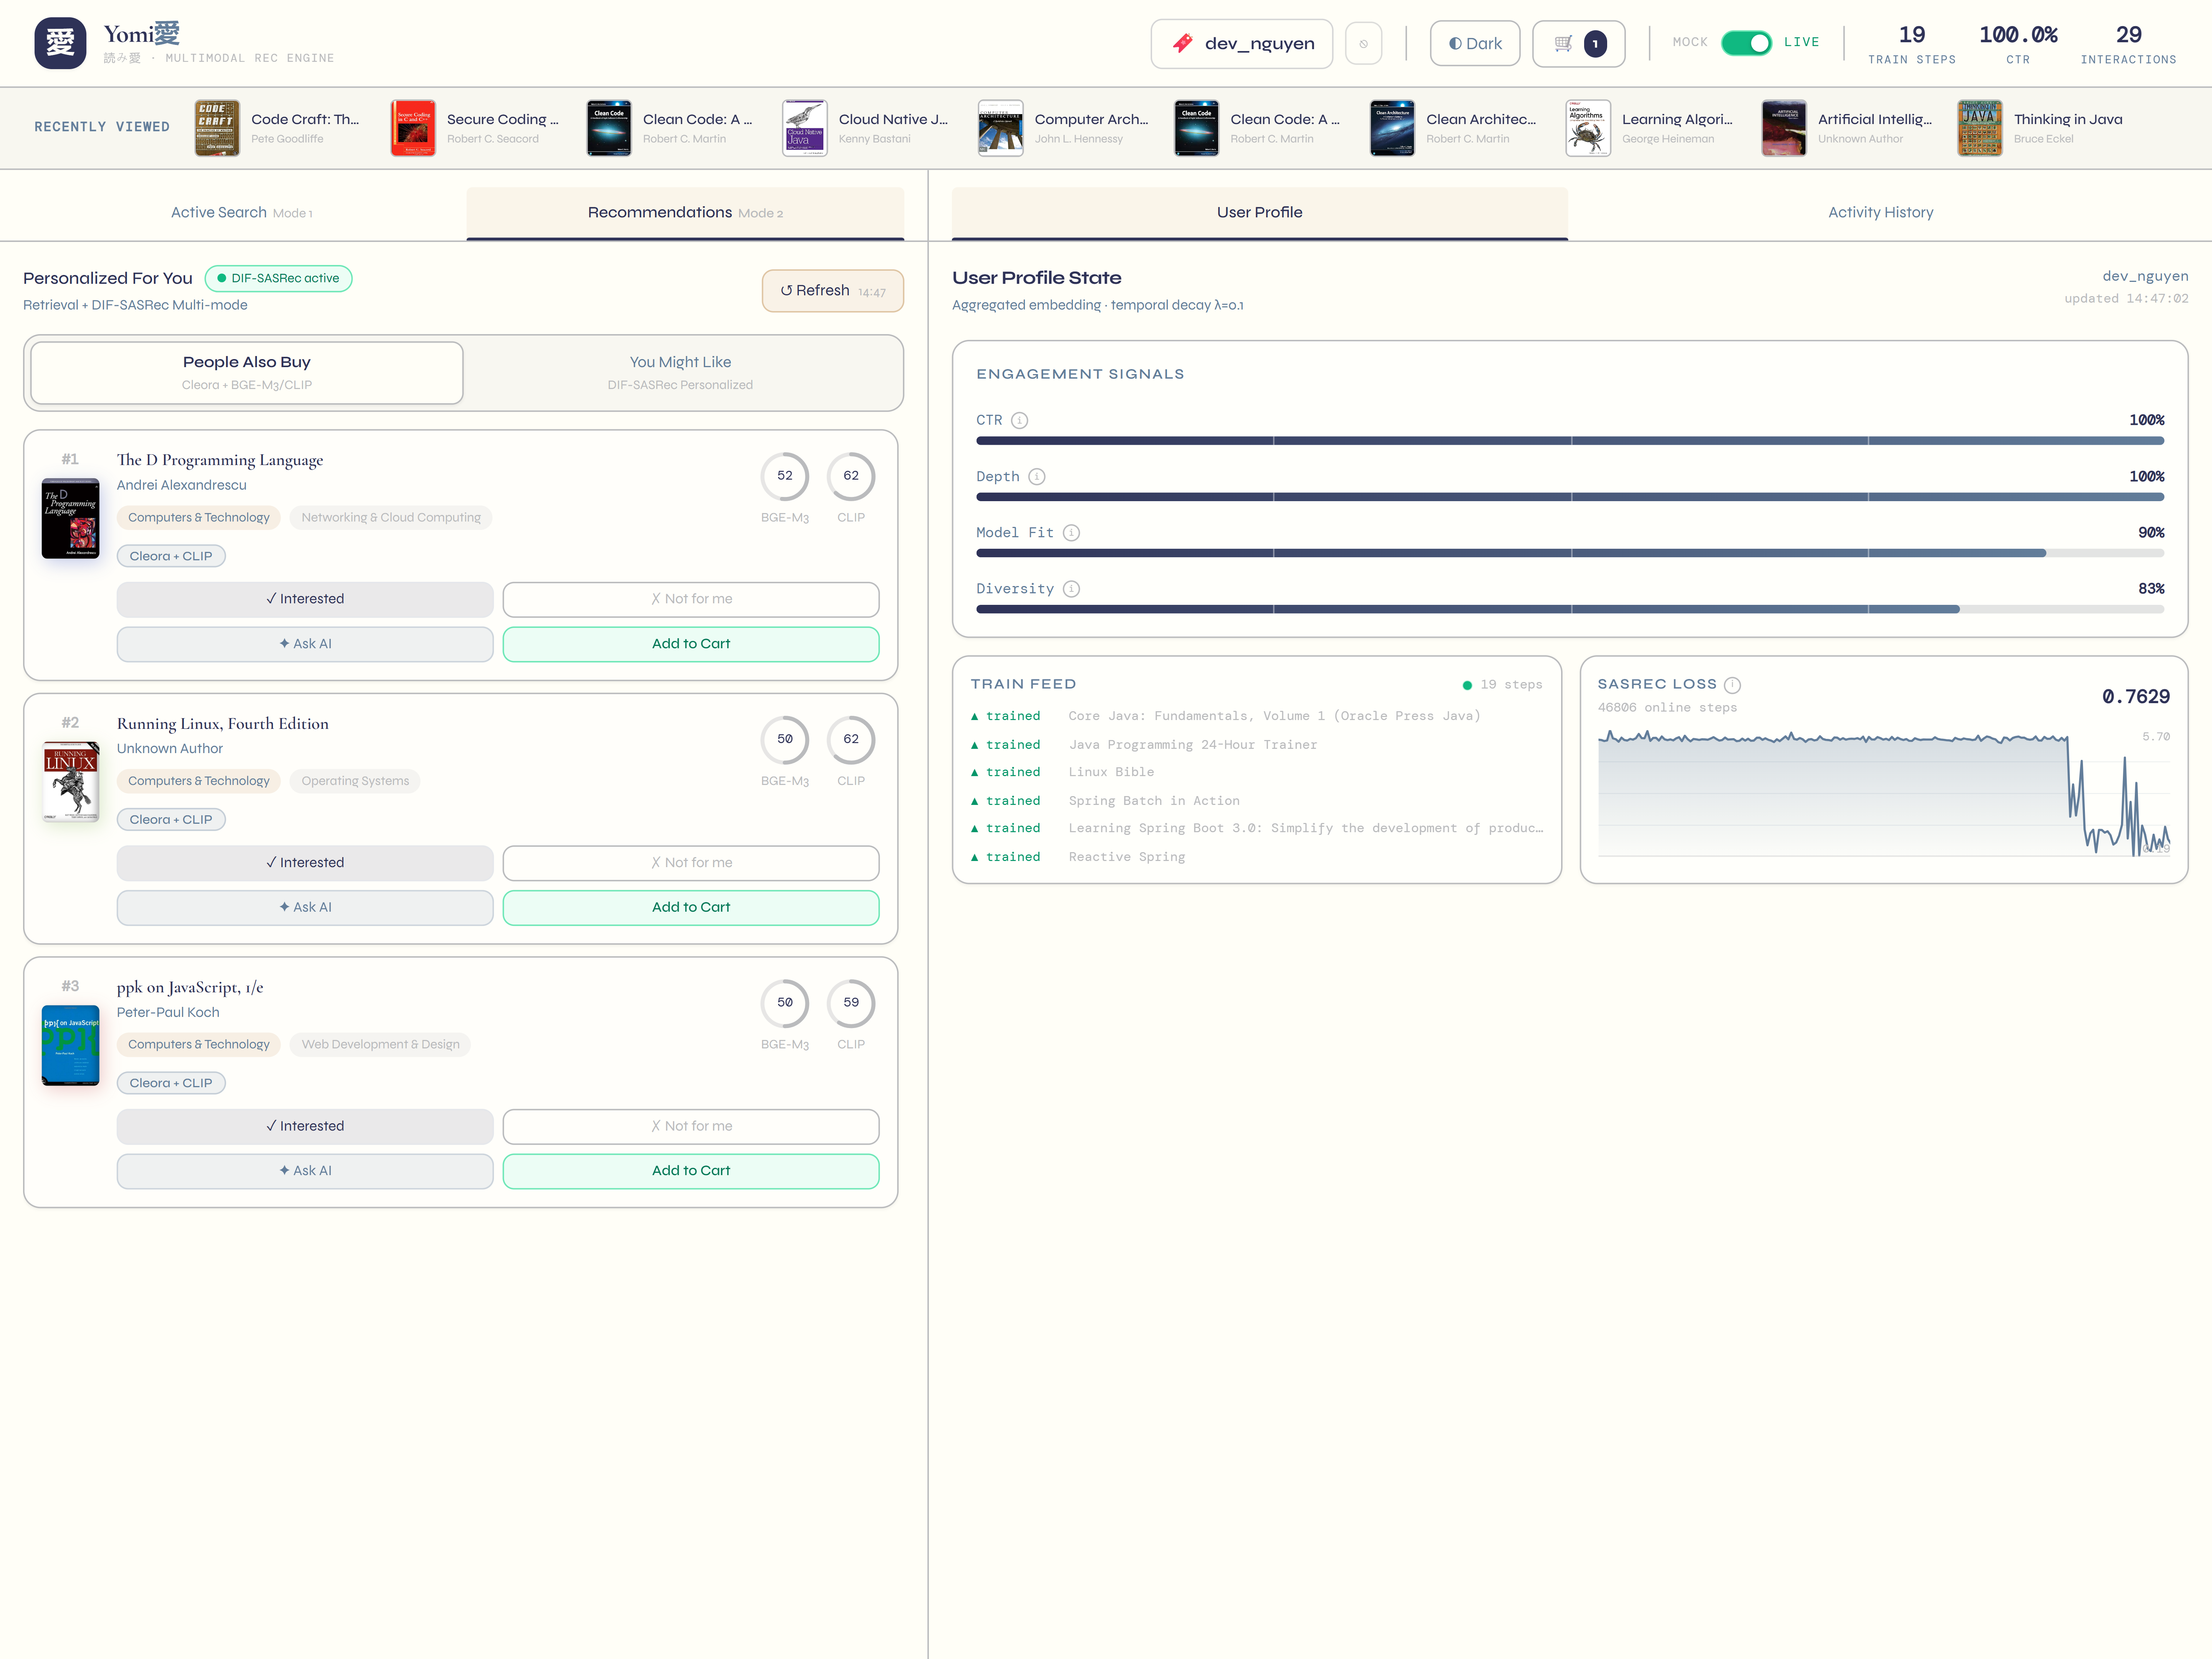
\includegraphics[width=0.92\textwidth]{images/chapter6/fig_rec_pab}
\caption{Personalised Recommendations (Mode 2) for a warm user, displayed as two side-by-side columns.
The People Also Buy column (Pipeline~A) surfaces Cleora co-purchase neighbours re-ranked by the user's BGE-M3 or CLIP profile vector, with cosine-similarity score badges and a \textit{Cleora~+~BGE-M3} or \textit{Cleora~+~CLIP} layer tag on each card.
The You Might Like column (Pipeline~B) applies the DIF-SASRec sequential model, with a SASRec score badge and a \textit{DIF-SASRec} layer tag.
The input-sequence strip above both columns displays the user's most recent click and cart interactions in chronological order, making the model's input visible.}
\label{fig:rec_demo}
\end{figure}

The input-sequence strip is displayed above both recommendation columns when personalised mode is active.
This strip shows the user's most recent click and cart interactions — up to eight items — in chronological order, representing the exact sequence that DIF-SASRec reads when generating the next-item prediction.
The strip makes the sequential model's input visible to the user, providing an explanation for why specific items were recommended.

Recommendations are refreshed automatically every three new interactions.
A manual refresh button forces an immediate reload and displays the last-updated timestamp beside its label.
Items that are new since the previous refresh are highlighted for four seconds.

\subsection{Online Learning Observation}

Every click or cart event triggers a sampled softmax gradient step on the user's personal DIF-SASRec checkpoint.
The SASRec Loss sparkline in the right-side profile panel shows the full loss history as a filled area chart.
A dashed divider marks the boundary between the pretraining phase (checkpoint-loaded, high loss scale) and the online fine-tuning phase (per-user gradient steps, lower scale).
An information tooltip beside the chart title explains the expected scale difference, noting that pretraining uses 512 hard negatives whereas online training samples from the full 3-million-item catalogue, producing a structurally lower loss.
When a gradient step fires, a transient loss-decrease badge is displayed beside the current loss value for 2.5 seconds, confirming that the model has updated.

\section{Search and Retrieval}
\label{sec:app_retrieval}

\subsection{API Contract}

Search is exposed via a single endpoint, \texttt{POST /search}, which accepts a JSON body with three optional fields:

\begin{itemize}
    \item \texttt{query} (string, default \texttt{""}): the text query, in any of the 19 supported languages.
    \item \texttt{image\_base64} (string, optional): a base64-encoded image for CLIP visual search.
    \item \texttt{top\_k} (integer, default 20): number of results to return.
\end{itemize}

The response is a JSON object containing a \texttt{results} array of hydrated item records (ASIN, title, author, genre, description, cover URL, relevance score, and per-modality similarity scores when applicable), a \texttt{total} count, a \texttt{live\_encoding} flag, and the echoed \texttt{query} string.
An optional \texttt{debug=true} query parameter appends a \texttt{\_debug\_timings} dictionary to the response, reporting per-stage latency in milliseconds (translation, text encoding, CLIP encoding, FAISS search, BM25 re-ranking, metadata hydration, and total).

\subsection{Retrieval Pipeline}

The internal pipeline executed by the \texttt{POST /search} handler is:

\begin{enumerate}
    \item \textbf{Language detection and translation}: the \texttt{lingua} detector identifies the input language in under 1\,ms. Non-English queries are translated to English by the NLLB-200 pipeline (Section~\ref{sec:nllb_pipeline}).
    \item \textbf{Parallel encoding}: text and image are encoded concurrently via an \texttt{anyio} task group. Each encoder runs in a background thread to avoid blocking the async event loop.
    \item \textbf{FAISS HNSW search}: the text vector is queried against \nolinkurl{bge_index_hnsw.faiss}; the image vector (if present) is queried against the CLIP HNSW index. Both retrieve 100 candidates.
    \item \textbf{Tantivy BM25 re-ranking}: the original query string is searched against the Tantivy full-text index to retrieve a ranked keyword hit list.
    \item \textbf{RRF fusion}: the HNSW and BM25 candidate lists are fused by Reciprocal Rank Fusion~\cite{cormack2009rrf} to produce a single ranked list.
    \item \textbf{Metadata hydration}: each ASIN in the final list is resolved against the in-memory DataFrame to attach display metadata.
\end{enumerate}

\subsection{Profile-Based Retrieval}

The \texttt{GET /recommend} endpoint uses a separate retrieval path.
For authenticated warm users, the profile manager fetches the user's most recent click sequence and computes a mean-pool BGE-M3 profile vector.
Pipeline~A queries the Cleora FAISS index (\texttt{IndexFlatIP}) with this profile vector, returning the 50 nearest co-purchase neighbours.
Pipeline~B retrieves item embeddings for the candidate set from the flat BGE-M3 index using the \texttt{reconstruct(i)} operation (HNSW indices do not support reconstruction, which is why the flat index is maintained separately), and applies the content veto filter before returning the DIF-SASRec top items.

\section{Additional Application Features}
\label{sec:app_other}

\subsection{User Authentication}

Authentication is handled by a full-screen login gate rendered before the main application.
The flow proceeds in three stages: the user enters a user ID and submits; the frontend calls \texttt{POST /auth/check}; if the ID is found in MongoDB the session begins immediately, and if not, a confirmation prompt offers account creation via \texttt{POST /auth/create} or the option to re-enter a different ID.
A Continue as Guest button on the login page generates a random \texttt{guest\_XXXXXX} identifier and bypasses both checks.
No password is stored or required at any point.
The resolved user ID is persisted in \texttt{localStorage}; subsequent visits load it and bypass the gate automatically.

\subsection{Not Interested}

Each book card provides a Not Interested button.
Clicking it immediately removes the item from the current recommendation panels on the frontend and sends a \texttt{POST /interact} request with \texttt{action = "not\_interested"}.
The backend stores the item identifier in a per-user Redis set (\texttt{user:\{id\}:blocked}); subsequent calls to \texttt{GET /recommend} filter out any blocked items before enriching the candidate lists, so the dismissed book will not reappear across sessions.
No gradient step is triggered for not-interested events.

\subsection{Interaction Logging and Online Training}

The \texttt{POST /interact} endpoint accepts \texttt{user\_id}, \texttt{item\_id}, and \texttt{action} (\texttt{click} or \texttt{not\_interested}).
For click actions, the endpoint borrows a DIF-SASRec agent from the pool, loads the user's personal checkpoint, runs one sampled softmax gradient step, saves the updated checkpoint, and returns the resulting \texttt{sasrec\_loss} value.
Not-interested actions are written to a per-user Redis blocked set with no training step.
The frontend appends the returned loss value to the sparkline on response, providing sub-second visual confirmation that the model has updated.

\subsection{Streaming LLM Book Assistant}
\label{sec:llm_assistant}

Each book card exposes an Ask AI button that opens an inline popover and calls \texttt{POST /ask\_llm\_stream}.
The Qwen2.5-1.5B-Instruct model~\cite{qwen2025} generates a structured response in three sections — Genre, Plot Summary, and Pitch — grounded by a retrieved external description that is semantically re-ranked by BGE-M3 before being passed to the model.
The response streams token-by-token into the popover via \texttt{TextIteratorStreamer}; the first token dismisses the loading indicator and content builds progressively.

\subsubsection{Grounding Pipeline}

To reduce hallucination and produce content-specific descriptions rather than generic summaries from training knowledge, the assistant uses a two-stage grounding pipeline before LLM generation:

\begin{enumerate}
    \item Context retrieval: The system first queries the Google Books API using \texttt{intitle:} and \texttt{inauthor:} operators for precision, falling back to a Wikipedia search with progressively broader queries (volume-specific → series-level → title-only) if Google Books returns no description.
    Rate-limiting logic backs off for 120 seconds after a 429 response, and an \texttt{@lru\_cache(maxsize=128)} stores results so repeated queries for the same title cost 0~ms.
    \item Semantic re-ranking: The raw retrieved text is split into sentences and each sentence is scored by cosine similarity to a query embedding \texttt{``plot summary arc story characters events \{title\} volume \{vol\}''}.
    The top-5 highest-scoring sentences are selected and concatenated as the grounding context.
    This step, implemented using the same BGE-M3 encoder used throughout the system, suppresses author biography sentences and publisher marketing text in favour of plot-relevant content.
\end{enumerate}

\subsubsection{Prompt Design}

The Qwen2.5 model is invoked with a two-turn chat template.
The system prompt constrains the model to rewrite only the provided context without drawing on its own training knowledge:

\begin{quote}
\texttt{You are a book description assistant. Your ONLY job is to rewrite the provided book description into the output format. Do NOT use your own knowledge. Do NOT add plot points not in the description. Use ONLY what is written in the description below.}
\end{quote}

The user turn specifies the exact output format and mirrors the Genre field from the item's metadata, preventing the model from inferring or inventing genre labels:

\begin{quote}
\texttt{Rewrite the description above into this exact format:}\\
\texttt{**Genre:** \{genre\}}\\
\texttt{**Plot Summary:** [2--3 sentences using ONLY the description above]}\\
\texttt{**Pitch:** [1 sentence on why to read this specific volume]}\\
\texttt{Do not add anything not in the description.}
\end{quote}

Generation uses greedy decoding (\texttt{do\_sample=False}) with a 200-token budget.
Greedy decoding is preferred over sampling because the structured output format requires exact heading placement; temperature-sampled outputs occasionally reorder or omit headings.
If no grounding context is available (e.g., the item has no Google Books or Wikipedia entry), a static fallback response is emitted without invoking the model, avoiding a generation that would be entirely hallucinated.

\subsection{User Profile Endpoint}

\texttt{GET /profile?user\_id=\{id\}} returns aggregated engagement statistics: total interaction count, total search count, click-through rate, and a hydrated list of the ten most recent interactions with full item metadata.
The frontend uses this response to populate the \texttt{ProfileRadar} chart and the Activity History tab.

\subsection{Health Check}

\texttt{GET /health} reports the readiness status of each loaded component, including FAISS indices, encoders, and the AgentPool.
It is intended for infrastructure monitoring and can be queried by external health-check probes to determine when the server is ready to serve traffic.

\section{System Performance Characteristics}
\label{sec:app_performance}

\subsection{Endpoint Latency}

Table~\ref{tab:endpoint_latency} reports warm-cache latency for each primary API endpoint measured under single-user sequential load on the development machine (NVIDIA GPU, 16~GB VRAM, 32~GB RAM).
``Warm cache'' means the FAISS indices are memory-mapped and paged in, the NLLB model is warmed up, and the target user's DIF-SASRec checkpoint has been loaded at least once (OS page cache warm).

\begin{table}[H]
\centering
\caption{Warm-cache endpoint latency (single-user sequential load).}
\label{tab:endpoint_latency}
\begin{tabular}{p{4.2cm} c c c p{4.6cm}}
\hline
\textbf{Endpoint} & \textbf{P50} & \textbf{P95} & \textbf{P99} & \textbf{Bottleneck} \\
\hline
\texttt{POST /search} (EN query)      & 59\,ms   & 85\,ms   & 110\,ms  & BGE-M3 encode + HNSW \\
\texttt{POST /search} (VI query)      & 61\,ms   & 92\,ms   & 118\,ms  & NLLB translate + encode \\
\texttt{POST /search} (text + image)  & 63\,ms   & 98\,ms   & 127\,ms  & Parallel CLIP + BGE-M3 \\
\texttt{GET /recommend} (warm user)   & 95\,ms   & 140\,ms  & 210\,ms  & DIF-SASRec checkpoint load \\
\texttt{POST /interact} (click)        & 320\,ms  & 480\,ms  & 620\,ms  & Checkpoint save to disk \\
\texttt{POST /interact} (not\_interested) & 4\,ms & 8\,ms    & 12\,ms   & Redis SADD only \\
\texttt{GET /profile}                 & 12\,ms   & 22\,ms   & 35\,ms   & MongoDB query + hydration \\
\texttt{POST /ask\_llm\_stream}       & 3{,}200\,ms & 5{,}100\,ms & — & Qwen2.5 generation (200 tokens) \\
\hline
\end{tabular}
\end{table}

Search latency is well within the 100\,ms interactive threshold for all query types.
The \texttt{POST /interact} endpoint for click events is noticeably slower (P50 320\,ms) because it includes a DIF-SASRec gradient step and checkpoint serialisation; not-interested events bypass the gradient step entirely (a single Redis \texttt{SADD}) and return in under 5\,ms.
The streaming LLM assistant has the highest absolute latency (P50 3.2 seconds for a full 200-token response), but because it streams token-by-token the user sees the first output token within approximately 200--400\,ms of the request, making the perceived responsiveness acceptable.

\subsection{Memory Footprint}

Table~\ref{tab:memory_footprint} summarises the in-memory footprint of all loaded components at steady state.

\begin{table}[H]
\centering
\caption{System memory footprint at steady state.}
\label{tab:memory_footprint}
\begin{tabular}{p{5.0cm} r r p{4.8cm}}
\hline
\textbf{Component} & \textbf{RAM} & \textbf{VRAM} & \textbf{Notes} \\
\hline
BGE-M3 text encoder          & —           & 560\,MB      & fp16, loaded once \\
CLIP image encoder            & —           & 340\,MB      & fp16, lazy-loaded \\
NLLB-200 translation model    & —           & 480\,MB      & int8 quantised, lazy-loaded \\
AgentPool (8\,$\times$\,DIF-SASRec) & —   & 1{,}184\,MB  & 148\,MB/agent (weights + AdamW) \\
Qwen2.5-1.5B-Instruct        & —           & 1{,}800\,MB  & fp16, lazy-loaded \\
FAISS HNSW (BGE-M3)          & 1{,}900\,MB & —            & Memory-mapped \\
FAISS Flat (BGE-M3)          & 3{,}200\,MB & —            & Memory-mapped \\
FAISS HNSW (CLIP)            & 680\,MB     & —            & Memory-mapped \\
Cleora NPZ + FAISS L2         & 310\,MB     & —            & CPU; hot-swappable \\
Tantivy BM25 index            & 820\,MB     & —            & Read-only, OS cache \\
\texttt{item\_metadata} DataFrame & 1{,}100\,MB & —        & In-memory Parquet \\
MongoDB + Redis (Docker)      & 480\,MB     & —            & Shared container memory \\
\hline
\textbf{Total (all warm)}    & $\approx$8.5\,GB & $\approx$4.4\,GB & \\
\hline
\end{tabular}
\end{table}

The largest single VRAM consumer is the AgentPool at 1.18~GB, followed by Qwen2.5 at 1.8~GB.
Not all components are loaded simultaneously: CLIP and NLLB are lazy-loaded on first use, and Qwen2.5 is loaded only if the LLM assistant is invoked.
A deployment without the LLM assistant reduces VRAM to approximately 2.6~GB, which fits within a consumer GPU with 8~GB VRAM.
The FAISS flat index (3.2~GB RAM) is the largest RAM consumer; in a memory-constrained environment it can be replaced by the HNSW index for production-only deployments at the cost of exact-reconstruction capability.

\subsection{Startup Sequence}

The server completes its startup sequence in three phases:
\begin{enumerate}
    \item Critical path (blocking, $\approx$8\,s): FAISS indices are memory-mapped, the Cleora NPZ is loaded, item metadata is read from Parquet, and the Tantivy index is opened. The \texttt{/health} endpoint returns \texttt{ready: false} until this phase completes.
    \item ML model loading ($\approx$12\,s): BGE-M3 and the AgentPool (8 agents × DIF-SASRec) are loaded sequentially on the GPU.
    \item Lazy warmup: NLLB and CLIP are warmed on first use; Qwen2.5 is loaded on the first \texttt{/ask\_llm\_stream} call. The \texttt{/health} endpoint returns \texttt{ready: true} after phase 2; the first cold Vietnamese query and the first LLM call each incur a one-time warm-up cost of 3--5\,s.
\end{enumerate}
Total time from process start to \texttt{ready: true} is approximately 20 seconds, dominated by GPU memory allocation for the eight AgentPool instances.


\chapter{Conclusion}
\textit{This chapter summarizes the achievements of the Capstone Project, evaluates the objectives established by the team, and proposes future enhancements for the system.}
\section{Summary of Achievements}
\label{sec:conclusion_summary}

Chapter~2 reviewed the theoretical foundations underpinning the system: sequential recommendation via self-attention~\cite{kang2018self,sun2019bert4rec}, co-purchase graph embedding via Cleora~\cite{rychalska2021cleora}, approximate nearest-neighbour search via HNSW~\cite{malkov2018hnsw}, large-scale similarity indexing via FAISS~\cite{johnson2021faiss}, multilingual encoding via BGE-M3~\cite{chen2024bge}, and Reciprocal Rank Fusion for retrieval combination~\cite{cormack2009rrf}.
These methods were selected on the basis of empirical performance, latency characteristics, and compatibility with the existing data platform.

Chapter~3 analysed the limitations of the prior system.
The legacy GRU-SeqDQN recommendation module achieved HR@10 = 0.1031 — statistically indistinguishable from the random baseline of 0.1000 — due to the fixed-size GRU bottleneck and the intractable 3-million-item DQN action space.
The BLaIR text encoder produced Precision@10 $\leq 0.05$ on Vietnamese queries, making the system functionally unusable for the target multilingual user base.
The FAISS flat index incurred a P50 search latency of 612.19\,ms and a 45-second startup loading penalty, precluding interactive use.

Chapter~4 introduced four infrastructure changes to address these shortcomings.
BLaIR was replaced by BGE-M3, and the GRU-SeqDQN module was replaced by a dual-mode architecture comprising Pipeline~A (Cleora + BGE-M3) and Pipeline~B (DIF-SASRec).
A three-stage NLLB-200 translation pipeline extended query support to 19 non-English languages.
Parallel text and CLIP encoding was achieved via an \texttt{anyio} task group.
The flat FAISS index was replaced by a dual HNSW/flat strategy loaded via memory mapping, and a three-stage incremental Cleora refit pipeline was introduced to incorporate new interactions without restarting the server.

Chapter~5 evaluated these changes quantitatively.
Pipeline~A (Cleora + BGE-M3) achieves HR@10 = 0.9047 and Pipeline~B (DIF-SASRec) achieves HR@10 = 0.7745 on 100{,}000 held-out test users, both substantially above the Content Baseline (0.4346) and the prior GRU-SeqDQN approach (0.1031).
The DIF-SASRec result is stable across five random evaluation seeds (standard deviation $\sigma = 0.0024$).
Multilingual search performance reached Precision@10 = 0.55 on long Vietnamese queries under BGE-M3, compared to 0.05 under BLaIR.
Warm-cache end-to-end search latency was reduced from 1{,}102\,ms to 59\,ms.

Chapter~6 presented the deployed book discovery application, demonstrating the end-to-end integration of all components: the login gate, the multimodal search interface (text, image, and fused), the dual-panel recommendation view with the DIF-SASRec input-sequence strip, the real-time profile panel with the training loss sparkline, and the streaming Qwen2.5 book assistant.

---

\section{Evaluation of Objectives}
\label{sec:conclusion_objectives}

Table~\ref{tab:objectives} evaluates each objective stated in Section~\ref{sec:goals} against the experimental evidence.

\begin{table}[H]
\centering
\caption{Evaluation of project objectives against experimental evidence.}
\label{tab:objectives}
\begin{tabular}{p{5.8cm} p{2.2cm} p{5.5cm}}
\hline
\textbf{Objective} & \textbf{Status} & \textbf{Evidence} \\
\hline
Design a dual-mode recommendation pipeline (Pipeline~A + Pipeline~B) &
Met &
Table~\ref{tab:main_results}: Pipeline~A HR@10 = 0.9047, Pipeline~B HR@10 = 0.7745 \\

Achieve substantial improvement over the prior GRU-SeqDQN baseline &
Met &
HR@10 increased from 0.1031 (GRU-SeqDQN) to 0.9047 (Pipeline~A) and 0.7745 (Pipeline~B), Table~\ref{tab:main_results} \\

Enable multilingual semantic search with $\geq 5\times$ Precision@10 improvement on Vietnamese queries &
Met &
Precision@10 on long Vietnamese queries: 0.0500 (BLaIR) $\to$ 0.5500 (BGE-M3), an 11$\times$ improvement (Table~\ref{tab:query_retrieval}) \\

Reduce warm-cache end-to-end search latency below 100\,ms &
Met &
Latency reduced from 1{,}102\,ms to 59\,ms (warm cache), Table~\ref{tab:latency_stages} \\

Deploy an interactive application integrating all platform components &
Met &
Chapter~6 presents the deployed book discovery application combining multimodal search, dual-pipeline recommendations, online DIF-SASRec fine-tuning, and the Qwen2.5 LLM assistant \\
\hline
\end{tabular}
\end{table}

All five objectives are met.
The clearest improvement is in recommendation quality: the prior GRU-SeqDQN approach scored HR@10 = 0.1031, near random, while Pipeline~A reaches 0.9047 and Pipeline~B reaches 0.7745 on the same test set.

---

\section{Research Contributions}
\label{sec:contributions}

This project makes the following specific technical contributions:

\begin{enumerate}
    \item \textbf{Incremental Cleora hot-swap pipeline.}
    A three-stage fault-isolated pipeline (delta export → graph augmentation → atomic in-memory swap) enables the Cleora co-purchase embeddings to be updated from live interaction logs without server restart.
    The atomic swap guarantees that concurrent in-flight recommendation requests observe a consistent index state throughout the update.

    \item \textbf{DIF-SASRec decoupled attention with learnable fusion scalar.}
    The implementation extends the original DIF-SASRec formulation with a sigmoid-gated fusion scalar $\alpha$ that is initialised to favour the category stream ($\alpha_0 = 0.7$) and is learned jointly during pretraining.
    This allows the model to adapt the relative importance of content and category attention to the characteristics of the Amazon Books domain.

    \item \textbf{Min-max normalised DIF-SASRec intent scores for UI transparency.}
    Raw DIF-SASRec dot-product scores are unbounded and vary by orders of magnitude across users.
    The backend applies per-request min-max normalisation so that the top-ranked candidate always receives score 1.0 and all remaining candidates are proportional to their dot-product gap.
    This makes the per-card score badges on the \textit{You Might Like} panel directly interpretable by users.

    \item \textbf{Dual-panel recommendation interface with per-pipeline attribution.}
    The frontend exposes two recommendation panels that directly mirror the two backend pipelines, with per-card layer tags (\textit{Cleora\,+\,BGE-M3}, \textit{Cleora\,+\,CLIP}, \textit{DIF-SASRec}) and the DIF-SASRec input-sequence strip.
    This design makes the recommendation provenance visible to users and provides a basis for future A/B testing of pipeline variants.

    \item \textbf{training loss sparkline as training transparency.}
    A live SVG sparkline in the right-panel profile view plots the full per-user training loss history with an annotated phase boundary between pretraining and online fine-tuning.
    This provides immediate, per-interaction visual confirmation that the DIF-SASRec model has updated — a transparency mechanism with no equivalent in existing open-source recommendation systems.

    \item \textbf{BGE-M3-based semantic re-ranking for LLM grounding.}
    Rather than passing raw Wikipedia or Google Books extracts to the Qwen2.5 assistant, the grounding pipeline uses the same BGE-M3 encoder deployed throughout the system to select the top-5 plot-relevant sentences from the retrieved text.
    This suppresses author biography sentences and marketing language without requiring a separate re-ranking model.
\end{enumerate}

---

\section{Generalisation to Other Domains}
\label{sec:generalisation}

The system was designed with a modular architecture in which domain-specific and domain-agnostic components are cleanly separated.
Table~\ref{tab:generalisation} assesses the portability of each component to a hypothetical new domain.

\begin{table}[htbp]
\centering
\caption{Component portability to a new recommendation domain.}
\label{tab:generalisation}
\begin{tabular}{p{4.0cm} p{2.0cm} p{6.5cm}}
\hline
\textbf{Component} & \textbf{Portability} & \textbf{Notes} \\
\hline
FastAPI + React SPA framework & Drop-in & No domain coupling; only API schemas change \\
HNSW + FAISS retrieval        & Drop-in & Accepts any fixed-dimensional embedding \\
RRF fusion                    & Drop-in & Parameter-free; works with any pair of ranked lists \\
NLLB translation pipeline     & Drop-in & Supports 202 languages regardless of domain \\
Tantivy BM25 index            & Drop-in & Domain-agnostic text index \\
Interaction logging (Redis + MongoDB) & Drop-in & Schema generalises to any item-action event \\
BGE-M3 encoder                & Reusable & Multilingual; re-embedding required for new item catalogue \\
CLIP image index               & Reusable & Re-embedding required if image modality differs \\
AgentPool + checkpoint system  & Reusable & Architecture is independent of domain; pretraining required \\
DIF-SASRec pretrained weights  & Domain-specific & Pretrained on Amazon Books; retraining needed for new domain \\
Cleora co-purchase graph       & Domain-specific & Requires domain interaction logs to build the co-purchase graph \\
item\_metadata Parquet store   & Domain-specific & Schema (title, genre, image URL) maps naturally to many product domains \\
\hline
\end{tabular}
\end{table}

The retrieval infrastructure (HNSW, RRF, NLLB, Tantivy, Redis, MongoDB) requires no changes to support a new domain.
The encoder and model layers (BGE-M3, CLIP, DIF-SASRec) require re-embedding and retraining on domain-specific data, but the training code and serving infrastructure are reusable.
Only the Cleora graph is tightly coupled to the co-purchase interaction pattern; an analogous collaborative signal (e.g., co-view, co-play, co-purchase in another product domain) would enable direct reuse.

---

\section{Limitations}
\label{sec:conclusion_limitations}

Several limitations of the proposed system are identified.

\begin{itemize}
    \item \textbf{Incomplete catalogue coverage in Pipeline~A.}
    The Cleora co-purchase graph covers 375{,}280 items — 12.5\% of the full 3-million-item catalogue.
    Items outside the graph cannot be retrieved by Pipeline~A, contributing to the 2.6\% of test users (2{,}641) that neither pipeline serves (Section~\ref{sec:qualitative}).

    \item \textbf{Content veto over-filtering.}
    The cosine similarity threshold $\tau = 0.3$ in Pipeline~B occasionally filters out semantically legitimate candidates whose embeddings fall just below the threshold.
    This is particularly harmful for users with sparse histories, where the DIF-SASRec prediction may be the only available recommendation path.

    \item \textbf{HNSW recall degradation.}
    The HNSW index achieves a recall of 0.521 relative to exact flat search (Table~\ref{tab:hnsw_comparison}), meaning that 47.9\% of the nearest neighbours under the full index are not returned by the approximate index.
    The BM25 re-ranking stage partially compensates, but this gap may reduce recommendation quality for queries where exact top-$k$ proximity is critical.

    \item \textbf{Online fine-tuning latency on cold sessions.}
    The DIF-SASRec gradient step executes synchronously in the \texttt{POST /interact} request handler.
    For users with long interaction histories the checkpoint serialisation and deserialisation from disk introduces latency that grows proportionally with checkpoint size.

    \item \textbf{In-session cart state.}
    The shopping cart is held in React component state only and is not persisted to the backend.
    Cart contents are lost on page reload, preventing recovery of abandoned carts and limiting the cart signal from influencing Cleora graph updates across sessions.
\end{itemize}

---

\section{Future Work}
\label{sec:conclusion_future}

Several concrete directions for future improvement follow from the identified limitations.

\begin{itemize}
    \item \textbf{Expand the Cleora index to the full catalogue.}
    Extending the co-purchase graph from 375{,}280 to the full 3 million items would eliminate the catalogue boundary that causes Pipeline~A to fail for long-tail items.
    The incremental refit pipeline introduced in Section~\ref{sec:cleora_incremental} already supports partial augmentation; a batch re-embedding of the full catalogue with accumulated interaction data is the next step.

    \item \textbf{Adaptive content veto threshold.}
    Rather than a fixed threshold of $\tau = 0.3$, the veto could be relaxed to $\tau = 0.2$ or disabled entirely for users with fewer than 20 interactions, where over-filtering risk outweighs the benefit of semantic consistency enforcement.
    This directly addresses the sparse-user failure mode identified in Section~\ref{sec:qualitative}.

    \item \textbf{Asynchronous online fine-tuning.}
    Moving the DIF-SASRec gradient step from the synchronous \texttt{POST /interact} response path to a background task queue would decouple interaction logging latency from model update latency, allowing the training step to be batched and accelerated without impacting the user-facing response time.

    \item \textbf{Persistent cart and cross-session interaction signals.}
    Persisting cart events to MongoDB in the same manner as click and skip events would allow cart additions to contribute to Cleora graph updates across sessions, providing a higher-reward signal that currently disappears on page reload.

    \item \textbf{Extension to additional retrieval modalities.}
    The current retrieval pipeline combines text (BGE-M3) and visual (CLIP) signals.
    Incorporating structured metadata signals — genre taxonomy, publication year, reading-level classification — as additional FAISS or Tantivy filter axes would improve precision for queries that express constraints rather than pure semantic similarity (e.g., ``beginner-level machine learning books published after 2020'').
\end{itemize}

\input{sections/references}

\appendix
\chapter{API Endpoint Reference}
\label{app:api}

Table~\ref{tab:api_endpoints} documents the seven route groups exposed by the FastAPI backend, together with their HTTP method, path, and primary function.
All endpoints return JSON and are served at \texttt{http://localhost:8000} in the development configuration.

\begin{table}[H]
\centering
\caption{FastAPI backend endpoint reference.}
\label{tab:api_endpoints}
\begin{tabular}{p{1.6cm} p{5.0cm} p{6.4cm}}
\hline
\textbf{Method} & \textbf{Path} & \textbf{Function} \\
\hline
\multicolumn{3}{l}{\textit{Authentication}} \\
POST & \texttt{/auth/check}          & Check whether a user ID exists in MongoDB \\
POST & \texttt{/auth/create}         & Create a new user record and initialise an empty profile \\
\hline
\multicolumn{3}{l}{\textit{Search}} \\
POST & \texttt{/search}              & Multimodal query: accepts a text string and/or a base64-encoded image; returns top-$k$ items with RRF, BGE-M3, and CLIP score fields \\
\hline
\multicolumn{3}{l}{\textit{Recommendations}} \\
GET  & \texttt{/recommend}           & Dual-pipeline personalised recommendations; returns \texttt{people\_also\_buy} (Pipeline~A) and \texttt{you\_might\_like} (Pipeline~B) lists with per-item score and layer fields \\
\hline
\multicolumn{3}{l}{\textit{Interaction logging}} \\
POST & \texttt{/interact}            & Log a user interaction event (click, skip, or cart); triggers a DIF-SASRec Bellman-error gradient step for click and cart events; returns updated loss value \\
\hline
\multicolumn{3}{l}{\textit{User profile}} \\
GET  & \texttt{/profile}             & Return the user's in-memory profile: click sequence, recent interactions, BGE-M3 profile vector norm, session statistics (CTR, train steps, interactions), and Bellman-error loss history \\
\hline
\multicolumn{3}{l}{\textit{LLM assistant}} \\
POST & \texttt{/ask\_llm\_stream}    & Stream a Qwen2.5 book description response; returns an SSE stream of token chunks structured under \textbf{Genre}, \textbf{Plot Summary}, and \textbf{Pitch} headings \\
\hline
\multicolumn{3}{l}{\textit{Health check}} \\
GET  & \texttt{/health}              & Return service status, index loading state, and warm-up flag \\
\hline
\end{tabular}
\end{table}

\chapter{Extended Hyperparameter Tables}
\label{app:hyperparams}

Table~\ref{tab:app_model_config} extends the model configuration summary in Table~\ref{tab:model_config} with additional DIF-SASRec training details and FAISS index construction parameters.

\begin{table}[H]
\centering
\caption{Extended model and index hyperparameters.}
\label{tab:app_model_config}
\begin{tabular}{p{5.5cm} p{7.5cm}}
\hline
\textbf{Parameter} & \textbf{Value} \\
\hline
\multicolumn{2}{l}{\textit{DIF-SASRec — Architecture}} \\
Transformer blocks     & 4 \\
Attention heads        & 8 \\
Hidden dimension       & 512 \\
Feed-forward dimension & 2{,}048 \\
Dropout rate           & 0.1 \\
Max sequence length    & 200 \\
Total parameters       & $\approx$12.4M \\
\hline
\multicolumn{2}{l}{\textit{DIF-SASRec — Pre-training}} \\
Training users         & 100{,}000 \\
Epochs                 & 30 \\
Batch size             & 2{,}048 \\
Optimiser              & AdamW \\
Learning rate          & $10^{-4}$ with cosine annealing \\
Weight decay           & 0.01 \\
Hard negatives per step & 512 \\
\hline
\multicolumn{2}{l}{\textit{DIF-SASRec — Online fine-tuning}} \\
Trigger events         & click (reward 1.0), cart (reward 5.0) \\
Gradient steps per event & 1 \\
Online learning rate   & $10^{-5}$ \\
Negative sample pool   & full 3M-item catalogue \\
Checkpoint format      & per-user \texttt{.pt} file (disk) \\
\hline
\multicolumn{2}{l}{\textit{FAISS HNSW index (production)}} \\
Dimension              & 1{,}024 (BGE-M3) \\
Vectors                & 1{,}742{,}826 \\
HNSW $M$               & 32 \\
$\mathit{efConstruction}$ & 200 \\
Recall vs.\ flat index & 0.521 \\
P50 search latency     & 119.56 ms \\
\hline
\multicolumn{2}{l}{\textit{FAISS Flat index (evaluation)}} \\
Dimension              & 1{,}024 \\
Vectors                & 3{,}080{,}829 \\
P50 search latency     & 612.19 ms \\
\hline
\multicolumn{2}{l}{\textit{Cleora graph embedding}} \\
Graph type             & Co-purchase bipartite graph \\
Embedding dimension    & 1{,}024 \\
Items covered          & 375{,}280 \\
Refit threshold        & 50 new interactions \\
Refit stages           & delta export → augment → hot-swap \\
\hline
\multicolumn{2}{l}{\textit{RRF fusion}} \\
Constant $k$           & 60 \\
Candidates per source  & 100 (HNSW), 100 (BM25) \\
Output top-$k$         & 10 \\
\hline
\end{tabular}
\end{table}

\input{sections/appendixes/plan}
% add appendix later on

\end{document}
